% =====================================================================
%  Anatomía de un LLM — Fase 0 — Módulo 0.6
%  Cálculo integral y series
%  Compilar: latexmk -r ../latexmkrc P06-calculo-integral.tex
% =====================================================================
\documentclass[11pt,a4paper,twoside,openany]{book}
\usepackage{../estilo-apuntes}

\newcommand{\ApuntesCurso}{Anatomía de un LLM}
\newcommand{\ApuntesModulo}{Módulo 0.6}

% Notación propia del módulo
\newcommand{\N}{\mathbb{N}}
\newcommand{\Z}{\mathbb{Z}}
\newcommand{\Q}{\mathbb{Q}}
\newcommand{\dif}{\mathop{}\!d}
\newcommand{\Lsum}{\operatorname{L}}
\newcommand{\Usum}{\operatorname{U}}
\newcommand{\Rsum}{\operatorname{S}}
\newcommand{\eval}[3]{\bigl[#1\bigr]_{#2}^{#3}}

% Anclas de hiperenlace únicas para los enunciados (el contador se reinicia en cada tema)
\makeatletter
\@for\@env:={definicion,teorema,proposicion,lema,corolario,ejemplo,observacion}\do{%
  \expandafter\providecommand\csname theH\@env\endcsname{}%
  \expandafter\renewcommand\csname theH\@env\endcsname{\thechapter.\arabic{definicion}}}
\makeatother

\hypersetup{pdftitle={Módulo 0.6. Cálculo integral y series},pdfauthor={Anatomía de un LLM}}

\begin{document}
\frontmatter
% ------------------------------------------------------------------ Portada
\begin{titlepage}
\centering
\vspace*{2.5cm}
{\large\scshape Anatomía de un LLM}\par
\vspace{0.4cm}
{\normalsize Fundamentos matemáticos de los modelos de lenguaje}\par
\vspace{2.2cm}
\rule{\textwidth}{0.8pt}\par\vspace{0.5cm}
{\small\scshape Fase 0 \textperiodcentered\ Preliminares matemáticos}\par\vspace{0.3cm}
{\Huge\bfseries Módulo 0.6\par}\vspace{0.3cm}
{\LARGE Cálculo integral y series\par}
\vspace{0.5cm}\rule{\textwidth}{0.4pt}\par
\vspace{1.6cm}
{\large Apuntes del curso}\par
\vfill
{\small Edición de octubre de 2026}\par
\end{titlepage}

% ------------------------------------------------------- Presentación
\chapter*{Presentación del módulo}
\addcontentsline{toc}{chapter}{Presentación del módulo}
\markboth{Presentación del módulo}{}

El cálculo diferencial estudia cómo cambia una función; el cálculo integral estudia cómo se acumula. Los modelos de lenguaje usan las dos caras. Una probabilidad de una variable continua es la integral de una densidad, una esperanza es una integral ponderada y la constante que normaliza la distribución normal es la integral gaussiana. Las sumas infinitas aparecen al descontar recompensas futuras, al acumular medias exponenciales en los optimizadores y al aproximar funciones como $e^{x}$ o $\ln(1+x)$ por polinomios. Este módulo presenta la integral de Riemann, el teorema fundamental del cálculo y las técnicas de integración, extiende la integral a intervalos no acotados y estudia la convergencia de series numéricas y de series de potencias, con la misma organización que los cursos universitarios de cálculo de una variable y con una colección extensa de ejercicios resueltos paso a paso.

\section*{Objetivos}
Al finalizar el módulo, el estudiante debe ser capaz de:
\begin{enumerate}[label=\arabic*.]
  \item definir la integral de Riemann mediante sumas superiores e inferiores, calcular sumas de Riemann y demostrar las propiedades básicas de la integral;
  \item enunciar y demostrar el teorema del valor medio integral y las dos partes del teorema fundamental del cálculo, y usarlas para calcular integrales, derivar funciones definidas por integrales, hallar áreas y valores medios;
  \item calcular primitivas por sustitución, por partes, por fracciones simples y con identidades trigonométricas, y obtener fórmulas de reducción;
  \item decidir la convergencia de integrales impropias por cálculo directo o por comparación, y calcular la función Gamma en enteros y semienteros y la integral gaussiana;
  \item decidir la convergencia de series numéricas con los criterios de comparación, cociente, raíz, integral y de Leibniz, y acotar el error al truncarlas;
  \item hallar el radio de convergencia de una serie de potencias, obtener las series de Taylor de $e^{x}$, $\sin x$, $\cos x$, $\ln(1+x)$ y $(1+x)^{a}$ y demostrar que convergen a la función.
\end{enumerate}

\section*{Requisitos previos}
Matemáticas de bachillerato y los módulos 0.1 a~0.5 de esta fase: técnicas de demostración e inducción (0.1), sumatorios, la suma geométrica finita y la desigualdad de Bernoulli (0.1 y~0.3), funciones trigonométricas (0.4) y cálculo diferencial de una variable (0.5), en particular límites, continuidad, el teorema de Bolzano, el teorema de los valores extremos de Weierstrass, el teorema del valor medio de Lagrange y sus consecuencias, la regla de L'Hôpital y el polinomio de Taylor con resto de Lagrange. El cambio a coordenadas polares en una integral doble, que se usa una sola vez (\cref{teo:gauss}), se justifica en el módulo~0.7.

\section*{Organización}
\begin{center}
\begin{tabular}{@{}cll@{}}
\toprule
Tema & Contenido & Fuentes principales \\
\midrule
1 & Primitivas e integral de Riemann & \cite{spivak}, \cite{apostol}, \cite{openstax1} \\
2 & Teorema fundamental, áreas y valor medio & \cite{spivak}, \cite{mit1801}, \cite{openstax1} \\
3 & Técnicas de integración & \cite{openstax2}, \cite{strang}, \cite{mit1801} \\
4 & Integrales impropias & \cite{openstax2}, \cite{strang}, \cite{apostol} \\
5 & Sucesiones y series numéricas & \cite{openstax2}, \cite{strang}, \cite{spivak} \\
6 & Series de potencias y series de Taylor & \cite{openstax2}, \cite{strang}, \cite{spivak} \\
\bottomrule
\end{tabular}
\end{center}

Cada tema termina con una lista de lecturas y con una colección extensa de ejercicios graduados en tres niveles: $\star$ comprensión, $\star\star$ cálculo o práctica mecánica y $\star\star\star$ demostración. Los ejercicios marcados con \emph{Fuente} están adaptados de cursos y libros de texto universitarios; el enunciado se ha redactado de nuevo y, en algunos casos, se han cambiado los datos. Las soluciones completas, paso a paso, están en el \cref{ap:soluciones}. En los ejercicios de demostración, el apartado «Desarrollo» de la solución contiene la demostración redactada tal como debería entregarse.

\section*{Dónde se usa en el curso}
\begin{center}
\small
\begin{tabularx}{\textwidth}{@{}>{\raggedright\arraybackslash}p{4.6cm}X@{}}
\toprule
Concepto & Módulos del curso que lo emplean \\
\midrule
Integral definida, teorema fundamental & M05 (probabilidades como integrales de densidades, $F_X'=f_X$, esperanzas y momentos), M09 (activación GELU, $x\,\Phi(x)$ con $\Phi$ definida por una integral), M07 (fórmula integral del resto en el lema de descenso). \\
Sustitución y partes & M05 (momentos de las distribuciones uniforme y exponencial), M11 (segundo momento de la ReLU), M18 (discretización de los modelos de espacio de estados, $\int_0^{\Delta}e^{a(\Delta-u)}\dif u$), M21 (esperanzas con $\int_0^1u^{n-1}\ln u\,\dif u$). \\
Integrales impropias, integral gaussiana & M05 (normalización de la densidad normal, varianza), M11 (inicialización y momentos de activaciones gaussianas), M16 (colas de las leyes de potencia). \\
Comparación entre sumas e integrales & M07 (cotas de $\sum 1/t$ y $\sum t^{-1/2}$ para tasas de aprendizaje decrecientes), M16 (leyes de potencia). \\
Serie geométrica & M07 (medias exponenciales de Adam y su corrección de sesgo), M21 (retorno descontado y su cota $R_{\max}/(1-\gamma)$), M06 (entropía de la distribución geométrica). \\
Criterios de convergencia de series & M07 (condiciones de Robbins--Monro, $\sum\eta_t=\infty$ y $\sum\eta_t^{2}<\infty$), M21 (convergencia del retorno). \\
Series de Taylor de $e^{x}$, $\ln(1+x)$ & M01 (límite de la softmax con temperatura), M04 (desarrollo de Taylor de segundo orden), M06 ($\sum k\,t^{k}$ derivando la serie geométrica), M11 (exponencial y log-sum-exp en coma flotante). \\
\bottomrule
\end{tabularx}
\end{center}

\section*{Sobre las fuentes}
El texto es de redacción propia. La teoría de la integral de Riemann y sus demostraciones siguen los capítulos~13 y~14 de Spivak~\cite{spivak} y los capítulos~1 y~5 de Apostol~\cite{apostol}; las series siguen los capítulos~22 a~24 de~\cite{spivak} y el capítulo~10 de~\cite{apostol}. La selección de técnicas, ejemplos y ejercicios mecánicos sigue los capítulos~5 de \emph{Calculus Volume~1}~\cite{openstax1} y~3, 5 y~6 de \emph{Calculus Volume~2}~\cite{openstax2} de OpenStax, los capítulos~5, 7 y~10 del \emph{Calculus} de Strang~\cite{strang} y las unidades~3 a~5 del curso 18.01SC del MIT~\cite{mit1801}, cuyas colecciones de ejercicios se citan con su numeración original. Stewart~\cite{stewart} se recomienda como texto de consulta con abundantes ejercicios adicionales.

\section*{Notación}
\begin{center}
\begin{tabular}{@{}ll@{}}
\toprule
Símbolo & Significado \\
\midrule
$\N=\{1,2,3,\dots\}$, $\N_0=\N\cup\{0\}$ & números naturales, sin y con el cero \\
$P=\{x_0,\dots,x_n\}$, $\Delta x_i=x_i-x_{i-1}$ & partición de $[a,b]$ y longitud de sus subintervalos \\
$\Lsum(f,P)$, $\Usum(f,P)$ & suma inferior y suma superior de $f$ para $P$ \\
$\Rsum(f,P,\xi)$ & suma de Riemann con puntos intermedios $\xi_i$ \\
$\int f(x)\dif x$ & primitiva (integral indefinida), definida salvo constante \\
$\int_a^b f(x)\dif x$ & integral definida de $f$ en $[a,b]$ \\
$\eval{F(x)}{a}{b}$ & $F(b)-F(a)$ \\
$\ln$ & logaritmo natural \\
$\Gamma(s)$ & función Gamma, $\int_0^\infty x^{s-1}e^{-x}\dif x$ \\
$(a_n)_{n\ge1}$, $\sum a_n$ & sucesión y serie \\
$S_n=\sum_{k=1}^{n}a_k$ & suma parcial $n$-ésima \\
$H_n=\sum_{k=1}^{n}1/k$ & número armónico \\
$\binom{a}{n}=\frac{a(a-1)\cdots(a-n+1)}{n!}$ & coeficiente binomial generalizado, $a\in\R$ \\
$T_n f$, $R_n f$ & polinomio de Taylor de grado $n$ y su resto \\
\bottomrule
\end{tabular}
\end{center}

\tableofcontents

\mainmatter
% =====================================================================
\chapter{Primitivas e integral de Riemann}
\label{tema:1}
% =====================================================================

El cálculo integral responde a dos preguntas que, en apariencia, no tienen relación: qué función tiene una derivada dada y cuánto vale el área bajo una curva. Este tema plantea las dos por separado. La primera conduce a las primitivas; la segunda, a la integral de Riemann, definida como el número que queda atrapado entre las sumas inferiores y superiores de rectángulos. El teorema fundamental del \cref{tema:2} mostrará que ambas preguntas son la misma. La exposición sigue los capítulos~13 de Spivak~\cite{spivak} y~1 de Apostol~\cite{apostol}, con los ejemplos y ejercicios de las §5.1 y~5.2 de~\cite{openstax1}, de la §5.5 de Strang~\cite{strang} y de la parte~A de la unidad~3 del curso 18.01SC del MIT~\cite{mit1801}.

\section{Primitivas}

\begin{definicion}[Primitiva]\label{def:primitiva}
Sea $I\subseteq\R$ un intervalo y sea $f\colon I\to\R$. Una función $F\colon I\to\R$ es una \emph{primitiva} de $f$ en $I$ si $F$ es derivable en $I$ y $F'(x)=f(x)$ para todo $x\in I$. El conjunto de todas las primitivas de $f$ se denota $\int f(x)\dif x$ y se llama \emph{integral indefinida} de $f$.
\end{definicion}

\begin{proposicion}\label{prop:primitivas-constante}
Sean $F$ y $G$ dos primitivas de $f$ en un intervalo $I$. Existe una constante $C\in\R$ tal que $G(x)=F(x)+C$ para todo $x\in I$. En consecuencia, si $F$ es una primitiva, $\int f(x)\dif x=\{F+C: C\in\R\}$, lo que se escribe abreviadamente $\int f(x)\dif x=F(x)+C$.
\end{proposicion}

\begin{proof}
La función $H=G-F$ es derivable en $I$ con $H'=f-f=0$. Sean $x<y$ dos puntos de $I$. Como $I$ es un intervalo, $[x,y]\subseteq I$, y el teorema del valor medio de Lagrange (módulo~0.5) da un $c\in(x,y)$ con $H(y)-H(x)=H'(c)(y-x)=0$. Luego $H$ toma el mismo valor $C$ en todos los puntos de $I$.
\end{proof}

La hipótesis de que $I$ sea un intervalo es imprescindible. En $\R\setminus\{0\}$, la función $H(x)=0$ si $x<0$ y $H(x)=1$ si $x>0$ tiene derivada nula y no es constante; por eso las primitivas de $1/x$ en $\R\setminus\{0\}$ son $\ln\abs{x}+C_1$ para $x<0$ y $\ln\abs{x}+C_2$ para $x>0$, con constantes independientes.

Como la derivada es lineal, también lo es la integral indefinida: si $F$ y $G$ son primitivas de $f$ y $g$, entonces $\alpha F+\beta G$ es primitiva de $\alpha f+\beta g$. Leyendo al revés la tabla de derivadas del módulo~0.5 se obtienen las \emph{primitivas inmediatas} de la \cref{tab:inmediatas}; cada fila se comprueba derivando la columna derecha.

\begin{table}[h]
\centering
\small
\begin{tabular}{@{}lll@{}}
\toprule
$f(x)$ & $\int f(x)\dif x$ & Validez \\
\midrule
$x^{r}$, $r\neq-1$ & $\dfrac{x^{r+1}}{r+1}+C$ & $x>0$ (todo $x$ si $r\in\N_0$) \\[4pt]
$\dfrac1x$ & $\ln\abs{x}+C$ & cada intervalo de $\R\setminus\{0\}$ \\[4pt]
$e^{ax}$, $a\neq0$ & $\dfrac{e^{ax}}{a}+C$ & $\R$ \\[4pt]
$\sin(ax)$, $\cos(ax)$, $a\neq0$ & $-\dfrac{\cos(ax)}{a}+C$, \ $\dfrac{\sin(ax)}{a}+C$ & $\R$ \\[4pt]
$\dfrac{1}{\cos^{2}x}=1+\tan^{2}x$ & $\tan x+C$ & cada intervalo donde $\cos x\neq0$ \\[4pt]
$\dfrac{1}{1+x^{2}}$ & $\arctan x+C$ & $\R$ \\[4pt]
$\dfrac{1}{\sqrt{1-x^{2}}}$ & $\arcsin x+C$ & $(-1,1)$ \\[4pt]
$f(ax+b)$, $a\neq0$ & $\dfrac{1}{a}F(ax+b)+C$, con $F'=f$ & donde esté definida \\
\bottomrule
\end{tabular}
\caption{Primitivas inmediatas. La última fila es la regla de la cadena leída al revés.}
\label{tab:inmediatas}
\end{table}

\begin{ejemplo}\label{ej:primitiva-condicion}
Se busca la primitiva $F$ de $f(x)=6x^{2}-\frac{4}{x}+2e^{2x}$ en $(0,\infty)$ con $F(1)=e^{2}$. Por linealidad y la \cref{tab:inmediatas}, $F(x)=2x^{3}-4\ln x+e^{2x}+C$. La condición da $2+e^{2}+C=e^{2}$, luego $C=-2$ y $F(x)=2x^{3}-4\ln x+e^{2x}-2$.
\end{ejemplo}

\section{Particiones y sumas de Darboux}

La idea de la integral es aproximar el área bajo la gráfica de $f$ por rectángulos y refinar la aproximación. Para que la definición sea rigurosa conviene encerrar el área entre una aproximación por defecto y otra por exceso.

\begin{definicion}[Partición]\label{def:particion}
Sea $[a,b]$ un intervalo con $a<b$. Una \emph{partición} de $[a,b]$ es un conjunto finito $P=\{x_0,x_1,\dots,x_n\}$ con $a=x_0<x_1<\dots<x_n=b$. Se escribe $\Delta x_i=x_i-x_{i-1}$. La \emph{norma} de $P$ es $\norm{P}=\max_i\Delta x_i$. Una partición $Q$ es \emph{más fina} que $P$ si $P\subseteq Q$. La \emph{partición uniforme} de $n$ subintervalos es $x_i=a+i\,\frac{b-a}{n}$.
\end{definicion}

\begin{definicion}[Sumas inferior y superior]\label{def:sumas}
Sea $f\colon[a,b]\to\R$ acotada y sea $P$ una partición. Para cada $i$ se definen
$m_i=\inf\{f(x):x\in[x_{i-1},x_i]\}$ y $M_i=\sup\{f(x):x\in[x_{i-1},x_i]\}$, y
\[
\Lsum(f,P)=\sum_{i=1}^{n}m_i\,\Delta x_i,\qquad \Usum(f,P)=\sum_{i=1}^{n}M_i\,\Delta x_i .
\]
\end{definicion}

Si $f\ge0$, $\Lsum(f,P)$ es el área de una unión de rectángulos contenida en la región bajo la gráfica, y $\Usum(f,P)$ el de una unión que la contiene (\cref{fig:darboux}). Siempre $\Lsum(f,P)\le\Usum(f,P)$, porque $m_i\le M_i$.

\begin{figure}[h]
\centering
\begin{tikzpicture}[x=5.2cm,y=2.6cm,font=\small]
  \foreach \i in {0,1,2,3}{
    \pgfmathsetmacro{\xa}{\i/4}\pgfmathsetmacro{\xb}{(\i+1)/4}
    \pgfmathsetmacro{\ya}{(\i/4)^2}\pgfmathsetmacro{\yb}{((\i+1)/4)^2}
    \fill[gray!18] (\xa,\ya) rectangle (\xb,\yb);
    \fill[gray!45] (\xa,0) rectangle (\xb,\ya);
    \draw[gray!70!black,thin] (\xa,0) rectangle (\xb,\yb);
  }
  \draw[->] (0,0)--(1.1,0) node[right]{$x$};
  \draw[->] (0,0)--(0,1.12) node[above]{$y$};
  \draw[thick,domain=0:1.04,samples=60] plot (\x,{\x*\x}) node[right]{$y=x^{2}$};
  \foreach \i in {0,1,2,3,4}{\draw (\i/4,0)--(\i/4,-0.03) node[below]{$\tfrac{\i}{4}$};}
\end{tikzpicture}
\caption{Sumas de Darboux de $f(x)=x^{2}$ en $[0,1]$ con la partición uniforme de cuatro subintervalos. La suma inferior es el área gris oscuro, $\Lsum=\frac{14}{64}$; la superior añade el gris claro, $\Usum=\frac{30}{64}$. El valor exacto, $\frac13$, queda entre ambas.}
\label{fig:darboux}
\end{figure}

\begin{lema}[Refinamiento]\label{lem:refinamiento}
Si $Q$ es más fina que $P$, entonces $\Lsum(f,P)\le\Lsum(f,Q)$ y $\Usum(f,Q)\le\Usum(f,P)$.
\end{lema}

\begin{proof}
Basta tratar el caso en que $Q$ tiene un punto más que $P$, pues el caso general se obtiene añadiendo los puntos de uno en uno (inducción sobre el número de puntos añadidos). Sea $Q=P\cup\{y\}$ con $x_{k-1}<y<x_k$. Los sumandos de $\Lsum(f,P)$ y $\Lsum(f,Q)$ coinciden salvo el del subintervalo $[x_{k-1},x_k]$, que en $P$ vale $m_k(x_k-x_{k-1})$ y en $Q$ se sustituye por $m'(y-x_{k-1})+m''(x_k-y)$, donde $m'$ y $m''$ son los ínfimos de $f$ en $[x_{k-1},y]$ y $[y,x_k]$. El ínfimo en un subconjunto es mayor o igual, así que $m'\ge m_k$ y $m''\ge m_k$, y
$m'(y-x_{k-1})+m''(x_k-y)\ge m_k(x_k-x_{k-1})$. El argumento para $\Usum$ es simétrico con supremos.
\end{proof}

\begin{corolario}\label{cor:inferior-superior}
Para dos particiones cualesquiera $P$ y $Q$ de $[a,b]$, $\Lsum(f,P)\le\Usum(f,Q)$.
\end{corolario}

\begin{proof}
La partición $P\cup Q$ es más fina que ambas. Por el \cref{lem:refinamiento},
$\Lsum(f,P)\le\Lsum(f,P\cup Q)\le\Usum(f,P\cup Q)\le\Usum(f,Q)$.
\end{proof}

\section{La integral de Riemann}

Por el \cref{cor:inferior-superior}, el conjunto de las sumas inferiores está acotado superiormente por cualquier suma superior. Existen, por tanto, la \emph{integral inferior} $\underline{I}=\sup_P\Lsum(f,P)$ y la \emph{integral superior} $\overline{I}=\inf_P\Usum(f,P)$, y se cumple $\underline{I}\le\overline{I}$.

\begin{definicion}[Integral de Riemann]\label{def:integral}
Una función acotada $f\colon[a,b]\to\R$ es \emph{integrable} (en el sentido de Riemann) si $\underline{I}=\overline{I}$. Ese valor común es la \emph{integral definida} de $f$ en $[a,b]$ y se denota $\int_a^b f(x)\dif x$. Se conviene además que $\int_a^a f=0$ y $\int_b^a f=-\int_a^b f$.
\end{definicion}

La variable $x$ de $\int_a^b f(x)\dif x$ es muda: $\int_a^b f(x)\dif x=\int_a^b f(t)\dif t$. La integral es un número; la integral indefinida, un conjunto de funciones. El teorema fundamental del \cref{tema:2} relacionará ambas.

\begin{teorema}[Criterio de integrabilidad de Riemann]\label{teo:criterio}
Una función acotada $f\colon[a,b]\to\R$ es integrable si y solo si para cada $\varepsilon>0$ existe una partición $P$ con $\Usum(f,P)-\Lsum(f,P)<\varepsilon$.
\end{teorema}

\begin{proof}
($\Leftarrow$) Para toda partición $P$ se tiene $\Lsum(f,P)\le\underline{I}\le\overline{I}\le\Usum(f,P)$, luego $0\le\overline{I}-\underline{I}\le\Usum(f,P)-\Lsum(f,P)$. Si esta diferencia puede hacerse menor que cualquier $\varepsilon>0$, entonces $\overline{I}-\underline{I}<\varepsilon$ para todo $\varepsilon>0$, y $\overline{I}=\underline{I}$.

($\Rightarrow$) Sea $I=\underline{I}=\overline{I}$ y sea $\varepsilon>0$. Por la definición de supremo existe $P_1$ con $\Lsum(f,P_1)>I-\varepsilon/2$, y por la de ínfimo existe $P_2$ con $\Usum(f,P_2)<I+\varepsilon/2$. Con $P=P_1\cup P_2$ y el \cref{lem:refinamiento},
$\Usum(f,P)-\Lsum(f,P)\le\Usum(f,P_2)-\Lsum(f,P_1)<\varepsilon$.
\end{proof}

\begin{ejemplo}[Integral de $x^{2}$]\label{ej:x2}
Sea $f(x)=x^{2}$ en $[0,b]$ y sea $P_n$ la partición uniforme, $x_k=kb/n$. Como $f$ es creciente en $[0,b]$, $m_k=f(x_{k-1})$ y $M_k=f(x_k)$. Con la fórmula $\sum_{k=1}^{n}k^{2}=\frac{n(n+1)(2n+1)}{6}$ (módulo~0.1),
\[
\Usum(f,P_n)=\frac{b}{n}\sum_{k=1}^{n}\frac{k^{2}b^{2}}{n^{2}}=\frac{b^{3}}{6}\cdot\frac{n(n+1)(2n+1)}{n^{3}},\qquad
\Lsum(f,P_n)=\frac{b^{3}}{6}\cdot\frac{(n-1)n(2n-1)}{n^{3}}.
\]
Ambas tienden a $\frac{b^{3}}{6}\cdot2=\frac{b^{3}}{3}$, y $\Usum-\Lsum=\frac{b}{n}\bigl(f(b)-f(0)\bigr)=\frac{b^{3}}{n}\to0$. Como $\Lsum(f,P_n)\le\underline{I}\le\overline{I}\le\Usum(f,P_n)$ para todo $n$, se obtiene $\int_0^b x^{2}\dif x=\frac{b^{3}}{3}$. Con $b=1$ y $n=4$ resultan las sumas $\frac{14}{64}$ y $\frac{30}{64}$ de la \cref{fig:darboux}.
\end{ejemplo}

\begin{ejemplo}[Una función no integrable]\label{ej:dirichlet}
Sea $D(x)=1$ si $x\in\Q$ y $D(x)=0$ si $x\notin\Q$, en $[0,1]$. Todo subintervalo de longitud positiva contiene racionales e irracionales, así que $m_i=0$ y $M_i=1$ para toda partición. Entonces $\Lsum(D,P)=0$ y $\Usum(D,P)=1$ siempre, $\underline{I}=0\neq1=\overline{I}$, y $D$ no es integrable.
\end{ejemplo}

\begin{definicion}[Suma de Riemann]\label{def:suma-riemann}
Sea $P$ una partición de $[a,b]$ y sea $\xi=(\xi_1,\dots,\xi_n)$ con $\xi_i\in[x_{i-1},x_i]$. La \emph{suma de Riemann} es $\Rsum(f,P,\xi)=\sum_{i=1}^{n}f(\xi_i)\,\Delta x_i$. Con $\xi_i=x_{i-1}$, $\xi_i=x_i$ o $\xi_i=\frac{x_{i-1}+x_i}{2}$ se obtienen las sumas por la izquierda, por la derecha y del punto medio.
\end{definicion}

\begin{proposicion}\label{prop:sumas-riemann}
Sea $f$ integrable en $[a,b]$ y sea $(P_n)$ una sucesión de particiones con $\Usum(f,P_n)-\Lsum(f,P_n)\to0$. Para cualquier elección de puntos intermedios $\xi^{(n)}$, $\Rsum(f,P_n,\xi^{(n)})\to\int_a^b f$.
\end{proposicion}

\begin{proof}
Como $m_i\le f(\xi_i)\le M_i$, se cumple $\Lsum(f,P_n)\le\Rsum(f,P_n,\xi^{(n)})\le\Usum(f,P_n)$, y también $\Lsum(f,P_n)\le\int_a^b f\le\Usum(f,P_n)$. Dos números del mismo intervalo distan a lo sumo su longitud: $\bigl|\Rsum(f,P_n,\xi^{(n)})-\int_a^b f\bigr|\le\Usum(f,P_n)-\Lsum(f,P_n)\to0$.
\end{proof}

La \cref{prop:sumas-riemann} permite calcular límites de sumas reconociéndolas como sumas de Riemann. Por ejemplo, con la partición uniforme de $[0,1]$ y $\xi_k=k/n$,
\[
\lim_{n\to\infty}\frac1n\sum_{k=1}^{n}\Bigl(\frac{k}{n}\Bigr)^{2}=\int_0^1x^{2}\dif x=\frac13 .
\]

\section{Funciones integrables}

\begin{teorema}[Las funciones monótonas son integrables]\label{teo:monotona}
Toda función monótona $f\colon[a,b]\to\R$ es integrable. Además, con la partición uniforme $P_n$, $\Usum(f,P_n)-\Lsum(f,P_n)=\frac{b-a}{n}\abs{f(b)-f(a)}$.
\end{teorema}

\begin{proof}
Supóngase $f$ creciente; el caso decreciente es análogo. Entonces $f(a)\le f(x)\le f(b)$, luego $f$ está acotada, y en cada subintervalo $m_i=f(x_{i-1})$ y $M_i=f(x_i)$. Con $\Delta x_i=\frac{b-a}{n}$, la suma de las diferencias es telescópica:
\[
\Usum(f,P_n)-\Lsum(f,P_n)=\frac{b-a}{n}\sum_{i=1}^{n}\bigl(f(x_i)-f(x_{i-1})\bigr)=\frac{b-a}{n}\bigl(f(b)-f(a)\bigr).
\]
Dado $\varepsilon>0$, basta tomar $n>(b-a)\bigl(f(b)-f(a)\bigr)/\varepsilon$ y aplicar el \cref{teo:criterio}.
\end{proof}

\begin{teorema}[Las funciones continuas son integrables]\label{teo:continua}
Toda función continua $f\colon[a,b]\to\R$ es integrable, y para la partición uniforme $\Usum(f,P_n)-\Lsum(f,P_n)\to0$.
\end{teorema}

\begin{proof}
Se usa que una función continua en un intervalo cerrado y acotado es \emph{uniformemente continua} (teorema de Heine): para cada $\eta>0$ existe $\delta>0$ tal que $\abs{f(x)-f(y)}<\eta$ siempre que $\abs{x-y}<\delta$~\cite[cap.~13]{spivak}. Sea $\varepsilon>0$ y sea $\eta=\varepsilon/(b-a)$. Si $\frac{b-a}{n}<\delta$, en cada subintervalo de $P_n$ la función alcanza su máximo y su mínimo (teorema de Weierstrass) en dos puntos a distancia menor que $\delta$, luego $M_i-m_i<\eta$ y $\Usum(f,P_n)-\Lsum(f,P_n)<\eta\,(b-a)=\varepsilon$.
\end{proof}

Las mismas ideas prueban que una función acotada con un número finito de discontinuidades también es integrable, y que su integral no cambia si se modifica su valor en un número finito de puntos (\cref{eje:1-un-punto}).

\section{Propiedades de la integral}

\begin{teorema}[Propiedades de la integral]\label{teo:propiedades}
Sean $f,g$ integrables en $[a,b]$ y sean $\alpha,\beta\in\R$.
\begin{enumerate}
  \item (\emph{Linealidad}) $\alpha f+\beta g$ es integrable y $\int_a^b(\alpha f+\beta g)=\alpha\int_a^b f+\beta\int_a^b g$.
  \item (\emph{Aditividad}) Si $a<c<b$, $f$ es integrable en $[a,c]$ y en $[c,b]$, y $\int_a^b f=\int_a^c f+\int_c^b f$. Con el convenio de la \cref{def:integral}, la igualdad vale para cualesquiera $a,b,c$ en un intervalo donde $f$ sea integrable.
  \item (\emph{Monotonía}) Si $f\le g$ en $[a,b]$, entonces $\int_a^b f\le\int_a^b g$.
  \item (\emph{Acotación}) Si $m\le f(x)\le M$ en $[a,b]$, entonces $m(b-a)\le\int_a^b f\le M(b-a)$.
  \item (\emph{Valor absoluto}) $\abs{f}$ es integrable y $\bigl|\int_a^b f\bigr|\le\int_a^b\abs{f}$.
\end{enumerate}
\end{teorema}

\begin{proof}
(iv) Para la partición trivial $P=\{a,b\}$, $\Lsum(f,P)\ge m(b-a)$ y $\Usum(f,P)\le M(b-a)$, y la integral está entre ambas sumas.

(iii) Si $h\ge0$ es integrable, (iv) con $m=0$ da $\int_a^b h\ge0$. Aplicando esto a $h=g-f$, que es integrable por (i), y usando la linealidad, $\int_a^b g-\int_a^b f=\int_a^b(g-f)\ge0$.

(v) Admitida la integrabilidad de $\abs{f}$~\cite[cap.~13]{spivak}, de $-\abs{f}\le f\le\abs{f}$ y (iii) se sigue $-\int\abs{f}\le\int f\le\int\abs{f}$.

(i) y (ii) se demuestran comparando sumas: en cada subintervalo, $\inf(f+g)\ge\inf f+\inf g$ y $\sup(f+g)\le\sup f+\sup g$, de modo que $\Lsum(f,P)+\Lsum(g,P)\le\Lsum(f+g,P)\le\Usum(f+g,P)\le\Usum(f,P)+\Usum(g,P)$; para la aditividad basta usar particiones que contengan el punto~$c$. Los detalles están en~\cite[cap.~13]{spivak} y~\cite[cap.~1]{apostol}.
\end{proof}

\begin{ejemplo}[Estimación de una integral]\label{ej:estimacion}
En $[0,1]$ se tiene $1\le1+x^{4}\le2$, luego $\frac12\le\frac{1}{1+x^{4}}\le1$ y, por el \cref{teo:propiedades}(iv), $\frac12\le\int_0^1\frac{\dif x}{1+x^{4}}\le1$. Una cota más fina: $\frac{1}{1+x^{4}}\ge1-x^{4}$ (multiplíquese por $1+x^{4}$), así que la integral es al menos $1-\frac15=\frac45$. No hace falta conocer una primitiva para acotar.
\end{ejemplo}

\begin{observacion}[Errores frecuentes]\label{obs:1-errores}
(a) Olvidar la constante en la integral indefinida, o usar una sola constante en un dominio que no es un intervalo. (b) Confundir la integral con el área: si $f$ cambia de signo, $\int_a^b f$ es un \emph{área con signo}, y el área geométrica es $\int_a^b\abs{f}$. Así, $\int_0^{2\pi}\sin x\dif x=0$, mientras que el área entre la curva y el eje vale~4. (c) En una suma de Riemann sobre $[a,b]$ con $n$ subintervalos, la anchura es $\frac{b-a}{n}$, no $\frac1n$, y el punto $k$-ésimo es $a+k\frac{b-a}{n}$. (d) Creer que toda función acotada es integrable: la función de Dirichlet del \cref{ej:dirichlet} no lo es.
\end{observacion}

\begin{observacion}[Conexión con el curso]
En el módulo~5, la probabilidad de que una variable continua caiga en $[a,b]$ es $\int_a^b f_X(x)\dif x$, y la esperanza es la integral $\int x\,f_X(x)\dif x$; la aditividad y la monotonía del \cref{teo:propiedades} son exactamente las propiedades de una probabilidad. Las sumas de Riemann explican la relación entre ambos mundos: un histograma con barras de anchura $\Delta x$ es una suma de Riemann de la densidad. En el módulo~7 se acotan sumas como $\sum_{t=1}^{T}1/t$ comparándolas con integrales, una idea que se desarrolla en el \cref{tema:5}.
\end{observacion}

\begin{lecturas}
\item Spivak~\cite{spivak}, cap.~13 «Integrals»: sumas superiores e inferiores, criterio de integrabilidad y propiedades.
\item Apostol~\cite{apostol}, cap.~1 «The Concepts of Integral Calculus».
\item OpenStax~\cite{openstax1}, §5.1 «Approximating Areas» y §5.2 «The Definite Integral».
\item Strang~\cite{strang}, §5.1 «The Idea of an Integral», §5.2 «Antiderivatives» y §5.5 «The Definite Integral».
\item MIT 18.01SC~\cite{mit1801}, unidad~3, parte~A, sesiones~43--46 (integral definida y sumas de Riemann).
\end{lecturas}

\section*{Ejercicios del tema 1}
\addcontentsline{toc}{section}{Ejercicios del tema 1}

\begin{ejercicio}{1}{eje:1-inmediatas}
Calcule las primitivas: (a) $\int(2x^{4}+3x^{2}+x+8)\dif x$; (b) $\int\bigl(\sqrt{x}+\frac{1}{\sqrt{x}}\bigr)\dif x$; (c) $\int e^{7x}\dif x$; (d) $\int\frac{\dif x}{3x+2}$; (e) $\int\sin(5x)\dif x$; (f) $\int\frac{\dif x}{1+x^{2}}$. Compruebe cada resultado derivando.
\fuente{adaptado de MIT 18.01SC~\cite{mit1801}, \emph{18.01 Exercises}, ejercicios 3A-2 y 3A-3.}
\end{ejercicio}

\begin{ejercicio}{1}{eje:1-vf}
Justifique si son verdaderas o falsas: (a) si $F$ y $G$ son primitivas de $f$ en $\R\setminus\{0\}$, entonces $F-G$ es constante; (b) $\int_0^{2\pi}\sin x\dif x$ es el área de la región entre la gráfica de $\sin$ y el eje $x$ en $[0,2\pi]$; (c) para toda partición, $\Lsum(f,P)\le\Usum(f,P)$; (d) si $\int_a^b f=0$ y $f$ es integrable, entonces $f=0$.
\end{ejercicio}

\begin{ejercicio}{2}{eje:1-sumas-x3}
Para $\int_0^1x^{3}\dif x$ y la partición uniforme de 4 subintervalos, calcule las sumas de Riemann por la izquierda y por la derecha y la del punto medio. ¿Cuáles coinciden con la suma inferior y la superior? Compare con el valor exacto $\frac14$.
\fuente{adaptado de MIT 18.01SC~\cite{mit1801}, \emph{18.01 Exercises}, ejercicio 3B-3(a).}
\end{ejercicio}

\begin{ejercicio}{2}{eje:1-sumas-strang}
Para $\int_0^2x^{3}\dif x$ con $\Delta x=\frac12$, calcule la suma superior $\Usum$ y la inferior $\Lsum$. Compruebe que el valor exacto, 4, está entre ambas y que su media es una aproximación mejor que cada una.
\fuente{adaptado de Strang~\cite{strang}, §5.5, ejercicio~21.}
\end{ejercicio}

\begin{ejercicio}{2}{eje:1-limite-x3}
Usando $\sum_{k=1}^{n}k^{3}=\frac{n^{2}(n+1)^{2}}{4}$, calcule la suma de Riemann por la derecha de $f(x)=x^{3}$ en $[0,b]$ con la partición uniforme de $n$ subintervalos y obtenga $\int_0^b x^{3}\dif x$ como su límite.
\end{ejercicio}

\begin{ejercicio}{2}{eje:1-limite-seno}
Calcule $\displaystyle\lim_{n\to\infty}\frac1n\Bigl[\sin\frac bn+\sin\frac{2b}{n}+\dots+\sin\frac{nb}{n}\Bigr]$ con $b>0$, interpretándolo como una suma de Riemann. (Puede usar que una primitiva de $\sin(bx)$ es $-\cos(bx)/b$.)
\fuente{adaptado de MIT 18.01SC~\cite{mit1801}, \emph{18.01 Exercises}, ejercicio 3B-5.}
\end{ejercicio}

\begin{ejercicio}{2}{eje:1-limites-sumas}
Exprese como integrales y calcule los límites (admita que $\int_0^1\frac{\dif x}{1+x^{2}}=\frac\pi4$ y $\int_0^1\frac{\dif x}{1+x}=\ln2$, que se justificarán en el \cref{tema:2}):
(a) $\displaystyle\lim_{n\to\infty}\sum_{k=1}^{n}\frac{n}{n^{2}+k^{2}}$; \quad (b) $\displaystyle\lim_{n\to\infty}\sum_{k=1}^{n}\frac{1}{n+k}$.
\end{ejercicio}

\begin{ejercicio}{2}{eje:1-condicion}
Halle la primitiva $F$ de $f(x)=3x^{2}-\frac2x+e^{x}$ en $(0,\infty)$ que cumple $F(1)=2$. ¿Por qué no tiene sentido pedir una primitiva de $f$ en todo $\R\setminus\{0\}$ con una sola condición?
\end{ejercicio}

\begin{ejercicio}{2}{eje:1-estimar}
Sin calcular primitivas, demuestre las estimaciones: (a) $\int_0^1\frac{\dif x}{1+x^{3}}>0{,}65$; (b) $\int_{10}^{20}\sqrt{x^{2}+1}\dif x>150$. Indique qué propiedad del \cref{teo:propiedades} usa.
\fuente{adaptado de MIT 18.01SC~\cite{mit1801}, \emph{18.01 Exercises}, ejercicio 3E-6(a) y (c).}
\end{ejercicio}

\begin{ejercicio}{3}{eje:1-exp-sumas}
Calcule $\int_0^1e^{x}\dif x$ como límite de sumas superiores con la partición uniforme. (Indicación: la suma es geométrica; necesitará $\lim_{n\to\infty}n(e^{1/n}-1)$, que es la derivada de $e^{x}$ en $0$.) Demuestre que la función es integrable y que el límite obtenido es la integral.
\fuente{adaptado de MIT 18.01SC~\cite{mit1801}, \emph{18.01 Exercises}, ejercicio 3B-6.}
\end{ejercicio}

\begin{ejercicio}{3}{eje:1-diferencia}
Sea $f(x)=x^{2}$ en $[0,b]$. Demuestre que, para la partición uniforme de $n$ subintervalos, $\Usum(f,P_n)-\Lsum(f,P_n)=\frac{b^{3}}{n}$, e interprete el resultado geométricamente (los rectángulos de diferencia apilados forman un solo rectángulo). Deduzca, con el \cref{teo:criterio}, que $f$ es integrable.
\fuente{adaptado de MIT 18.01SC~\cite{mit1801}, \emph{18.01 Exercises}, ejercicio 3B-4(a).}
\end{ejercicio}

\begin{ejercicio}{3}{eje:1-positiva}
Sea $f$ integrable en $[a,b]$ con $f(x)\ge0$ para todo $x$. Demuestre directamente a partir de las sumas que $\int_a^b f\ge0$. Deduzca que, si $f\le g$ son integrables, $\int_a^b f\le\int_a^b g$.
\end{ejercicio}

\begin{ejercicio}{3}{eje:1-un-punto}
Sea $c\in[a,b]$ y sea $f\colon[a,b]\to\R$ con $f(c)=1$ y $f(x)=0$ si $x\neq c$. Demuestre con el \cref{teo:criterio} que $f$ es integrable y que $\int_a^b f=0$. Deduzca que modificar una función integrable en un punto no cambia su integral.
\end{ejercicio}

\begin{ejercicio}{3}{eje:1-nula}
Sea $f$ continua en $[a,b]$ con $f\ge0$ y $\int_a^b f=0$. Demuestre que $f(x)=0$ para todo $x\in[a,b]$. (Indicación: si $f(x_0)>0$, la continuidad da un intervalo alrededor de $x_0$ donde $f>f(x_0)/2$.) Muestre con un ejemplo que la conclusión es falsa sin la hipótesis de continuidad.
\end{ejercicio}

\begin{ejercicio}{3}{eje:1-racionales-irr}
Sea $g(x)=x$ si $x\in\Q$ y $g(x)=0$ si $x\notin\Q$, en $[0,1]$. Calcule $\Lsum(g,P)$ y $\Usum(g,P)$ para toda partición $P$, demuestre que $\underline{I}=0$ y $\overline{I}=\frac12$, y concluya que $g$ no es integrable.
\end{ejercicio}

% =====================================================================
\chapter{Teorema fundamental del cálculo, áreas y valor medio}
\label{tema:2}
% =====================================================================

El \cref{tema:1} definió la integral como un límite de sumas, una definición rigurosa pero poco práctica: calcular $\int_0^1x^{3}\dif x$ por sumas ya exige conocer $\sum k^{3}$. El teorema fundamental del cálculo cambia por completo la situación, porque reduce el cálculo de una integral al de una primitiva y, a la vez, garantiza que toda función continua tiene primitiva. Este tema lo demuestra en sus dos partes y lo aplica a áreas, valores medios y funciones definidas por integrales, como el logaritmo. Se siguen el capítulo~14 de Spivak~\cite{spivak}, el capítulo~5 de Apostol~\cite{apostol}, la §5.3 de~\cite{openstax1}, las §5.6 y~5.7 de Strang~\cite{strang} y las partes~A a~C de la unidad~3 del curso 18.01SC~\cite{mit1801}.

\section{El teorema del valor medio integral}

\begin{teorema}[Valor medio integral]\label{teo:tvm-integral}
Sea $f$ continua en $[a,b]$. Existe $c\in[a,b]$ tal que
\[
\int_a^b f(x)\dif x=f(c)\,(b-a).
\]
\end{teorema}

\begin{proof}
Por el teorema de Weierstrass (módulo~0.5), $f$ alcanza un mínimo $m=f(x_1)$ y un máximo $M=f(x_2)$ en $[a,b]$. Por el \cref{teo:propiedades}(iv), $m(b-a)\le\int_a^b f\le M(b-a)$, es decir, el número $\mu=\frac{1}{b-a}\int_a^b f$ cumple $f(x_1)\le\mu\le f(x_2)$. Por el teorema de los valores intermedios aplicado a $f$ en el intervalo de extremos $x_1$ y $x_2$, existe $c$ entre ellos con $f(c)=\mu$.
\end{proof}

\begin{definicion}[Valor medio de una función]\label{def:valor-medio}
Sea $f$ integrable en $[a,b]$. Su \emph{valor medio} en $[a,b]$ es
$\displaystyle\bar f=\frac{1}{b-a}\int_a^b f(x)\dif x$.
\end{definicion}

Geométricamente, si $f\ge0$, el rectángulo de base $[a,b]$ y altura $\bar f$ tiene la misma área que la región bajo la gráfica. El \cref{teo:tvm-integral} dice que una función continua toma su valor medio en algún punto. El nombre procede de la analogía con la media de $n$ números: $\bar f$ es el límite de las medias $\frac1n\sum_{k=1}^{n}f(x_k)$ en puntos equiespaciados, que son sumas de Riemann divididas por $b-a$.

\section{El teorema fundamental del cálculo}

\begin{teorema}[Teorema fundamental del cálculo, primera parte]\label{teo:tfc1}
Sea $f$ integrable en $[a,b]$ y sea $F(x)=\int_a^x f(t)\dif t$ para $x\in[a,b]$.
\begin{enumerate}
  \item $F$ es continua en $[a,b]$; de hecho, si $\abs{f}\le K$, entonces $\abs{F(y)-F(x)}\le K\abs{y-x}$.
  \item Si $f$ es continua en un punto $c\in(a,b)$, entonces $F$ es derivable en $c$ y $F'(c)=f(c)$.
\end{enumerate}
\end{teorema}

\begin{proof}
(i) Sea $x<y$. Por la aditividad, $F(y)-F(x)=\int_x^y f$, y por la acotación del \cref{teo:propiedades}, $\abs{F(y)-F(x)}\le K(y-x)$.

(ii) Sea $h\neq0$ con $c+h\in[a,b]$. Como $\int_c^{c+h}f(c)\dif t=f(c)\,h$ (también si $h<0$, por el convenio de la \cref{def:integral}),
\[
\frac{F(c+h)-F(c)}{h}-f(c)=\frac1h\int_c^{c+h}\bigl(f(t)-f(c)\bigr)\dif t .
\]
Sea $\varepsilon>0$. Por la continuidad de $f$ en $c$ existe $\delta>0$ tal que $\abs{f(t)-f(c)}<\varepsilon$ si $\abs{t-c}<\delta$. Si $0<\abs{h}<\delta$, todos los $t$ entre $c$ y $c+h$ cumplen $\abs{t-c}<\delta$, y la acotación da $\bigl|\int_c^{c+h}(f(t)-f(c))\dif t\bigr|\le\varepsilon\abs{h}$. Dividiendo por $\abs{h}$, el cociente incremental dista de $f(c)$ menos de $\varepsilon$ (o a lo sumo $\varepsilon$). Luego $F'(c)=f(c)$.
\end{proof}

\begin{corolario}\label{cor:existencia-primitiva}
Toda función continua en un intervalo $I$ tiene primitiva en $I$: para cualquier $a\in I$, $F(x)=\int_a^x f(t)\dif t$ lo es.
\end{corolario}

\begin{corolario}[Derivación de integrales con límites variables]\label{cor:leibniz}
Sea $f$ continua en un intervalo $I$ y sean $g,h$ derivables con valores en $I$. Entonces
\[
\frac{d}{dx}\int_{h(x)}^{g(x)}f(t)\dif t=f\bigl(g(x)\bigr)\,g'(x)-f\bigl(h(x)\bigr)\,h'(x).
\]
\end{corolario}

\begin{proof}
Sea $a\in I$ y $F(u)=\int_a^u f$. Por la aditividad, $\int_{h(x)}^{g(x)}f=F(g(x))-F(h(x))$. Por el \cref{teo:tfc1}, $F'=f$, y la regla de la cadena da el resultado.
\end{proof}

\begin{teorema}[Teorema fundamental del cálculo, segunda parte, o regla de Barrow]\label{teo:barrow}
Sea $f$ integrable en $[a,b]$ y sea $F$ continua en $[a,b]$, derivable en $(a,b)$, con $F'(x)=f(x)$ para todo $x\in(a,b)$. Entonces
\[
\int_a^b f(x)\dif x=F(b)-F(a)=\eval{F(x)}{a}{b}.
\]
\end{teorema}

\begin{proof}
Sea $P=\{x_0,\dots,x_n\}$ una partición cualquiera. La suma telescópica da $F(b)-F(a)=\sum_{i=1}^{n}\bigl(F(x_i)-F(x_{i-1})\bigr)$. En cada $[x_{i-1},x_i]$, el teorema del valor medio de Lagrange proporciona $t_i\in(x_{i-1},x_i)$ con $F(x_i)-F(x_{i-1})=F'(t_i)\Delta x_i=f(t_i)\Delta x_i$. Como $m_i\le f(t_i)\le M_i$,
\[
\Lsum(f,P)\le F(b)-F(a)=\sum_{i=1}^{n}f(t_i)\Delta x_i\le\Usum(f,P).
\]
El número $F(b)-F(a)$ está, pues, entre todas las sumas inferiores y todas las superiores; como $f$ es integrable, el único número con esa propiedad es $\int_a^b f$.
\end{proof}

La demostración no exige que $f$ sea continua, solo integrable, y no usa la primera parte. Cuando $f$ es continua también puede deducirse de ella: $G(x)=\int_a^x f$ y $F$ son primitivas de $f$ en $(a,b)$, continuas en $[a,b]$, luego difieren en una constante (\cref{prop:primitivas-constante}), y $F(b)-F(a)=G(b)-G(a)=\int_a^b f$.

\begin{ejemplo}\label{ej:barrow}
(a) $\int_0^{\pi}\sin x\dif x=\eval{-\cos x}{0}{\pi}=1-(-1)=2$. (b) $\int_0^1x^{n}\dif x=\eval{\frac{x^{n+1}}{n+1}}{0}{1}=\frac{1}{n+1}$, lo que, con $n=2$, confirma el \cref{ej:x2} sin sumas. (c) $\int_0^1\frac{\dif x}{1+x^{2}}=\arctan1-\arctan0=\frac\pi4$.
\end{ejemplo}

\section{El logaritmo como integral}

El \cref{cor:existencia-primitiva} permite \emph{definir} funciones mediante integrales. El ejemplo más importante es el logaritmo, que puede construirse sin conocer previamente la exponencial~\cite[cap.~18]{spivak}, \cite[cap.~6]{apostol}.

\begin{proposicion}\label{prop:logaritmo}
Sea $L(x)=\int_1^x\frac{\dif t}{t}$ para $x>0$. Entonces $L(1)=0$, $L'(x)=\frac1x$, $L$ es estrictamente creciente y $L(ab)=L(a)+L(b)$ para todos $a,b>0$.
\end{proposicion}

\begin{proof}
$L(1)=\int_1^1=0$. Como $t\mapsto1/t$ es continua en $(0,\infty)$, el \cref{teo:tfc1} da $L'(x)=1/x>0$, y $L$ es estrictamente creciente. Fijado $a>0$, sea $g(x)=L(ax)-L(x)$ en $(0,\infty)$. Por la regla de la cadena, $g'(x)=a\cdot\frac{1}{ax}-\frac1x=0$, luego $g$ es constante (\cref{prop:primitivas-constante}) e igual a $g(1)=L(a)-L(1)=L(a)$. Con $x=b$: $L(ab)-L(b)=L(a)$.
\end{proof}

$L$ es, por tanto, el logaritmo natural, $L=\ln$, y su inversa es la exponencial. De la misma forma se definen funciones que no tienen primitiva expresable con funciones elementales, como la función de error $\operatorname{erf}(x)=\frac{2}{\sqrt\pi}\int_0^x e^{-t^{2}}\dif t$ o la función de distribución de la normal estándar, $\Phi(x)=\frac{1}{\sqrt{2\pi}}\int_{-\infty}^{x}e^{-t^{2}/2}\dif t$, que es una integral impropia (\cref{tema:4}). Por el \cref{teo:tfc1}, $\Phi'(x)=\frac{1}{\sqrt{2\pi}}e^{-x^{2}/2}$ aunque $\Phi$ no tenga fórmula elemental.

\section{Áreas entre curvas}

\begin{definicion}[Área entre dos curvas]\label{def:area}
Sean $f,g$ continuas en $[a,b]$. El área de la región comprendida entre sus gráficas y las rectas $x=a$, $x=b$ es $\int_a^b\abs{f(x)-g(x)}\dif x$. Si $f\ge g$ en $[a,b]$, es $\int_a^b(f-g)$.
\end{definicion}

Para calcularla se hallan los puntos donde $f-g$ cambia de signo, se divide $[a,b]$ en subintervalos donde el signo es constante y se suman las integrales de $f-g$ o de $g-f$ según corresponda.

\begin{ejemplo}\label{ej:area-parabola}
La recta $y=x+2$ y la parábola $y=x^{2}$ se cortan donde $x^{2}-x-2=0$, en $x=-1$ y $x=2$. En $[-1,2]$ la recta está por encima (en $x=0$: $2>0$). El área encerrada es
\[
\int_{-1}^{2}(x+2-x^{2})\dif x=\Bigl[\frac{x^{2}}{2}+2x-\frac{x^{3}}{3}\Bigr]_{-1}^{2}=\frac{10}{3}-\Bigl(-\frac76\Bigr)=\frac92 .
\]
\end{ejemplo}

\begin{ejemplo}\label{ej:area-seno}
El área entre $y=\sin x$ y el eje $x$ en $[0,2\pi]$ es $\int_0^{2\pi}\abs{\sin x}\dif x=\int_0^{\pi}\sin x\dif x-\int_{\pi}^{2\pi}\sin x\dif x=2-(-2)=4$, mientras que $\int_0^{2\pi}\sin x\dif x=0$.
\end{ejemplo}

\section{Valor medio y simetrías}

\begin{ejemplo}\label{ej:media-seno}
El valor medio de $\sin$ en $[0,\pi]$ es $\frac1\pi\int_0^{\pi}\sin x\dif x=\frac2\pi\approx0{,}6366$. El \cref{teo:tvm-integral} garantiza un $c$ con $\sin c=\frac2\pi$; hay dos, $c=\arcsin\frac2\pi\approx0{,}6901$ y $\pi-c$.
\end{ejemplo}

\begin{proposicion}[Integrales de funciones pares e impares]\label{prop:par-impar}
Sea $f$ continua en $[-a,a]$. Si $f$ es par, $\int_{-a}^{a}f=2\int_0^{a}f$; si $f$ es impar, $\int_{-a}^{a}f=0$.
\end{proposicion}

\begin{proof}
Sea $F(x)=\int_0^xf$ y sea $G(x)=\int_{-x}^{x}f=F(x)-F(-x)$ para $x\in[0,a]$. Por el \cref{cor:leibniz}, $G'(x)=f(x)+f(-x)$. Si $f$ es impar, $G'=0$ y $G(x)=G(0)=0$. Si $f$ es par, $G'(x)=2f(x)=\frac{d}{dx}\bigl(2F(x)\bigr)$, y como $G(0)=2F(0)=0$, $G=2F$.
\end{proof}

\begin{observacion}[Medias ponderadas]
Si $w\ge0$ es continua con $\int_a^b w=1$, el número $\int_a^b f(x)\,w(x)\dif x$ es una media de $f$ ponderada por $w$. Cuando $w$ es la densidad de una variable aleatoria $X$, es la esperanza $\E[f(X)]$ del módulo~5; el valor medio de la \cref{def:valor-medio} corresponde a la densidad uniforme $w=\frac{1}{b-a}$. El \cref{eje:2-tvm-ponderado} generaliza el \cref{teo:tvm-integral} a este caso.
\end{observacion}

\begin{observacion}[Errores frecuentes]\label{obs:2-errores}
(a) Olvidar el factor de la regla de la cadena: $\frac{d}{dx}\int_0^{x^{2}}f=f(x^{2})\cdot2x$, no $f(x^{2})$. (b) Aplicar la regla de Barrow cuando $f$ no es integrable o $F$ no es primitiva en todo el intervalo: «$\int_{-1}^{1}\frac{\dif x}{x^{2}}=\eval{-\frac1x}{-1}{1}=-2$» es falso, porque el integrando, positivo, no está acotado cerca de~$0$ (\cref{eje:2-error-barrow}). (c) Calcular un área como $\int_a^b(f-g)$ sin comprobar que las curvas no se cruzan. (d) Olvidar dividir por $b-a$ al calcular un valor medio.
\end{observacion}

\begin{observacion}[Conexión con el curso]
En el módulo~5, la función de distribución de una variable continua es $F_X(x)=\int_{-\infty}^{x}f_X(t)\dif t$; el \cref{teo:tfc1} da $F_X'=f_X$ en los puntos de continuidad de la densidad, y la regla de Barrow, $P(a\le X\le b)=F_X(b)-F_X(a)$. En el módulo~9, la activación $\mathrm{GELU}(t)=t\,\Phi(t)$ se deriva con el \cref{teo:tfc1}: $\mathrm{GELU}'(t)=\Phi(t)+t\,\Phi'(t)$, aunque $\Phi$ no tenga expresión elemental. En el módulo~7, la regla de Barrow aplicada a $\varphi(t)=f(x+td)$ en $[0,1]$ da la fórmula $f(x+d)-f(x)=\int_0^1\varphi'(t)\dif t$, base del lema de descenso.
\end{observacion}

\begin{lecturas}
\item Spivak~\cite{spivak}, cap.~14 «The Fundamental Theorem of Calculus».
\item Apostol~\cite{apostol}, cap.~5 «The Relation between Integration and Differentiation».
\item OpenStax~\cite{openstax1}, §5.3 «The Fundamental Theorem of Calculus» y §5.4 «Integration Formulas and the Net Change Theorem»; \cite{openstax2}, §2.1 «Areas between Curves».
\item Strang~\cite{strang}, §5.6 «Properties of the Integral and Average Value» y §5.7 «The Fundamental Theorem and Its Applications».
\item MIT 18.01SC~\cite{mit1801}, unidad~3, sesiones~47--52 (teorema fundamental y su demostración) y~60--61 (valor medio).
\end{lecturas}

\section*{Ejercicios del tema 2}
\addcontentsline{toc}{section}{Ejercicios del tema 2}

\begin{ejercicio}{1}{eje:2-conceptos}
Sea $F(x)=\int_0^{x}\sqrt{1+t^{3}}\dif t$ para $x\ge0$. (a) ¿Cuánto vale $F(0)$? (b) Calcule $F'(x)$ y $F''(x)$ indicando qué resultado usa. (c) ¿Es $F$ creciente? ¿Es convexa?
\end{ejercicio}

\begin{ejercicio}{1}{eje:2-error-barrow}
Explique el error en el cálculo $\int_{-1}^{1}\frac{\dif x}{x^{2}}=\eval{-\frac1x}{-1}{1}=-1-1=-2$. ¿Qué hipótesis de la regla de Barrow falla? ¿Por qué el signo del resultado ya delata el error?
\end{ejercicio}

\begin{ejercicio}{2}{eje:2-barrow}
Calcule con la regla de Barrow: (a) $\int_1^4\bigl(3\sqrt x-\frac{2}{x^{2}}\bigr)\dif x$; (b) $\int_0^{\pi/2}\cos x\dif x$; (c) $\int_0^1e^{2x}\dif x$; (d) $\int_0^1\frac{\dif x}{1+x}$; (e) $\int_{-1}^{2}\abs{x}\dif x$.
\end{ejercicio}

\begin{ejercicio}{2}{eje:2-arco-seno}
Halle el área bajo un arco de $y=\sin x$ y bajo un arco de $y=\sin(ax)$, con $a>0$ constante. ¿Cómo cambia el área al comprimir horizontalmente la gráfica?
\fuente{adaptado de MIT 18.01SC~\cite{mit1801}, \emph{18.01 Exercises}, ejercicio 3C-5.}
\end{ejercicio}

\begin{ejercicio}{2}{eje:2-parabola-eje}
(a) Halle el área de la región limitada por el eje $x$ y la curva $y=x^{2}-4$, y después por el eje $x$ y $y=x^{2}-a$, con $a>0$. (b) Halle el área de la región limitada por $y=x^{2}$ y $y=2x+3$, y la de la limitada por $y=\sqrt x$ y $y=x^{2}$.
\fuente{adaptado de MIT 18.01SC~\cite{mit1801}, \emph{18.01 Exercises}, ejercicio 3C-6.}
\end{ejercicio}

\begin{ejercicio}{2}{eje:2-derivar}
Calcule $F'(x)$ si: (a) $F(x)=\int_0^{x^{2}}\sqrt{u}\,\sin u\dif u$; (b) $F(x)=\int_0^{\sin x}\frac{\dif t}{\sqrt{1-t^{2}}}$, para $x\in(-\pi/2,\pi/2)$; (c) $F(x)=\int_x^{x^{2}}e^{-t^{2}}\dif t$. En (b), identifique $F$.
\fuente{adaptado de MIT 18.01SC~\cite{mit1801}, \emph{18.01 Exercises}, ejercicio 3D-7.}
\end{ejercicio}

\begin{ejercicio}{2}{eje:2-hallar-f}
Sea $f$ continua. Halle $f(\pi/2)$ si: (a) $\int_0^{x}f(t)\dif t=2x(\sin x+1)$ para todo $x$; (b) $\int_0^{x/2}f(t)\dif t=2x(\sin x+1)$ para todo $x$.
\fuente{adaptado de MIT 18.01SC~\cite{mit1801}, \emph{18.01 Exercises}, ejercicio 3D-8.}
\end{ejercicio}

\begin{ejercicio}{2}{eje:2-valor-medio}
Calcule el valor medio de: (a) $f(x)=x^{2}$ en $[0,3]$; (b) $f(x)=e^{x}$ en $[0,\ln2]$. En cada caso, halle el punto $c$ que proporciona el \cref{teo:tvm-integral} y compruebe que está en el intervalo.
\end{ejercicio}

\begin{ejercicio}{2}{eje:2-estudio-F}
Sea $F(x)=\int_1^{x}\frac{\dif t}{1+t^{2}}$. Estudie: (a) su dominio y el signo de $F$; (b) los intervalos de crecimiento, los extremos relativos y los puntos de inflexión; (c) que $F(x)<1$ para todo $x>1$, sin usar la función arcotangente (compare el integrando con $1/t^{2}$); (d) su expresión con $\arctan$ y sus límites en $\pm\infty$.
\fuente{adaptado de MIT 18.01SC~\cite{mit1801}, \emph{18.01 Exercises}, ejercicio 3D-3.}
\end{ejercicio}

\begin{ejercicio}{2}{eje:2-limite}
Calcule $\displaystyle\lim_{h\to0}\frac1h\int_1^{1+h}\frac{\dif t}{\sqrt{1+t^{4}}}$ de dos formas: (a) con el \cref{teo:tvm-integral}; (b) como la derivada en $x=1$ de $F(x)=\int_0^{x}\frac{\dif t}{\sqrt{1+t^{4}}}$.
\fuente{adaptado de MIT 18.01SC~\cite{mit1801}, \emph{18.01 Exercises}, ejercicio 3D-5.}
\end{ejercicio}

\begin{ejercicio}{3}{eje:2-par-impar}
Sea $f$ continua en $\R$ y $F(x)=\int_0^{x}f(t)\dif t$. Demuestre que: (a) si $f$ es par, $F$ es impar; (b) si $f$ es impar, $F$ es par. (Indicación: derive $F(x)+F(-x)$ o $F(x)-F(-x)$.)
\fuente{adaptado de MIT 18.01SC~\cite{mit1801}, \emph{18.01 Exercises}, ejercicio 3E-5.}
\end{ejercicio}

\begin{ejercicio}{3}{eje:2-logaritmo}
Sea $L(x)=\int_1^{x}\frac{\dif t}{t}$ para $x>0$. Usando solo el \cref{teo:tfc1} y la \cref{prop:primitivas-constante}, demuestre que: (a) $L(1/a)=-L(a)$ para todo $a>0$; (b) $L(a^{n})=n\,L(a)$ para todo $n\in\N$, por inducción; (c) $L(x)\to+\infty$ cuando $x\to+\infty$. (Indicación para (c): $L(2)>0$.)
\fuente{adaptado de MIT 18.01SC~\cite{mit1801}, \emph{18.01 Exercises}, ejercicio 3E-1.}
\end{ejercicio}

\begin{ejercicio}{3}{eje:2-periodica}
Sea $f$ continua en $\R$ y periódica de periodo $T>0$. Demuestre que $\int_a^{a+T}f(x)\dif x$ no depende de $a$. Deduzca que $\int_a^{a+2\pi}\sin^{2}x\dif x=\pi$ para todo $a$, sabiendo que $\int_0^{2\pi}\sin^{2}x\dif x=\pi$.
\end{ejercicio}

\begin{ejercicio}{3}{eje:2-simetrica-f}
Sea $f$ continua en $[a,b]$ tal que $\int_a^{x}f=\int_x^{b}f$ para todo $x\in[a,b]$. Demuestre que $f(x)=0$ para todo $x\in[a,b]$.
\end{ejercicio}

\begin{ejercicio}{3}{eje:2-tvm-ponderado}
Demuestre el teorema del valor medio ponderado: si $f$ y $w$ son continuas en $[a,b]$ y $w\ge0$, existe $c\in[a,b]$ con $\int_a^bf(x)\,w(x)\dif x=f(c)\int_a^bw(x)\dif x$. Muestre con un ejemplo que la conclusión puede fallar si $w$ cambia de signo.
\end{ejercicio}

% =====================================================================
\chapter{Técnicas de integración}
\label{tema:3}
% =====================================================================

La regla de Barrow reduce el cálculo de $\int_a^b f$ a encontrar una primitiva de $f$. A diferencia de la derivación, que sigue reglas mecánicas, la búsqueda de primitivas es un arte con unas pocas herramientas: el cambio de variable, que invierte la regla de la cadena; la integración por partes, que invierte la regla del producto; la descomposición en fracciones simples, que resuelve por completo las funciones racionales; y las identidades trigonométricas. Algunas funciones elementales, como $e^{-x^{2}}$, no tienen primitiva elemental, y para ellas se recurre a las funciones definidas por integrales del \cref{tema:2} o a las series del \cref{tema:6}. Se siguen el capítulo~19 de Spivak~\cite{spivak}, las §5.5 y~5.6 de~\cite{openstax1} y §3.1 a~3.5 de~\cite{openstax2}, el capítulo~7 de Strang~\cite{strang} y la unidad~4 del curso 18.01SC~\cite{mit1801}.

\section{Cambio de variable}

\begin{teorema}[Cambio de variable]\label{teo:sustitucion}
Sea $\varphi\colon[\alpha,\beta]\to\R$ con derivada continua, y sea $f$ continua en un intervalo $I$ que contiene a $\varphi([\alpha,\beta])$. Entonces
\[
\int_{\alpha}^{\beta}f\bigl(\varphi(t)\bigr)\,\varphi'(t)\dif t=\int_{\varphi(\alpha)}^{\varphi(\beta)}f(x)\dif x .
\]
En forma indefinida: si $F'=f$, entonces $\int f(\varphi(t))\,\varphi'(t)\dif t=F(\varphi(t))+C$.
\end{teorema}

\begin{proof}
Por el \cref{cor:existencia-primitiva}, $f$ tiene una primitiva $F$ en $I$. Por la regla de la cadena, $(F\circ\varphi)'(t)=f(\varphi(t))\,\varphi'(t)$, que es continua, y la regla de Barrow aplicada a ambos miembros da
$\int_\alpha^\beta f(\varphi(t))\varphi'(t)\dif t=F(\varphi(\beta))-F(\varphi(\alpha))=\int_{\varphi(\alpha)}^{\varphi(\beta)}f(x)\dif x$.
\end{proof}

En la práctica se escribe $u=\varphi(t)$, $\dif u=\varphi'(t)\dif t$, y se sustituye formalmente. En una integral definida conviene cambiar también los límites, lo que evita deshacer el cambio.

\begin{ejemplo}\label{ej:sustitucion}
(a) $\int x\,e^{x^{2}}\dif x$: con $u=x^{2}$, $\dif u=2x\dif x$, queda $\frac12\int e^{u}\dif u=\frac12e^{x^{2}}+C$.
(b) $\int\tan x\dif x=\int\frac{\sin x}{\cos x}\dif x$: con $u=\cos x$, $\dif u=-\sin x\dif x$, queda $-\int\frac{\dif u}{u}=-\ln\abs{\cos x}+C$. En general, $\int\frac{g'(x)}{g(x)}\dif x=\ln\abs{g(x)}+C$.
(c) $\int_0^1\frac{x}{1+x^{2}}\dif x$: con $u=1+x^{2}$, los límites pasan a $u=1$ y $u=2$, y la integral vale $\frac12\int_1^2\frac{\dif u}{u}=\frac{\ln2}{2}$.
\end{ejemplo}

El teorema también se usa en sentido inverso: para calcular $\int_a^b f(x)\dif x$ se escribe $x=\varphi(t)$ con $\varphi$ biyectiva de $[\alpha,\beta]$ en $[a,b]$, $\varphi(\alpha)=a$, $\varphi(\beta)=b$, y se integra en $t$.

\begin{ejemplo}[Área del círculo]\label{ej:circulo}
Con $x=\sin t$, $t\in[-\pi/2,\pi/2]$, se tiene $\sqrt{1-x^{2}}=\cos t$ (pues $\cos t\ge0$ ahí) y $\dif x=\cos t\dif t$:
\[
\int_{-1}^{1}\sqrt{1-x^{2}}\dif x=\int_{-\pi/2}^{\pi/2}\cos^{2}t\dif t=\int_{-\pi/2}^{\pi/2}\frac{1+\cos2t}{2}\dif t=\frac\pi2 .
\]
Es el área del semicírculo de radio~1; el círculo completo tiene área $\pi$.
\end{ejemplo}

\section{Integración por partes}

\begin{teorema}[Integración por partes]\label{teo:partes}
Sean $u,v$ con derivada continua en $[a,b]$. Entonces
\[
\int_a^b u(x)\,v'(x)\dif x=\eval{u(x)\,v(x)}{a}{b}-\int_a^b u'(x)\,v(x)\dif x ,
\]
y en forma indefinida, $\int u\,v'=u\,v-\int u'\,v$, o abreviadamente $\int u\dif v=uv-\int v\dif u$.
\end{teorema}

\begin{proof}
Por la regla del producto, $(uv)'=u'v+uv'$, función continua. La regla de Barrow da $\int_a^b(u'v+uv')=\eval{uv}{a}{b}$, y basta despejar usando la linealidad.
\end{proof}

La técnica es útil cuando $u$ se simplifica al derivarla (un polinomio, un logaritmo, una función trigonométrica inversa) y $v'$ no se complica al integrarla (una exponencial, un seno, un coseno).

\begin{ejemplo}\label{ej:partes}
(a) $\int x\,e^{x}\dif x$: con $u=x$, $v'=e^{x}$, se obtiene $x\,e^{x}-\int e^{x}\dif x=(x-1)e^{x}+C$.
(b) $\int\ln x\dif x$: con $u=\ln x$, $v'=1$, se obtiene $x\ln x-\int x\cdot\frac1x\dif x=x\ln x-x+C$.
(c) $J=\int e^{x}\sin x\dif x$. Dos integraciones por partes, con $u=\sin x$ y después $u=\cos x$, dan $J=e^{x}\sin x-\int e^{x}\cos x\dif x=e^{x}\sin x-e^{x}\cos x-J$. Despejando, $J=\frac12e^{x}(\sin x-\cos x)+C$. La integral reaparece y se despeja: es una integral \emph{cíclica}.
\end{ejemplo}

La integración por partes repetida conduce a \emph{fórmulas de reducción}, que expresan una integral con un parámetro $n$ en función de la misma integral con $n-1$ o $n-2$ y se resuelven por inducción (\cref{eje:3-reduccion,eje:3-wallis}).

\section{Funciones racionales y fracciones simples}

Una función racional $P/Q$ es \emph{propia} si $\operatorname{gr}P<\operatorname{gr}Q$. Toda función racional es un polinomio más una función racional propia, por la división de polinomios. Todo polinomio real se factoriza en factores lineales $(x-r)$ y cuadráticos irreducibles $(x^{2}+px+q)$, con $p^{2}-4q<0$.

\begin{teorema}[Descomposición en fracciones simples]\label{teo:fracciones}
Sea $P/Q$ una función racional propia y supóngase $Q$ mónico factorizado como producto de potencias de factores lineales $(x-r)^{k}$ y cuadráticos irreducibles $(x^{2}+px+q)^{m}$. Entonces $P/Q$ es, de forma única, una suma de términos
\[
\frac{A_j}{(x-r)^{j}}\ \ (1\le j\le k)\qquad\text{y}\qquad\frac{B_j\,x+C_j}{(x^{2}+px+q)^{j}}\ \ (1\le j\le m),
\]
uno por cada potencia de cada factor.
\end{teorema}

La demostración general es algebraica~\cite[cap.~19]{spivak}. El caso más frecuente, con raíces reales simples, admite una prueba breve que además da los coeficientes.

\begin{proposicion}[Raíces simples]\label{prop:raices-simples}
Sea $Q(x)=(x-r_1)\cdots(x-r_n)$ con $r_1,\dots,r_n$ distintos y sea $P$ un polinomio de grado menor que $n$. Entonces
\[
\frac{P(x)}{Q(x)}=\sum_{i=1}^{n}\frac{A_i}{x-r_i},\qquad A_i=\frac{P(r_i)}{\prod_{j\neq i}(r_i-r_j)}=\frac{P(r_i)}{Q'(r_i)} .
\]
\end{proposicion}

\begin{proof}
Sea $R(x)=\sum_{i=1}^{n}A_i\prod_{j\neq i}(x-r_j)$, con los $A_i$ del enunciado. $R$ es un polinomio de grado menor que $n$. En $x=r_k$ todos los productos con $i\neq k$ contienen el factor $(r_k-r_k)=0$, así que $R(r_k)=A_k\prod_{j\neq k}(r_k-r_j)=P(r_k)$. Los polinomios $R$ y $P$, de grado menor que $n$, coinciden en $n$ puntos distintos, luego $R-P$ tiene $n$ raíces y grado menor que $n$, y es el polinomio nulo. Dividiendo $R=P$ por $Q$ se obtiene la igualdad. Por último, derivando $Q$ como producto, todos los sumandos de $Q'(r_i)$ se anulan salvo $\prod_{j\neq i}(r_i-r_j)$.
\end{proof}

Las fracciones simples tienen primitivas conocidas: $\int\frac{A\dif x}{x-r}=A\ln\abs{x-r}+C$; $\int\frac{A\dif x}{(x-r)^{j}}=-\frac{A}{(j-1)(x-r)^{j-1}}+C$ si $j\ge2$; y para el factor cuadrático se completa el cuadrado, $x^{2}+px+q=(x+\frac p2)^{2}+s^{2}$ con $s^{2}=q-\frac{p^{2}}{4}>0$, y se separa la parte que es derivada del denominador:
\[
\int\frac{\dif x}{(x+h)^{2}+s^{2}}=\frac1s\arctan\frac{x+h}{s}+C,\qquad\int\frac{2x+p}{x^{2}+px+q}\dif x=\ln(x^{2}+px+q)+C .
\]

\begin{ejemplo}\label{ej:fracciones}
(a) $\frac{1}{x^{2}-1}=\frac{1}{(x-1)(x+1)}$. Por la \cref{prop:raices-simples}, $A_1=\frac{1}{1-(-1)}=\frac12$ y $A_2=\frac{1}{-1-1}=-\frac12$. Luego $\int\frac{\dif x}{x^{2}-1}=\frac12\ln\Bigl|\frac{x-1}{x+1}\Bigr|+C$.
(b) $\int\frac{x+3}{x^{2}+2x+5}\dif x$. El denominador es $(x+1)^{2}+4$, irreducible. Se escribe $x+3=\frac12(2x+2)+2$:
\[
\int\frac{x+3}{x^{2}+2x+5}\dif x=\frac12\ln(x^{2}+2x+5)+2\cdot\frac12\arctan\frac{x+1}{2}+C .
\]
\end{ejemplo}

\section{Integrales trigonométricas}

Para $\int\sin^{m}x\cos^{n}x\dif x$ con $m,n\in\N_0$ hay dos casos~\cite[§3.2]{openstax2}.
\begin{enumerate}
  \item Si alguno de los exponentes es impar, por ejemplo $m=2k+1$, se aparta un factor $\sin x$, se escribe $\sin^{2k}x=(1-\cos^{2}x)^{k}$ y se sustituye $u=\cos x$. El caso $n$ impar es simétrico, con $u=\sin x$.
  \item Si ambos son pares, se reduce el grado con $\sin^{2}x=\frac{1-\cos2x}{2}$, $\cos^{2}x=\frac{1+\cos2x}{2}$ y $\sin x\cos x=\frac{\sin2x}{2}$.
\end{enumerate}

\begin{ejemplo}\label{ej:trig}
(a) $\int\sin^{3}x\cos^{2}x\dif x=\int(1-\cos^{2}x)\cos^{2}x\,\sin x\dif x$. Con $u=\cos x$, $\dif u=-\sin x\dif x$: $-\int(u^{2}-u^{4})\dif u=\frac{\cos^{5}x}{5}-\frac{\cos^{3}x}{3}+C$.
(b) $\int\sin^{2}x\dif x=\int\frac{1-\cos2x}{2}\dif x=\frac x2-\frac{\sin2x}{4}+C$.
\end{ejemplo}

Las raíces cuadráticas se eliminan con \emph{sustituciones trigonométricas}~\cite[§3.3]{openstax2}: $\sqrt{a^{2}-x^{2}}$ con $x=a\sin t$, como en el \cref{ej:circulo}; $\sqrt{a^{2}+x^{2}}$ con $x=a\tan t$; y $\sqrt{x^{2}-a^{2}}$ con $x=a/\cos t$. Por último, la sustitución $t=\tan\frac x2$ transforma cualquier función racional de $\sin x$ y $\cos x$ en una función racional de $t$, pues $\sin x=\frac{2t}{1+t^{2}}$, $\cos x=\frac{1-t^{2}}{1+t^{2}}$ y $\dif x=\frac{2\dif t}{1+t^{2}}$.

\section{Estrategia}

Ante una integral conviene probar, por este orden: (1) simplificar algebraicamente y buscar una primitiva inmediata (\cref{tab:inmediatas}); (2) buscar una función y su derivada en el integrando, para un cambio de variable; (3) si es un producto de un polinomio o logaritmo por una exponencial o función trigonométrica, integrar por partes; (4) si es racional, dividir y descomponer en fracciones simples; (5) si es trigonométrica o contiene raíces de polinomios de grado~2, usar identidades o sustituciones trigonométricas. Toda primitiva se comprueba derivando.

\begin{observacion}[Errores frecuentes]\label{obs:3-errores}
(a) En un cambio de variable, olvidar transformar $\dif x$: con $u=x^{2}$, $\dif x$ \emph{no} es $\dif u$, sino $\frac{\dif u}{2x}$. (b) Cambiar la variable de una integral definida sin cambiar los límites, o cambiarlos y después deshacer el cambio. (c) Usar un cambio $x=\varphi(t)$ con $\varphi$ discontinua en el intervalo (\cref{eje:3-sustitucion-falsa}). (d) Descomponer en fracciones simples una función racional impropia sin dividir antes. (e) Escribir $\int\frac{\dif x}{x^{2}+1}=\ln(x^{2}+1)$: el numerador no es la derivada del denominador.
\end{observacion}

\begin{observacion}[Conexión con el curso]
Estas técnicas aparecen en todos los cálculos de esperanzas del curso. En el módulo~5, los momentos de las distribuciones uniforme y exponencial se obtienen por partes, y la varianza de la normal también (\cref{tema:4}). En el módulo~18, la discretización de un modelo de espacio de estados contiene $\int_0^{\Delta}e^{a(\Delta-u)}\dif u$, un cambio de variable lineal. En el módulo~21, la esperanza del logaritmo del máximo de variables uniformes se reduce a $\int_0^1u^{n-1}\ln u\dif u=-\frac{1}{n^{2}}$, por partes (\cref{eje:3-curso}). La integral del \cref{eje:3-beta} es la constante de normalización de la distribución beta.
\end{observacion}

\begin{lecturas}
\item Spivak~\cite{spivak}, cap.~19 «Integration in Elementary Terms».
\item OpenStax~\cite{openstax1}, §5.5 «Substitution» y §5.6 «Integrals Involving Exponential and Logarithmic Functions»; \cite{openstax2}, §3.1 «Integration by Parts», §3.2 «Trigonometric Integrals», §3.3 «Trigonometric Substitution», §3.4 «Partial Fractions» y §3.5 «Other Strategies for Integration».
\item Strang~\cite{strang}, §5.4 «Indefinite Integrals and Substitutions» y §7.1--7.4.
\item MIT 18.01SC~\cite{mit1801}, unidad~4, partes~A y~B, sesiones~68--76.
\end{lecturas}

\section*{Ejercicios del tema 3}
\addcontentsline{toc}{section}{Ejercicios del tema 3}

\begin{ejercicio}{1}{eje:3-elegir}
Sin calcularlas, indique qué técnica conviene para cada integral y con qué elección ($u$, $v'$, cambio, descomposición): (a) $\int x\cos(x^{2})\dif x$; (b) $\int x\cos x\dif x$; (c) $\int\frac{\dif x}{x^{2}-5x+6}$; (d) $\int\sin^{2}x\cos^{3}x\dif x$; (e) $\int\sqrt{9-x^{2}}\dif x$; (f) $\int\frac{e^{x}}{1+e^{2x}}\dif x$; (g) $\int x^{3}\ln x\dif x$; (h) $\int\frac{2x+1}{x^{2}+x+7}\dif x$.
\end{ejercicio}

\begin{ejercicio}{2}{eje:3-sustitucion}
Calcule por cambio de variable: (a) $\int\frac{\ln x}{x}\dif x$; (b) $\int x\sqrt{x^{2}-1}\dif x$; (c) $\int x\,e^{-x^{2}}\dif x$; (d) $\int\tan(4x)\dif x$; (e) $\int\frac{x^{2}}{1+x^{6}}\dif x$ (indicación: $u=x^{3}$).
\fuente{adaptado de MIT 18.01SC~\cite{mit1801}, \emph{18.01 Exercises}, sección 5B «Integration by direct substitution».}
\end{ejercicio}

\begin{ejercicio}{2}{eje:3-limites}
Calcule cambiando a la vez la variable y los límites: (a) $\int_1^{e}\frac{\sqrt{\ln x}}{x}\dif x$; (b) $\int_0^{\pi}\frac{\sin x}{(2+\cos x)^{3}}\dif x$; (c) $\int_0^{1}\frac{\dif x}{\sqrt{1-x^{2}}}$ con $x=\sin u$ (es una integral impropia en $x=1$; trátela aquí como límite de $\int_0^{b}$ con $b\to1^{-}$).
\fuente{adaptado de MIT 18.01SC~\cite{mit1801}, \emph{18.01 Exercises}, ejercicio 3E-3.}
\end{ejercicio}

\begin{ejercicio}{2}{eje:3-partes}
Calcule por partes: (a) $\int x\sin x\dif x$; (b) $\int x\,e^{4x}\dif x$; (c) $\int x\ln x\dif x$; (d) $\int\arctan x\dif x$; (e) $\int x^{2}e^{x}\dif x$.
\fuente{adaptado de Strang~\cite{strang}, §7.1, ejercicios 1, 2 y~6.}
\end{ejercicio}

\begin{ejercicio}{2}{eje:3-ciclicas}
Calcule integrando dos veces por partes: (a) $\int e^{x}\cos x\dif x$; (b) $\int\cos(\ln x)\dif x$.
\fuente{adaptado de MIT 18.01SC~\cite{mit1801}, \emph{18.01 Exercises}, ejercicios 5F-4 y 5F-5.}
\end{ejercicio}

\begin{ejercicio}{2}{eje:3-fracciones}
Descomponga en fracciones simples e integre: (a) $\frac{1}{(x-3)(x-2)}$; (b) $\frac{x}{(x-3)(x-2)}$; (c) $\frac{1}{x^{3}-x}$; (d) $\frac{3x+1}{(x-1)^{2}}$.
\fuente{adaptado de Strang~\cite{strang}, §7.4, ejercicios 3, 4, 6 y~8.}
\end{ejercicio}

\begin{ejercicio}{2}{eje:3-fracciones-cuad}
Descomponga en fracciones simples e integre: (a) $\frac{1}{(x-1)(x^{2}+1)}$; (b) $\frac{1}{x^{4}-1}$.
\fuente{adaptado de Strang~\cite{strang}, §7.4, ejercicios 10 y~15.}
\end{ejercicio}

\begin{ejercicio}{2}{eje:3-racional-impropia}
Calcule: (a) $\int\frac{x^{2}+1}{x^{2}+2x+2}\dif x$ (divida primero); (b) $\int\frac{\dif x}{x^{2}+4x+13}$ (complete el cuadrado).
\fuente{adaptado de MIT 18.01SC~\cite{mit1801}, \emph{18.01 Exercises}, ejercicios 5E-10 y 5D (completar el cuadrado).}
\end{ejercicio}

\begin{ejercicio}{2}{eje:3-trig}
Calcule: (a) $\int\sin^{3}x\dif x$; (b) $\int_0^{\pi}\sin^{2}x\dif x$; (c) $\int\cos^{4}x\dif x$ y $\int_0^{\pi/2}\cos^{4}x\dif x$.
\fuente{adaptado de Strang~\cite{strang}, §7.2, ejercicios 1 y~11.}
\end{ejercicio}

\begin{ejercicio}{2}{eje:3-trig-sust}
Calcule con una sustitución trigonométrica: (a) $\int_{-a}^{a}\sqrt{a^{2}-x^{2}}\dif x$ con $a>0$; (b) $\int\frac{x^{2}}{\sqrt{1-x^{2}}}\dif x$; (c) $\int\frac{\dif x}{(1+x^{2})^{2}}$.
\fuente{adaptado de Strang~\cite{strang}, §7.3, ejercicios 3, 5 y~7.}
\end{ejercicio}

\begin{ejercicio}{2}{eje:3-curso}
(a) Sea $a\neq0$ y $\Delta>0$. Calcule $\int_0^{\Delta}e^{a(\Delta-u)}\dif u$ (módulo~18). (b) Sea $n\ge2$ entero. Calcule $\int_0^{1}u^{n-1}\ln u\dif u$ (módulo~21), usando que $u^{n}\ln u\to0$ cuando $u\to0^{+}$.
\end{ejercicio}

\begin{ejercicio}{3}{eje:3-reduccion}
(a) Para $a\neq0$ y $n\in\N$, demuestre la fórmula de reducción $\int x^{n}e^{ax}\dif x=\frac{x^{n}e^{ax}}{a}-\frac{n}{a}\int x^{n-1}e^{ax}\dif x$ y úsela para calcular $\int x^{3}e^{x}\dif x$. (b) Demuestre por inducción sobre $n\in\N_0$ que, para $b>0$,
\[
\int_0^{b}x^{n}e^{-x}\dif x=n!\Bigl(1-e^{-b}\sum_{k=0}^{n}\frac{b^{k}}{k!}\Bigr).
\]
\fuente{adaptado de MIT 18.01SC~\cite{mit1801}, \emph{18.01 Exercises}, ejercicio 5F-2.}
\end{ejercicio}

\begin{ejercicio}{3}{eje:3-wallis}
Sea $I_n=\int_0^{\pi/2}\sin^{n}x\dif x$ para $n\in\N_0$. (a) Demuestre que $I_n=\frac{n-1}{n}I_{n-2}$ para $n\ge2$. (b) Deduzca $I_{2m}=\frac{(2m-1)(2m-3)\cdots1}{(2m)(2m-2)\cdots2}\cdot\frac\pi2$ e $I_{2m+1}=\frac{(2m)(2m-2)\cdots2}{(2m+1)(2m-1)\cdots3}$, y calcule $I_4$ e $I_5$. (c) Demuestre que $n\,I_n\,I_{n-1}=\frac\pi2$ para todo $n\ge1$ y que $(I_n)$ es decreciente.
\end{ejercicio}

\begin{ejercicio}{3}{eje:3-beta}
Demuestre por inducción sobre $n$, integrando por partes, que para todos $m,n\in\N_0$
\[
\int_0^{1}x^{m}(1-x)^{n}\dif x=\frac{m!\,n!}{(m+n+1)!}.
\]
Compruebe la fórmula con $m=3$, $n=2$ desarrollando el integrando.
\end{ejercicio}

\begin{ejercicio}{3}{eje:3-sustitucion-falsa}
Se aplica el cambio $x=1/t$ a $\int_{-1}^{1}\frac{\dif x}{1+x^{2}}$. (a) Compruebe que la sustitución formal produce $-\int_{-1}^{1}\frac{\dif t}{1+t^{2}}$, y que entonces la integral sería igual a su opuesta, luego nula. (b) Calcule el valor correcto. (c) Explique qué hipótesis del \cref{teo:sustitucion} falla, señale en qué paso de su demostración se usa y muestre que el cambio sí es válido en $\int_{1}^{2}\frac{\dif x}{1+x^{2}}$.
\end{ejercicio}

% =====================================================================
\chapter{Integrales impropias}
\label{tema:4}
% =====================================================================

La integral de Riemann exige un intervalo cerrado y acotado y una función acotada. Muchas integrales importantes no cumplen alguna de las dos condiciones: la densidad normal está definida en toda la recta real, la función Gamma integra en $[0,\infty)$ y la densidad de una ley de potencia no está acotada cerca del origen si el exponente es negativo. Este tema extiende la integral mediante un paso al límite, estudia cuándo ese límite existe y calcula dos integrales fundamentales para la probabilidad: la función Gamma y la integral gaussiana. Se siguen la §3.7 de~\cite{openstax2}, la §7.5 de Strang~\cite{strang}, el capítulo~10 de Apostol~\cite{apostol} y las sesiones~91 a~93 del curso 18.01SC~\cite{mit1801}.

\section{Integrales en intervalos no acotados}

\begin{definicion}[Integral impropia de primera especie]\label{def:impropia1}
Sea $f\colon[a,\infty)\to\R$ integrable en $[a,b]$ para todo $b>a$. Si existe el límite finito
\[
\int_a^{\infty}f(x)\dif x=\lim_{b\to\infty}\int_a^{b}f(x)\dif x,
\]
se dice que la integral impropia \emph{converge} y que ese es su valor; en otro caso, \emph{diverge}. Se define igual $\int_{-\infty}^{b}f$. Para una función definida en todo $\R$, se dice que $\int_{-\infty}^{\infty}f$ converge si convergen $\int_{-\infty}^{c}f$ y $\int_{c}^{\infty}f$ para algún $c$, y su valor es la suma de ambas.
\end{definicion}

Por la aditividad, la elección de $c$ no afecta ni a la convergencia ni al valor. La definición exige que converjan las dos colas por separado: $\int_{-\infty}^{\infty}x\dif x$ diverge, aunque $\int_{-R}^{R}x\dif x=0$ para todo $R$.

\begin{proposicion}[Integrales $p$ en el infinito]\label{prop:p-infinito}
Sea $p\in\R$. La integral $\int_1^{\infty}\frac{\dif x}{x^{p}}$ converge si y solo si $p>1$, y en ese caso vale $\frac{1}{p-1}$.
\end{proposicion}

\begin{proof}
Si $p\neq1$, $\int_1^{b}x^{-p}\dif x=\frac{b^{1-p}-1}{1-p}$. Si $p>1$, $b^{1-p}\to0$ y el límite es $\frac{-1}{1-p}=\frac{1}{p-1}$. Si $p<1$, $b^{1-p}\to\infty$ y la integral diverge. Si $p=1$, $\int_1^{b}\frac{\dif x}{x}=\ln b\to\infty$.
\end{proof}

\begin{ejemplo}\label{ej:impropias1}
(a) Para $a>0$, $\int_0^{\infty}e^{-ax}\dif x=\lim_{b\to\infty}\frac{1-e^{-ab}}{a}=\frac1a$.
(b) $\int_{-\infty}^{\infty}\frac{\dif x}{1+x^{2}}=\lim_{b\to\infty}\arctan b-\lim_{a\to-\infty}\arctan a=\frac\pi2-\bigl(-\frac\pi2\bigr)=\pi$.
\end{ejemplo}

\section{Integrandos no acotados}

\begin{definicion}[Integral impropia de segunda especie]\label{def:impropia2}
Sea $f\colon(a,b]\to\R$ integrable en $[c,b]$ para todo $c\in(a,b)$ y no acotada cerca de $a$. Se define $\int_a^{b}f=\lim_{c\to a^{+}}\int_c^{b}f$ si el límite existe y es finito. Análogamente si la singularidad está en $b$. Si hay una singularidad en un punto interior, o varias, se divide el intervalo y se exige que converja cada trozo.
\end{definicion}

\begin{proposicion}[Integrales $p$ en el origen]\label{prop:p-cero}
La integral $\int_0^{1}\frac{\dif x}{x^{p}}$, con $p>0$, converge si y solo si $p<1$, y en ese caso vale $\frac{1}{1-p}$.
\end{proposicion}

\begin{proof}
Si $p\neq1$, $\int_c^{1}x^{-p}\dif x=\frac{1-c^{1-p}}{1-p}$. Si $p<1$, $c^{1-p}\to0$ cuando $c\to0^{+}$ y el límite es $\frac{1}{1-p}$; si $p>1$, $c^{1-p}\to\infty$. Si $p=1$, $\int_c^{1}\frac{\dif x}{x}=-\ln c\to\infty$.
\end{proof}

Las \cref{prop:p-infinito,prop:p-cero} son simétricas: $x^{-p}$ es integrable en el infinito si decrece más deprisa que $1/x$, y en el origen si crece más despacio que $1/x$. En particular, $\int_0^{\infty}x^{-p}\dif x$ diverge para todo $p$.

\begin{ejemplo}\label{ej:log-impropia}
$\int_0^{1}\ln x\dif x$: por el \cref{ej:partes}(b), $\int_c^{1}\ln x\dif x=\eval{x\ln x-x}{c}{1}=-1-c\ln c+c$. Como $c\ln c\to0$ cuando $c\to0^{+}$ (regla de L'Hôpital, módulo~0.5), la integral converge y vale $-1$.
\end{ejemplo}

\section{Criterios de convergencia}

Casi nunca se conoce una primitiva explícita, y conviene decidir la convergencia comparando con integrales conocidas. Los criterios se enuncian en $[a,\infty)$; para las de segunda especie son idénticos.

\begin{teorema}[Criterio de comparación]\label{teo:comparacion-int}
Sean $f,g$ integrables en $[a,b]$ para todo $b>a$, con $0\le f(x)\le g(x)$ para $x\ge a$. Si $\int_a^{\infty}g$ converge, $\int_a^{\infty}f$ converge y $\int_a^{\infty}f\le\int_a^{\infty}g$. Si $\int_a^{\infty}f$ diverge, $\int_a^{\infty}g$ diverge.
\end{teorema}

\begin{proof}
Sea $F(b)=\int_a^{b}f$. Como $f\ge0$, $F$ es creciente, y por la monotonía de la integral $F(b)\le\int_a^{b}g\le\int_a^{\infty}g$, pues también $b\mapsto\int_a^b g$ es creciente con límite $\int_a^\infty g$. Sea $S=\sup_{b>a}F(b)$, que existe porque $F$ está acotada. Dado $\varepsilon>0$, hay $b_0$ con $F(b_0)>S-\varepsilon$, y por la monotonía $S-\varepsilon<F(b)\le S$ para todo $b\ge b_0$. Luego $F(b)\to S$. La segunda afirmación es la contrarrecíproca de la primera.
\end{proof}

\begin{teorema}[Comparación en el límite]\label{teo:comparacion-limite}
Sean $f,g>0$ en $[a,\infty)$, integrables en cada $[a,b]$, con $\lim_{x\to\infty}\frac{f(x)}{g(x)}=L\in(0,\infty)$. Entonces $\int_a^{\infty}f$ y $\int_a^{\infty}g$ son ambas convergentes o ambas divergentes.
\end{teorema}

La demostración se pide en el \cref{eje:4-limite-comp}. En la práctica se compara con $x^{-p}$: por ejemplo, $\frac{1}{\sqrt{x^{3}+1}}$ se comporta como $x^{-3/2}$ en el infinito, y $\int_1^{\infty}\frac{\dif x}{\sqrt{x^{3}+1}}$ converge.

\begin{teorema}[Convergencia absoluta]\label{teo:absoluta-int}
Sea $f$ integrable en cada $[a,b]$. Si $\int_a^{\infty}\abs{f}$ converge, también converge $\int_a^{\infty}f$, y $\bigl|\int_a^{\infty}f\bigr|\le\int_a^{\infty}\abs{f}$.
\end{teorema}

\begin{proof}
Se cumple $0\le f+\abs{f}\le2\abs{f}$. Por el \cref{teo:comparacion-int}, $\int_a^{\infty}(f+\abs{f})$ converge. Entonces $\int_a^{b}f=\int_a^{b}(f+\abs{f})-\int_a^{b}\abs{f}$ es diferencia de dos funciones de $b$ con límite finito, y tiene límite. La desigualdad se obtiene pasando al límite en $\bigl|\int_a^{b}f\bigr|\le\int_a^{b}\abs{f}$.
\end{proof}

\begin{ejemplo}\label{ej:criterios}
(a) Para $x\ge1$, $x^{2}\ge x$, luego $0<e^{-x^{2}}\le e^{-x}$, y $\int_1^{\infty}e^{-x^{2}}\dif x$ converge por comparación con el \cref{ej:impropias1}(a).
(b) $\bigl|\frac{\sin x}{x^{2}}\bigr|\le\frac{1}{x^{2}}$, luego $\int_1^{\infty}\frac{\sin x}{x^{2}}\dif x$ converge absolutamente y, por el \cref{teo:absoluta-int}, converge.
(c) $\int_1^{\infty}\frac{\dif x}{x+\sqrt x}$ diverge: $\frac{1/(x+\sqrt x)}{1/x}=\frac{1}{1+x^{-1/2}}\to1$ y $\int_1^{\infty}\frac{\dif x}{x}$ diverge.
\end{ejemplo}

\section{La función Gamma}

Para todo $n\in\N_0$, el límite $\lim_{x\to\infty}x^{n}e^{-x}=0$ (módulo~0.5) expresa que la exponencial domina a cualquier potencia. Gracias a ello las integrales $\int_0^{\infty}x^{n}e^{-x}\dif x$ convergen.

\begin{definicion}[Función Gamma]\label{def:gamma}
Para $s>0$ se define $\Gamma(s)=\int_0^{\infty}x^{s-1}e^{-x}\dif x$.
\end{definicion}

La integral es impropia en el infinito y, si $s<1$, también en el origen. Converge para todo $s>0$: en $(0,1]$, $0<x^{s-1}e^{-x}\le x^{s-1}=x^{-(1-s)}$ con $1-s<1$ (\cref{prop:p-cero}); en $[1,\infty)$, como $x^{s+1}e^{-x}\to0$, existe $x_0$ con $x^{s-1}e^{-x}\le x^{-2}$ para $x\ge x_0$ (\cref{prop:p-infinito}). El \cref{eje:4-gamma-conv} prueba que diverge si $s\le0$.

\begin{proposicion}\label{prop:gamma-factorial}
Para todo $s>0$, $\Gamma(s+1)=s\,\Gamma(s)$. En particular, $\Gamma(1)=1$ y $\Gamma(n+1)=n!$ para todo $n\in\N_0$.
\end{proposicion}

\begin{proof}
Sean $0<c<b$. Por partes con $u=x^{s}$, $v'=e^{-x}$:
$\int_c^{b}x^{s}e^{-x}\dif x=\eval{-x^{s}e^{-x}}{c}{b}+s\int_c^{b}x^{s-1}e^{-x}\dif x$.
Cuando $b\to\infty$ y $c\to0^{+}$, el término de borde tiende a $0$, porque $b^{s}e^{-b}\to0$ y $c^{s}e^{-c}\to0$ al ser $s>0$; queda $\Gamma(s+1)=s\Gamma(s)$. Además $\Gamma(1)=\int_0^{\infty}e^{-x}\dif x=1$, y por inducción $\Gamma(n+1)=n\,\Gamma(n)=n\,(n-1)!=n!$.
\end{proof}

La función Gamma extiende el factorial a valores no enteros; por ejemplo, $\Gamma(\frac12)=\sqrt\pi$ (\cref{eje:4-gamma-medio}).

\section{La integral gaussiana}

La función $e^{-x^{2}}$ no tiene primitiva elemental, pero su integral sobre toda la recta puede calcularse exactamente. Es la constante que normaliza la distribución normal.

\begin{teorema}[Integral gaussiana]\label{teo:gauss}
$\displaystyle\int_{-\infty}^{\infty}e^{-x^{2}}\dif x=\sqrt\pi$.
\end{teorema}

\begin{proof}
\emph{Convergencia.} Para $\abs{x}\ge1$, $e^{-x^{2}}\le e^{-\abs{x}}$, y el \cref{teo:comparacion-int} con el \cref{ej:impropias1}(a) prueba que convergen las dos colas. Sea $I$ el valor; como el integrando es par, $I=2\int_0^\infty e^{-x^2}\dif x>0$.

\emph{Cálculo.} El cuadrado de $I$ es una integral doble sobre el plano:
\[
I^{2}=\int_{-\infty}^{\infty}e^{-x^{2}}\dif x\int_{-\infty}^{\infty}e^{-y^{2}}\dif y=\iint_{\R^{2}}e^{-(x^{2}+y^{2})}\dif x\dif y .
\]
El integrando depende solo de la distancia $r=\sqrt{x^{2}+y^{2}}$ al origen. Se descompone el plano en coronas circulares de radio $r$ y grosor $\dif r$: el área de la corona entre $r$ y $r+\dif r$ es $\pi(r+\dif r)^{2}-\pi r^{2}\approx2\pi r\dif r$, y en ella el integrando vale aproximadamente $e^{-r^{2}}$. Sumando las coronas,
\[
I^{2}=\int_0^{\infty}e^{-r^{2}}\,2\pi r\dif r=\pi\lim_{R\to\infty}\eval{-e^{-r^{2}}}{0}{R}=\pi .
\]
Como $I>0$, $I=\sqrt\pi$.
\end{proof}

\begin{observacion}[Sobre el paso a coordenadas polares]
La demostración usa dos hechos del cálculo en varias variables: que el producto de dos integrales es una integral doble (teorema de Fubini) y la fórmula del cambio a coordenadas polares, $\dif x\dif y=r\dif r\dif\theta$, de la que el argumento de las coronas es la versión intuitiva. Ambos se justifican en el módulo~0.7; véase también la §14.2 «Changing to Better Coordinates» de Strang~\cite{strang}. El \cref{eje:4-wallis-gauss} obtiene el mismo resultado sin salir de una variable, con las integrales de Wallis del \cref{eje:3-wallis}.
\end{observacion}

\begin{corolario}\label{cor:gauss}
Para $\mu\in\R$ y $\sigma>0$,
\[
\int_{-\infty}^{\infty}e^{-x^{2}/2}\dif x=\sqrt{2\pi},\qquad\int_{-\infty}^{\infty}e^{-(x-\mu)^{2}/(2\sigma^{2})}\dif x=\sigma\sqrt{2\pi}.
\]
En consecuencia, $\varphi(x)=\frac{1}{\sigma\sqrt{2\pi}}e^{-(x-\mu)^{2}/(2\sigma^{2})}$ es una densidad de probabilidad: es positiva e integra~1.
\end{corolario}

\begin{proof}
En cada integral sobre $[a,b]$ se hace el cambio lineal $x=\mu+\sigma\sqrt2\,t$, $\dif x=\sigma\sqrt2\dif t$ (\cref{teo:sustitucion}), y se pasa al límite: se obtiene $\sigma\sqrt2\int_{-\infty}^{\infty}e^{-t^{2}}\dif t=\sigma\sqrt{2\pi}$. La primera igualdad es el caso $\mu=0$, $\sigma=1$.
\end{proof}

\begin{observacion}[Errores frecuentes]\label{obs:4-errores}
(a) No detectar que una integral es impropia porque el integrando se anula o explota en un punto interior, como $\int_{-1}^{1}\frac{\dif x}{x^{2}}$. (b) Calcular $\int_{-\infty}^{\infty}f$ como $\lim_{R\to\infty}\int_{-R}^{R}f$; ese límite (el \emph{valor principal}) puede existir aunque la integral diverja. (c) Creer que $f(x)\to0$ basta para que $\int_a^{\infty}f$ converja: $\frac1x\to0$ y la integral diverge. (d) Aplicar el criterio de comparación a funciones que cambian de signo; en ese caso se compara $\abs{f}$ y se usa el \cref{teo:absoluta-int}.
\end{observacion}

\begin{observacion}[Conexión con el curso]
En el módulo~5, toda densidad cumple $\int_{-\infty}^{\infty}f_X=1$, una integral impropia, y el \cref{cor:gauss} es la normalización de la distribución normal; la varianza de la normal estándar es $\int x^{2}\varphi(x)\dif x=1$ (\cref{eje:4-normal}). En el módulo~11, los momentos de una activación aplicada a una preactivación gaussiana, como $\E[\mathrm{ReLU}(z)^{2}]$, son integrales de este tipo. En el módulo~16, una variable con densidad proporcional a $x^{-\alpha}$ en $[1,\infty)$, una ley de potencia, solo tiene media finita si $\alpha>2$, consecuencia directa de la \cref{prop:p-infinito} (\cref{eje:4-potencias}).
\end{observacion}

\begin{lecturas}
\item OpenStax~\cite{openstax2}, §3.7 «Improper Integrals».
\item Strang~\cite{strang}, §7.5 «Improper Integrals» y §8.4 «Probability and Calculus».
\item Apostol~\cite{apostol}, cap.~10 «Sequences, Infinite Series, and Improper Integrals» (integrales impropias).
\item MIT 18.01SC~\cite{mit1801}, unidad~5, parte~A, sesiones~91 «Improper Integrals», 92 «Integral Comparison» y~93 «Indefinite Integrals and Singularities»; unidad~3, sesión~65 «Bell Curve, Conclusion».
\end{lecturas}

\section*{Ejercicios del tema 4}
\addcontentsline{toc}{section}{Ejercicios del tema 4}

\begin{ejercicio}{1}{eje:4-clasificar}
Indique cuáles de las integrales son impropias y de qué especie (y en qué punto): (a) $\int_0^{1}\frac{\dif x}{\sqrt x}$; (b) $\int_0^{2}\frac{\dif x}{x-1}$; (c) $\int_1^{\infty}e^{-x}\dif x$; (d) $\int_0^{\pi/2}\tan x\dif x$; (e) $\int_0^{1}\frac{\sin x}{x}\dif x$; (f) $\int_{-\infty}^{\infty}\frac{\dif x}{1+x^{2}}$.
\end{ejercicio}

\begin{ejercicio}{2}{eje:4-calcular}
Calcule o demuestre que divergen: (a) $\int_1^{\infty}\frac{\dif x}{x^{2}}$; (b) $\int_1^{\infty}x^{-10}\dif x$; (c) $\int_0^{1}\frac{\dif x}{x}$; (d) $\int_0^{1}\frac{\dif x}{\sqrt x}$; (e) $\int_0^{e}\ln x\dif x$; (f) $\int_0^{\infty}x\,e^{-x^{2}}\dif x$.
\fuente{adaptado de Strang~\cite{strang}, §7.5, ejercicios 1, 2 y~9, y de MIT 18.01SC~\cite{mit1801}, \emph{18.01 Exercises}, ejercicio 3C-4.}
\end{ejercicio}

\begin{ejercicio}{2}{eje:4-logaritmos}
Estudie la convergencia, calculando cuando sea posible: (a) $\int_2^{\infty}\frac{\dif x}{x\ln x}$; (b) $\int_2^{\infty}\frac{\dif x}{x(\ln x)^{2}}$; (c) $\int_{100}^{\infty}\frac{\dif x}{x\,\ln x\,\ln(\ln x)}$. ¿Qué enseña (c) sobre la frontera entre convergencia y divergencia?
\fuente{adaptado de Strang~\cite{strang}, §7.5, ejercicio~11.}
\end{ejercicio}

\begin{ejercicio}{2}{eje:4-comparar}
Decida si convergen, comparando con una integral conocida: (a) $\int_1^{\infty}\frac{\dif x}{x^{3}+1}$; (b) $\int_1^{\infty}\frac{2+\sin x}{x}\dif x$; (c) $\int_0^{1}\frac{\dif x}{\sqrt{x+x^{3}}}$; (d) $\int_1^{\infty}\frac{\dif x}{\sqrt{x^{2}+x}}$; (e) $\int_0^{1}\frac{e^{x}}{x}\dif x$; (f) $\int_0^{\infty}\frac{x^{2}}{e^{x}}\dif x$.
\fuente{adaptado de Strang~\cite{strang}, §7.5, ejercicios 17--26.}
\end{ejercicio}

\begin{ejercicio}{2}{eje:4-seno}
Demuestre que $\int_1^{N}\frac{\sin x}{x^{2}}\dif x<1$ para todo $N>1$ y que $\int_1^{\infty}\frac{\sin x}{x^{2}}\dif x$ converge.
\fuente{adaptado de MIT 18.01SC~\cite{mit1801}, \emph{18.01 Exercises}, ejercicio 3E-7.}
\end{ejercicio}

\begin{ejercicio}{2}{eje:4-gamma-valores}
Con la \cref{prop:gamma-factorial}, calcule $\Gamma(2)$, $\Gamma(5)$ y $\frac{\Gamma(7)}{\Gamma(5)}$. Con el cambio $u=2x$, calcule $\int_0^{\infty}x^{3}e^{-2x}\dif x$ y, en general, $\int_0^{\infty}x^{n}e^{-\lambda x}\dif x$ para $\lambda>0$.
\end{ejercicio}

\begin{ejercicio}{2}{eje:4-gamma-medio}
(a) Con el cambio $x=u^{2}$, demuestre que $\Gamma(\frac12)=2\int_0^{\infty}e^{-u^{2}}\dif u=\sqrt\pi$. (b) Calcule $\Gamma(\frac32)$ y $\Gamma(\frac52)$; en la notación $s!=\Gamma(s+1)$, compruebe que $(\frac12)!=\frac{\sqrt\pi}{2}$.
\fuente{adaptado de Strang~\cite{strang}, §7.5, ejercicios 27 y~28.}
\end{ejercicio}

\begin{ejercicio}{2}{eje:4-erf}
Sea $E(x)=\frac{1}{\sqrt{2\pi}}\int_0^{x}e^{-u^{2}/2}\dif u$ y $F(x)=\int_0^{x}e^{-t^{2}}\dif t$. (a) Exprese $E$ en función de $F$ con un cambio de variable y, sabiendo que $F(x)\to\frac{\sqrt\pi}{2}$ cuando $x\to\infty$, calcule $\lim_{x\to\infty}E(x)$ y $\lim_{x\to-\infty}E(x)$. (b) Exprese $\frac{1}{\sqrt{2\pi}}\int_a^{b}e^{-u^{2}/2}\dif u$ con $E$.
\fuente{adaptado de MIT 18.01SC~\cite{mit1801}, \emph{18.01 Exercises}, ejercicio 3E-2.}
\end{ejercicio}

\begin{ejercicio}{2}{eje:4-normal}
(a) Integrando por partes con $u=x$ y $v'=x\,e^{-x^{2}/2}$, demuestre que $\int_{-\infty}^{\infty}x^{2}e^{-x^{2}/2}\dif x=\sqrt{2\pi}$, y deduzca que la normal estándar tiene varianza~1. (b) Calcule $\int_0^{\infty}x^{2}e^{-x^{2}}\dif x$.
\end{ejercicio}

\begin{ejercicio}{3}{eje:4-gamma-conv}
Demuestre que $\int_0^{\infty}x^{s-1}e^{-x}\dif x$ diverge si $s\le0$. (Indicación: en $(0,1]$, $e^{-x}\ge e^{-1}$.) Concluya que la integral converge si y solo si $s>0$.
\end{ejercicio}

\begin{ejercicio}{3}{eje:4-limite-comp}
Demuestre el \cref{teo:comparacion-limite}. (Indicación: existe $x_0$ tal que $\frac L2\le\frac{f(x)}{g(x)}\le2L$ para $x\ge x_0$.) Aplíquelo a $\int_1^{\infty}\frac{x+1}{x^{3}+2}\dif x$ y a $\int_1^{\infty}\sin\frac1x\dif x$.
\end{ejercicio}

\begin{ejercicio}{3}{eje:4-dirichlet}
Demuestre que $\int_1^{\infty}\frac{\sin x}{x}\dif x$ converge. (Indicación: integre por partes en $[1,b]$ con $u=\frac1x$ y compare el resultado con el \cref{ej:criterios}(b).) Deduzca que $\int_0^{\infty}\frac{\sin x}{x}\dif x$ converge, y explique por qué en $x=0$ no hay singularidad.
\end{ejercicio}

\begin{ejercicio}{3}{eje:4-potencias}
Sea $\alpha\in\R$ y $f(x)=(\alpha-1)\,x^{-\alpha}$ para $x\ge1$. (a) Demuestre que $f$ es una densidad en $[1,\infty)$, es decir, $f\ge0$ e $\int_1^{\infty}f=1$, si y solo si $\alpha>1$. (b) Para $\alpha>1$, demuestre que la media $\int_1^{\infty}x\,f(x)\dif x$ es finita si y solo si $\alpha>2$, y que entonces vale $\frac{\alpha-1}{\alpha-2}$. (c) ¿Para qué $\alpha$ es finito $\int_1^{\infty}x^{2}f(x)\dif x$?
\end{ejercicio}

\begin{ejercicio}{3}{eje:4-decreciente}
Sea $f\ge0$ decreciente en $[1,\infty)$ con $\int_1^{\infty}f$ convergente. Demuestre que $\lim_{x\to\infty}x\,f(x)=0$. (Indicación: $\int_{x/2}^{x}f\ge\frac x2 f(x)$ para $x\ge2$.) Deduzca otra vez que $\int_1^{\infty}\frac{\dif x}{x}$ diverge.
\end{ejercicio}

\begin{ejercicio}{3}{eje:4-wallis-gauss}
Este ejercicio demuestra el \cref{teo:gauss} sin integrales dobles. Sea $J=\int_0^{\infty}e^{-x^{2}}\dif x$ e $I_n=\int_0^{\pi/2}\sin^{n}x\dif x$ como en el \cref{eje:3-wallis}.
(a) Usando $e^{t}\ge1+t$, demuestre que $(1-x^{2})^{n}\le e^{-nx^{2}}$ en $[0,1]$ y que $e^{-nx^{2}}\le(1+x^{2})^{-n}$ en $[0,\infty)$.
(b) Con los cambios $x=\cos\theta$ y $x=\tan\theta$, deduzca que $\sqrt n\,I_{2n+1}\le J\le\sqrt n\,I_{2n-2}$ para todo $n\ge1$.
(c) De $nI_nI_{n-1}=\frac\pi2$ y del decrecimiento de $(I_n)$, deduzca que $\sqrt{\frac{\pi}{2(n+1)}}\le I_n\le\sqrt{\frac{\pi}{2n}}$, y concluya que $J=\frac{\sqrt\pi}{2}$.
\end{ejercicio}

% =====================================================================
\chapter{Sucesiones y series numéricas}
\label{tema:5}
% =====================================================================

Una serie es una suma de infinitos términos. Como no se pueden sumar infinitos números uno tras otro, la suma se define como el límite de las sumas parciales, y la primera pregunta es si ese límite existe. Este tema repasa los límites de sucesiones, estudia la serie geométrica y la serie armónica, que son los dos modelos de comparación fundamentales, y desarrolla los criterios de convergencia: comparación, cociente, raíz, integral y Leibniz. Se siguen los capítulos~22 y~23 de Spivak~\cite{spivak}, el capítulo~10 de Apostol~\cite{apostol}, las §5.1 a~5.6 de~\cite{openstax2}, las §10.1 a~10.3 de Strang~\cite{strang} y las sesiones~94 y~95 del curso 18.01SC~\cite{mit1801}.

\section{Sucesiones}

\begin{definicion}[Límite de una sucesión]\label{def:limite-sucesion}
Una sucesión $(a_n)_{n\ge1}$ de números reales \emph{converge} a $\ell\in\R$, y se escribe $a_n\to\ell$ o $\lim_{n\to\infty}a_n=\ell$, si para cada $\varepsilon>0$ existe $N\in\N$ tal que $\abs{a_n-\ell}<\varepsilon$ para todo $n\ge N$. Se escribe $a_n\to\infty$ si para cada $M$ existe $N$ con $a_n>M$ para todo $n\ge N$. Una sucesión que no converge \emph{diverge}.
\end{definicion}

El límite, si existe, es único, y los límites de sucesiones cumplen las mismas reglas algebraicas que los de funciones (módulo~0.5): el límite de una suma, de un producto o de un cociente con denominador de límite no nulo es la suma, el producto o el cociente de los límites. También vale el criterio del encaje: si $a_n\le b_n\le c_n$ y $a_n,c_n\to\ell$, entonces $b_n\to\ell$. Si $a_n=f(n)$ y $f(x)\to\ell$ cuando $x\to\infty$, entonces $a_n\to\ell$, lo que permite usar la regla de L'Hôpital.

\begin{teorema}[Convergencia monótona]\label{teo:monotona-acotada}
Toda sucesión creciente y acotada superiormente converge a su supremo. Toda sucesión decreciente y acotada inferiormente converge a su ínfimo.
\end{teorema}

\begin{proof}
Sea $(a_n)$ creciente y acotada. Por el axioma del supremo de los números reales existe $\ell=\sup_n a_n$. Dado $\varepsilon>0$, $\ell-\varepsilon$ no es cota superior, luego existe $N$ con $a_N>\ell-\varepsilon$. Para $n\ge N$, por ser creciente, $\ell-\varepsilon<a_N\le a_n\le\ell$, es decir, $\abs{a_n-\ell}<\varepsilon$. El caso decreciente se obtiene aplicando lo anterior a $(-a_n)$.
\end{proof}

\begin{ejemplo}[Potencias]\label{ej:potencias}
Si $\abs{r}<1$, entonces $r^{n}\to0$. Para $r=0$ es evidente. Si $0<\abs{r}<1$, se escribe $\frac{1}{\abs r}=1+h$ con $h>0$; por la desigualdad de Bernoulli (módulo~0.1), $(1+h)^{n}\ge1+nh$, luego $0<\abs{r}^{n}\le\frac{1}{1+nh}\to0$. Si $\abs r>1$, $\abs{r^{n}}\to\infty$; si $r=-1$, $r^{n}$ oscila entre $-1$ y~$1$ y no converge.
\end{ejemplo}

\section{Series numéricas}

\begin{definicion}[Serie]\label{def:serie}
Dada una sucesión $(a_n)_{n\ge1}$, su \emph{suma parcial} $n$-ésima es $S_n=a_1+\dots+a_n$. La serie $\sum_{n=1}^{\infty}a_n$ \emph{converge} si $(S_n)$ converge, y su \emph{suma} es $\sum_{n=1}^{\infty}a_n=\lim_{n\to\infty}S_n$. En otro caso la serie \emph{diverge}.
\end{definicion}

Si $\sum a_n$ y $\sum b_n$ convergen, también $\sum(\alpha a_n+\beta b_n)$, con suma $\alpha\sum a_n+\beta\sum b_n$, porque las sumas parciales se combinan del mismo modo. Suprimir o añadir un número finito de términos no cambia el carácter de la serie, aunque sí su suma.

\begin{teorema}[Serie geométrica]\label{teo:geometrica}
Sea $r\in\R$. La serie $\sum_{n=0}^{\infty}r^{n}$ converge si y solo si $\abs r<1$, y entonces
\[
\sum_{n=0}^{\infty}r^{n}=\frac{1}{1-r}.
\]
\end{teorema}

\begin{proof}
Si $r\neq1$, la suma geométrica finita (módulo~0.1) da $S_n=\sum_{k=0}^{n}r^{k}=\frac{1-r^{n+1}}{1-r}$. Si $\abs r<1$, $r^{n+1}\to0$ (\cref{ej:potencias}) y $S_n\to\frac{1}{1-r}$. Si $\abs r\ge1$, el término general $r^{n}$ no tiende a~$0$, y la serie diverge por la \cref{prop:condicion-necesaria}.
\end{proof}

\begin{proposicion}[Condición necesaria]\label{prop:condicion-necesaria}
Si $\sum a_n$ converge, entonces $a_n\to0$. Equivalentemente, si $a_n\not\to0$, la serie diverge.
\end{proposicion}

\begin{proof}
Si $S_n\to S$, también $S_{n-1}\to S$, y $a_n=S_n-S_{n-1}\to S-S=0$.
\end{proof}

La condición $a_n\to0$ es necesaria pero no suficiente, como muestra el resultado siguiente.

\begin{teorema}[La serie armónica diverge]\label{teo:armonica}
La serie $\sum_{n=1}^{\infty}\frac1n$ diverge; de hecho, $H_{2^{k}}\ge1+\frac k2$ para todo $k\in\N_0$.
\end{teorema}

\begin{proof}
Se agrupan los términos en bloques $\bigl[\frac{1}{2^{j-1}+1},\dots,\frac{1}{2^{j}}\bigr]$ para $j=1,\dots,k$. El bloque $j$ tiene $2^{j-1}$ términos, todos mayores o iguales que $\frac{1}{2^{j}}$, luego suma al menos $\frac12$. Por tanto $H_{2^{k}}\ge1+k\cdot\frac12$. Como $(H_n)$ es creciente y $H_{2^{k}}\to\infty$, $H_n\to\infty$.
\end{proof}

\begin{ejemplo}[Series telescópicas]\label{ej:telescopica}
Como $\frac{1}{k(k+1)}=\frac1k-\frac{1}{k+1}$, la suma parcial es $S_n=1-\frac{1}{n+1}$, y $\sum_{k=1}^{\infty}\frac{1}{k(k+1)}=1$. En general, si $a_k=b_k-b_{k+1}$, entonces $S_n=b_1-b_{n+1}$, y la serie converge si y solo si $(b_n)$ converge.
\end{ejemplo}

\section{Series de términos no negativos}

Si $a_n\ge0$ para todo $n$, las sumas parciales forman una sucesión creciente y, por el \cref{teo:monotona-acotada}, la serie converge si y solo si las sumas parciales están acotadas. De ahí salen todos los criterios de esta sección.

\begin{teorema}[Criterio de comparación]\label{teo:comparacion-series}
Sean $0\le a_n\le b_n$ para todo $n$. Si $\sum b_n$ converge, $\sum a_n$ converge y $\sum a_n\le\sum b_n$. Si $\sum a_n$ diverge, $\sum b_n$ diverge.
\end{teorema}

\begin{proof}
Las sumas parciales cumplen $\sum_{k=1}^{n}a_k\le\sum_{k=1}^{n}b_k\le\sum_{k=1}^{\infty}b_k$. Están acotadas y, por ser crecientes, convergen. La segunda afirmación es la contrarrecíproca.
\end{proof}

\begin{teorema}[Comparación en el límite]\label{teo:comparacion-limite-series}
Sean $a_n,b_n>0$ con $\frac{a_n}{b_n}\to L\in(0,\infty)$. Entonces $\sum a_n$ y $\sum b_n$ tienen el mismo carácter.
\end{teorema}

\begin{proof}
Existe $N$ tal que $\frac L2b_n\le a_n\le2L\,b_n$ para $n\ge N$. Si $\sum b_n$ converge, la desigualdad de la derecha y el \cref{teo:comparacion-series} dan la convergencia de $\sum_{n\ge N}a_n$; si $\sum a_n$ converge, la de la izquierda da la de $\sum b_n$. Los primeros $N-1$ términos no afectan al carácter.
\end{proof}

\begin{teorema}[Criterio de la integral]\label{teo:criterio-integral}
Sea $f\colon[1,\infty)\to\R$ positiva y decreciente y sea $a_k=f(k)$. Para todo $n\ge1$,
\[
\int_1^{n+1}f(x)\dif x\le\sum_{k=1}^{n}a_k\le a_1+\int_1^{n}f(x)\dif x .
\]
En consecuencia, $\sum a_k$ converge si y solo si $\int_1^{\infty}f$ converge.
\end{teorema}

\begin{proof}
$f$ es monótona, luego integrable en cada $[1,b]$ (\cref{teo:monotona}). Para $x\in[k,k+1]$, el decrecimiento da $f(k+1)\le f(x)\le f(k)$, y por la monotonía de la integral $a_{k+1}\le\int_k^{k+1}f\le a_k$. Sumando la desigualdad derecha para $k=1,\dots,n$ se obtiene $\int_1^{n+1}f\le\sum_{k=1}^{n}a_k$; sumando la izquierda para $k=1,\dots,n-1$, $\sum_{k=2}^{n}a_k\le\int_1^{n}f$. Si la integral converge, las sumas parciales están acotadas por $a_1+\int_1^{\infty}f$ y la serie converge; si diverge, $\int_1^{n+1}f\to\infty$ y la serie diverge.
\end{proof}

\begin{figure}[h]
\centering
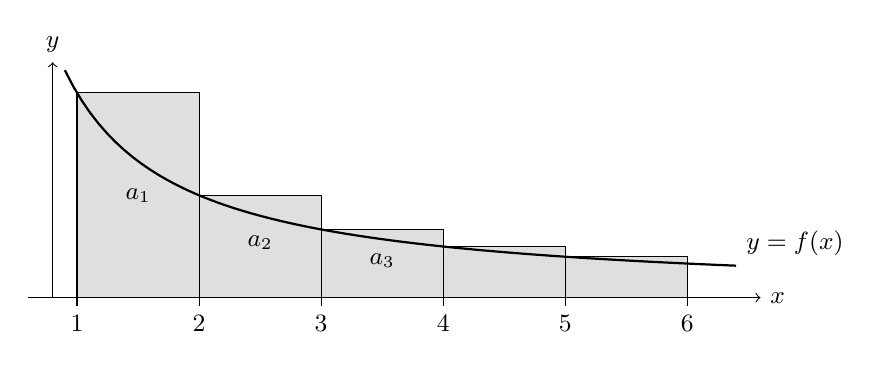
\begin{tikzpicture}[x=1.55cm,y=2.6cm,font=\small]
  \foreach \k in {1,...,5}{
    \pgfmathsetmacro{\h}{1/\k}
    \draw[fill=gray!25] (\k,0) rectangle ({\k+1},\h);
  }
  \draw[->] (0.6,0)--(6.6,0) node[right]{$x$};
  \draw[->] (0.8,0)--(0.8,1.15) node[above]{$y$};
  \draw[thick,domain=0.9:6.4,samples=80] plot (\x,{1/\x}) node[above right]{$y=f(x)$};
  \foreach \k in {1,...,6}{\draw (\k,0)--(\k,-0.04) node[below]{$\k$};}
  \node at (1.5,0.5) {$a_1$}; \node at (2.5,0.27) {$a_2$}; \node at (3.5,0.18) {$a_3$};
\end{tikzpicture}
\caption{Criterio de la integral con $f(x)=1/x$. El rectángulo sobre $[k,k+1]$ tiene altura $a_k=f(k)$ y contiene la región bajo la curva en ese intervalo; por eso $\sum_{k=1}^{n}a_k\ge\int_1^{n+1}f$. Desplazando los rectángulos una unidad a la izquierda quedan por debajo de la curva, y se obtiene la otra desigualdad.}
\label{fig:criterio-integral}
\end{figure}

\begin{corolario}[Series $p$]\label{cor:series-p}
La serie $\sum_{n=1}^{\infty}\frac{1}{n^{p}}$ converge si y solo si $p>1$. Además, $\ln(n+1)\le H_n\le1+\ln n$ para todo $n\in\N$.
\end{corolario}

\begin{proof}
Si $p\le0$, el término general no tiende a~$0$. Si $p>0$, $f(x)=x^{-p}$ es positiva y decreciente, y el \cref{teo:criterio-integral} con la \cref{prop:p-infinito} da el resultado. Con $p=1$, las desigualdades del teorema son $\ln(n+1)\le H_n\le1+\ln n$.
\end{proof}

Así, la serie armónica diverge, pero muy despacio: $H_{1000}$ está entre $\ln1001\approx6{,}91$ y $1+\ln1000\approx7{,}91$. En cambio, $\sum\frac{1}{n^{2}}$ converge, y su suma es menor que $1+\int_1^\infty x^{-2}\dif x=2$ (su valor exacto, $\frac{\pi^{2}}{6}\approx1{,}645$, se obtiene con otras técnicas).

\section{Criterios del cociente y de la raíz}

\begin{teorema}[Criterio del cociente]\label{teo:cociente}
Sea $a_n>0$ con $\frac{a_{n+1}}{a_n}\to L$. Si $L<1$, $\sum a_n$ converge; si $L>1$ (incluido $L=\infty$), diverge. Si $L=1$, el criterio no decide.
\end{teorema}

\begin{teorema}[Criterio de la raíz]\label{teo:raiz}
Sea $a_n\ge0$ con $\sqrt[n]{a_n}\to L$. Si $L<1$, $\sum a_n$ converge; si $L>1$, diverge. Si $L=1$, el criterio no decide.
\end{teorema}

\begin{proof}[Demostración del \cref{teo:raiz}]
Si $L<1$, sea $r$ con $L<r<1$. Existe $N$ con $\sqrt[n]{a_n}<r$, es decir, $a_n<r^{n}$, para $n\ge N$, y la serie converge por comparación con la geométrica de razón $r$. Si $L>1$, $\sqrt[n]{a_n}>1$, es decir, $a_n>1$, para $n$ grande, y el término general no tiende a~$0$.
\end{proof}

La demostración del criterio del cociente es análoga y se pide en el \cref{eje:5-cociente-dem}. Ambos criterios comparan con una serie geométrica, y por eso no deciden en el caso $L=1$: tanto $\sum\frac1n$, divergente, como $\sum\frac{1}{n^{2}}$, convergente, tienen $L=1$. Son especialmente útiles con factoriales y potencias $n$-ésimas.

\begin{ejemplo}\label{ej:cociente}
Para $a_n=\frac{n^{2}}{2^{n}}$, $\frac{a_{n+1}}{a_n}=\frac{(n+1)^{2}}{2n^{2}}\to\frac12<1$, y la serie converge. Para $a_n=\frac{x^{n}}{n!}$ con $x>0$, $\frac{a_{n+1}}{a_n}=\frac{x}{n+1}\to0$, y la serie converge para todo $x>0$; en el \cref{tema:6} se verá que su suma es $e^{x}-1$ (sumando desde $n=1$).
\end{ejemplo}

\section{Series alternadas y convergencia absoluta}

\begin{definicion}[Convergencia absoluta y condicional]\label{def:absoluta}
La serie $\sum a_n$ converge \emph{absolutamente} si $\sum\abs{a_n}$ converge. Si $\sum a_n$ converge pero $\sum\abs{a_n}$ diverge, converge \emph{condicionalmente}.
\end{definicion}

\begin{teorema}\label{teo:absoluta-series}
Toda serie absolutamente convergente es convergente, y $\bigl|\sum a_n\bigr|\le\sum\abs{a_n}$.
\end{teorema}

\begin{proof}
Se cumple $0\le a_n+\abs{a_n}\le2\abs{a_n}$, luego $\sum(a_n+\abs{a_n})$ converge por comparación, y $\sum a_n=\sum(a_n+\abs{a_n})-\sum\abs{a_n}$ es diferencia de dos series convergentes. La desigualdad se obtiene en el límite de $\bigl|\sum_{k\le n}a_k\bigr|\le\sum_{k\le n}\abs{a_k}$.
\end{proof}

\begin{teorema}[Criterio de Leibniz]\label{teo:leibniz}
Sea $(b_n)$ decreciente con $b_n\to0$ (luego $b_n\ge0$). La serie alternada $\sum_{n=1}^{\infty}(-1)^{n+1}b_n=b_1-b_2+b_3-\cdots$ converge, y su suma $S$ cumple $\abs{S-S_n}\le b_{n+1}$ para todo $n$.
\end{teorema}

\begin{proof}
Las sumas parciales pares cumplen $S_{2n+2}=S_{2n}+(b_{2n+1}-b_{2n+2})\ge S_{2n}$, luego son crecientes. Las impares cumplen $S_{2n+1}=S_{2n-1}-(b_{2n}-b_{2n+1})\le S_{2n-1}$, luego son decrecientes. Además $S_{2n}=S_{2n-1}-b_{2n}\le S_{2n-1}\le S_1$, así que las pares están acotadas superiormente por $S_1$, y análogamente las impares están acotadas inferiormente por $S_2$. Por el \cref{teo:monotona-acotada}, $S_{2n}\to A$ y $S_{2n+1}\to B$, y $B-A=\lim(S_{2n+1}-S_{2n})=\lim b_{2n+1}=0$. Luego $S_n\to S=A=B$. Por último, $S$ está entre dos sumas parciales consecutivas cualesquiera $S_n$ y $S_{n+1}$, de modo que $\abs{S-S_n}\le\abs{S_{n+1}-S_n}=b_{n+1}$.
\end{proof}

\begin{ejemplo}[Serie armónica alternada]\label{ej:armonica-alternada}
La serie $1-\frac12+\frac13-\frac14+\cdots$ converge por el \cref{teo:leibniz}, pero no absolutamente (\cref{teo:armonica}): converge condicionalmente. En el \cref{tema:6} se demostrará que su suma es $\ln2$. Por la cota del error, $S_{999}$ aproxima $\ln2$ con error no mayor que $b_{1000}=10^{-3}$.
\end{ejemplo}

\begin{observacion}[Reordenaciones]
Una serie absolutamente convergente puede sumarse en cualquier orden con el mismo resultado. Con una serie condicionalmente convergente no ocurre así: un teorema de Riemann afirma que sus términos pueden reordenarse para obtener cualquier suma prefijada~\cite[cap.~23]{spivak}. El ejercicio~25 de la §10.3 de Strang~\cite{strang} muestra una reordenación de la serie armónica alternada cuya suma es $\frac12\ln2$.
\end{observacion}

\begin{observacion}[Errores frecuentes]\label{obs:5-errores}
(a) Deducir la convergencia de $a_n\to0$; la serie armónica es el contraejemplo. (b) Confundir la sucesión $(a_n)$ con la serie $\sum a_n$: $\frac{n}{n+1}\to1$, luego la sucesión converge y la serie diverge. (c) Aplicar el criterio de comparación o el de la integral a series con términos negativos, o el de la integral a una función no decreciente. (d) Concluir algo del criterio del cociente cuando $L=1$. (e) Olvidar que la fórmula de la serie geométrica empieza en $n=0$: $\sum_{n=1}^{\infty}r^{n}=\frac{r}{1-r}$.
\end{observacion}

\begin{observacion}[Conexión con el curso]
En el módulo~21, el retorno descontado $G_t=\sum_{k=0}^{\infty}\gamma^{k}R_{t+k+1}$ es una serie, y si $\abs{R}\le R_{\max}$ converge absolutamente por comparación con la geométrica, con $\abs{G_t}\le\frac{R_{\max}}{1-\gamma}$. En el módulo~7, la media exponencial de Adam con gradiente constante vale $(1-\beta^{k})g$, una suma geométrica finita, y las condiciones de Robbins--Monro sobre las tasas de aprendizaje, $\sum\eta_t=\infty$ y $\sum\eta_t^{2}<\infty$, las cumple $\eta_t=\frac1t$ precisamente por el \cref{cor:series-p}; las cotas $\sum_{t\le T}\frac1t\le1+\ln T$ que se usan allí son las del \cref{teo:criterio-integral}. En el módulo~6, la entropía de una distribución geométrica es la suma de la serie $\sum k\,2^{-k}$, que se calcula en el \cref{tema:6}.
\end{observacion}

\begin{lecturas}
\item Spivak~\cite{spivak}, cap.~22 «Infinite Sequences» y cap.~23 «Infinite Series».
\item Apostol~\cite{apostol}, cap.~10 «Sequences, Infinite Series, and Improper Integrals».
\item OpenStax~\cite{openstax2}, §5.1 «Sequences», §5.2 «Infinite Series», §5.3 «The Divergence and Integral Tests», §5.4 «Comparison Tests», §5.5 «Alternating Series» y §5.6 «Ratio and Root Tests».
\item Strang~\cite{strang}, §10.1 «The Geometric Series», §10.2 «Convergence Tests: Positive Series» y §10.3 «Convergence Tests: All Series».
\item MIT 18.01SC~\cite{mit1801}, unidad~5, parte~B, sesiones~94 «Infinite Series» y~95 «Series Comparison».
\end{lecturas}

\section*{Ejercicios del tema 5}
\addcontentsline{toc}{section}{Ejercicios del tema 5}

\begin{ejercicio}{1}{eje:5-vf}
Justifique si son verdaderas o falsas: (a) si $a_n\to0$, $\sum a_n$ converge; (b) si $\sum a_n$ converge, $a_n\to0$; (c) la sucesión $a_n=\ln\bigl(1+\frac1n\bigr)$ converge y la serie $\sum a_n$ también; (d) si $\sum\abs{a_n}$ converge, $\sum a_n$ converge; (e) si $\frac{a_{n+1}}{a_n}\to1$, la serie diverge.
\end{ejercicio}

\begin{ejercicio}{2}{eje:5-limites}
Calcule los límites: (a) $\frac{3n^{2}+1}{2n^{2}-n}$; (b) $\sqrt{n+1}-\sqrt{n}$; (c) $\frac{n}{2^{n}}$; (d) $\frac{\sin n}{n}$; (e) $\bigl(1+\frac2n\bigr)^{n}$ (puede usar que $\frac{\ln(1+x)}{x}\to1$ cuando $x\to0$).
\end{ejercicio}

\begin{ejercicio}{2}{eje:5-geometricas}
(a) Sume $\frac13+\frac19+\frac{1}{27}+\cdots$ y $1-\frac14+\frac{1}{16}-\cdots$. (b) Sume $\sum_{k=2}^{\infty}3\bigl(-\frac25\bigr)^{k}$. (c) Escriba $0{,}878787\ldots$ y $0{,}123123\ldots$ como series geométricas y como fracciones irreducibles.
\fuente{adaptado de Strang~\cite{strang}, §10.1, ejercicios 3 y~13.}
\end{ejercicio}

\begin{ejercicio}{2}{eje:5-pelota}
Una pelota se deja caer desde 10~m y, tras cada bote, sube hasta $\frac35$ de la altura desde la que cayó. Calcule la distancia vertical total que recorre. Si cada caída desde altura $h$ dura $\sqrt{2h/g}$, ¿es finito el tiempo total?
\fuente{adaptado de Strang~\cite{strang}, §10.1, ejercicio~2.}
\end{ejercicio}

\begin{ejercicio}{2}{eje:5-comparacion}
Estudie la convergencia por comparación directa o en el límite: (a) $\sum\frac{1}{n^{2}+10}$; (b) $\sum\frac{1}{2n-1}$; (c) $\sum\frac{n+1}{n^{3}+2}$; (d) $\sum\frac{1}{\sqrt{n^{2}+n}}$; (e) $\sum\sin\frac{1}{n^{2}}$.
\fuente{adaptado de Strang~\cite{strang}, §10.2, ejercicio~11.}
\end{ejercicio}

\begin{ejercicio}{2}{eje:5-cociente}
Estudie la convergencia con el criterio del cociente o de la raíz: (a) $\sum\frac{3^{n}}{n!}$; (b) $\sum\frac{n!}{n^{n}}$; (c) $\sum\frac{2^{n}}{n^{2}}$; (d) $\sum\bigl(\frac{n}{2n+1}\bigr)^{n}$; (e) $\sum\frac{1}{n^{3}}$ (¿qué ocurre?).
\fuente{adaptado de Strang~\cite{strang}, §10.2, ejercicios 21 y~28.}
\end{ejercicio}

\begin{ejercicio}{2}{eje:5-integral}
Use el criterio de la integral: (a) $\sum_{n\ge1}e^{-n}$ (compruebe sumándola como geométrica); (b) $\sum_{n\ge1}n\,e^{-n}$; (c) $\sum_{n\ge2}\frac{\ln n}{n}$; (d) $\sum_{n\ge2}\frac{1}{n(\ln n)^{2}}$.
\fuente{adaptado de Strang~\cite{strang}, §10.2, ejercicios 33, 34 y~38.}
\end{ejercicio}

\begin{ejercicio}{2}{eje:5-armonica}
(a) Con las cotas del \cref{cor:series-p}, demuestre que hacen falta más de 400 términos para que $H_n>7$, y que con $1097$ términos ya se supera. (b) Admitiendo que $H_n-\ln n$ decrece hacia la constante de Euler $\gamma\approx0{,}5772$, estime el primer $n$ con $H_n>7$.
\fuente{adaptado de Strang~\cite{strang}, §10.2, ejercicio~44.}
\end{ejercicio}

\begin{ejercicio}{2}{eje:5-alternadas}
Decida si convergen absolutamente, condicionalmente o no convergen: (a) $\sum\frac{(-1)^{n+1}}{n!}$; (b) $\sum\frac{(-1)^{n+1}3^{n}}{n!}$; (c) $\sum\frac{(-1)^{n+1}n^{2}}{1+n^{4}}$; (d) $\sum\frac{(-1)^{n}}{\sqrt n}$; (e) $\sum\frac{(-1)^{n}n}{n+1}$.
\fuente{adaptado de Strang~\cite{strang}, §10.3, ejercicios 3, 4 y~9.}
\end{ejercicio}

\begin{ejercicio}{2}{eje:5-error-alternada}
(a) Acote $\abs{S_5-\ln2}$ para la serie armónica alternada, sabiendo que su suma es $\ln2$, y compare con el error real. (b) ¿Cuántos términos de $\sum\frac{(-1)^{n+1}}{n^{2}}$ garantizan, por el \cref{teo:leibniz}, un error menor que $10^{-3}$?
\fuente{adaptado de Strang~\cite{strang}, §10.3, ejercicios 18 y~20.}
\end{ejercicio}

\begin{ejercicio}{2}{eje:5-descuento}
(a) Calcule el retorno descontado $G=\sum_{k=0}^{\infty}\gamma^{k}R_{k+1}$ con $\gamma=0{,}9$ si $R_k=1$ para todo $k$, y si $R_k=1$ solo para $k$ impar y $0$ para $k$ par. (b) En Adam, la media exponencial de un gradiente constante $g$ tras $k$ pasos es $(1-\beta^{k})g$. ¿Cuántos pasos hacen falta para que $1-\beta^{k}\ge0{,}99$ con $\beta=0{,}9$? ¿Y con $\beta=0{,}999$?
\end{ejercicio}

\begin{ejercicio}{3}{eje:5-armonica-dem}
(a) Demuestre que $H_{2n}-H_n\ge\frac12$ para todo $n\in\N$. (b) Deduzca, sin usar el \cref{teo:armonica}, que $(H_n)$ no está acotada. (c) Demuestre que si $\sum a_n$ converge, entonces $\sum_{k=n+1}^{2n}a_k\to0$, y obtenga una tercera prueba de la divergencia de la serie armónica.
\end{ejercicio}

\begin{ejercicio}{3}{eje:5-cociente-dem}
Demuestre el \cref{teo:cociente}. (Indicación: si $L<1$, fije $r\in(L,1)$ y pruebe por inducción que $a_{N+m}\le a_N\,r^{m}$ a partir de cierto $N$.)
\end{ejercicio}

\begin{ejercicio}{3}{eje:5-resto}
Sea $f$ positiva y decreciente en $[1,\infty)$ con $\int_1^{\infty}f$ convergente, y sea $R_n=\sum_{k=n+1}^{\infty}f(k)$ el resto de la serie. (a) Demuestre que $\int_{n+1}^{\infty}f\le R_n\le\int_n^{\infty}f$. (b) Para $f(x)=1/x^{2}$, deduzca que $\frac{1}{n+1}\le R_n\le\frac1n$ y estime $\sum_{k=1}^{\infty}\frac{1}{k^{2}}$ a partir de $S_{10}$, con una cota del error.
\end{ejercicio}

\begin{ejercicio}{3}{eje:5-euler}
Sea $c_n=H_n-\ln n$. Demuestre que $(c_n)$ es decreciente y que $c_n>0$ para todo $n$, y concluya que converge. (Indicación: $c_n-c_{n+1}=\int_n^{n+1}\frac{\dif x}{x}-\frac{1}{n+1}$.) Su límite es la constante de Euler, $\gamma\approx0{,}5772$.
\end{ejercicio}

\begin{ejercicio}{3}{eje:5-heron}
Sea $a_1=2$ y $a_{n+1}=\frac12\bigl(a_n+\frac{2}{a_n}\bigr)$. Demuestre que $a_n\ge\sqrt2$ para todo $n$ (use la desigualdad entre las medias aritmética y geométrica), que $(a_n)$ es decreciente y que converge a $\sqrt2$. Calcule $a_2$, $a_3$ y $a_4$ y compare con $\sqrt2$.
\end{ejercicio}

% =====================================================================
\chapter{Series de potencias y series de Taylor}
\label{tema:6}
% =====================================================================

Una serie de potencias es un «polinomio de grado infinito». Dentro de su intervalo de convergencia se comporta como un polinomio: puede derivarse e integrarse término a término. Las funciones elementales $e^{x}$, $\sin x$, $\cos x$, $\ln(1+x)$ y $(1+x)^{a}$ son sumas de series de potencias, sus series de Taylor, y esa representación permite calcularlas con la precisión deseada, obtener límites y definir el número $e$. Este tema estudia el radio de convergencia, las operaciones con series y los desarrollos fundamentales, con demostración de que convergen a la función. Se siguen los capítulos~20 y~24 de Spivak~\cite{spivak}, los capítulos~7 y~11 de Apostol~\cite{apostol}, las §6.1 a~6.4 de~\cite{openstax2}, las §10.4 y~10.5 de Strang~\cite{strang} y las sesiones~97 a~100 del curso 18.01SC~\cite{mit1801}.

\section{Series de potencias y radio de convergencia}

\begin{definicion}[Serie de potencias]\label{def:serie-potencias}
Una \emph{serie de potencias} centrada en $c\in\R$ es una serie de la forma $\sum_{n=0}^{\infty}a_n(x-c)^{n}$, donde $(a_n)$ es una sucesión de números reales y $x$ es una variable real. Su \emph{dominio de convergencia} es el conjunto de los $x$ para los que converge.
\end{definicion}

Toda serie de potencias converge en $x=c$, donde vale $a_0$. El resultado siguiente muestra que el dominio de convergencia es siempre un intervalo centrado en $c$.

\begin{lema}[Lema de Abel]\label{lem:abel}
Si $\sum a_n(x_0-c)^{n}$ converge para algún $x_0\neq c$, entonces $\sum a_n(x-c)^{n}$ converge absolutamente para todo $x$ con $\abs{x-c}<\abs{x_0-c}$.
\end{lema}

\begin{proof}
Por la \cref{prop:condicion-necesaria}, $a_n(x_0-c)^{n}\to0$, y en particular existe $M$ con $\abs{a_n(x_0-c)^{n}}\le M$ para todo $n$. Sea $r=\frac{\abs{x-c}}{\abs{x_0-c}}<1$. Entonces $\abs{a_n(x-c)^{n}}=\abs{a_n(x_0-c)^{n}}\,r^{n}\le M\,r^{n}$, y la serie de valores absolutos converge por comparación con la serie geométrica $\sum Mr^{n}$.
\end{proof}

\begin{teorema}[Radio de convergencia]\label{teo:radio}
Para cada serie de potencias $\sum a_n(x-c)^{n}$ existe $R\in[0,\infty]$, su \emph{radio de convergencia}, tal que la serie converge absolutamente si $\abs{x-c}<R$ y diverge si $\abs{x-c}>R$. Si existe $\lim_{n\to\infty}\Bigl|\frac{a_n}{a_{n+1}}\Bigr|$ (finito o infinito), ese límite es $R$.
\end{teorema}

\begin{proof}
Sea $R$ el supremo (posiblemente $0$ o $\infty$) del conjunto de los valores $\abs{x_0-c}$ para los que la serie converge en $x_0$. Si $\abs{x-c}<R$, por la definición de supremo hay un $x_0$ de convergencia con $\abs{x-c}<\abs{x_0-c}$, y el \cref{lem:abel} da la convergencia absoluta en $x$. Si $\abs{x-c}>R$, la serie no converge en $x$, por la definición de $R$.

Para la fórmula, sea $\rho=\lim\abs{a_n/a_{n+1}}$ y sea $x\neq c$. El cociente de dos términos consecutivos de $\sum\abs{a_n(x-c)^{n}}$ es $\bigl|\frac{a_{n+1}}{a_n}\bigr|\abs{x-c}\to\frac{\abs{x-c}}{\rho}$. Por el \cref{teo:cociente}, la serie converge absolutamente si $\abs{x-c}<\rho$; si $\abs{x-c}>\rho$, el cociente tiende a un número mayor que~1, el término general no tiende a~$0$ y la serie diverge. Luego $R=\rho$.
\end{proof}

El intervalo $(c-R,c+R)$ es el \emph{intervalo de convergencia}. En los extremos $x=c\pm R$ el teorema no dice nada, y cada caso se estudia aparte con los criterios del \cref{tema:5}.

\begin{ejemplo}\label{ej:radios}
(a) $\sum_{n\ge0}x^{n}$: $R=1$, diverge en $x=\pm1$; dominio $(-1,1)$.
(b) $\sum_{n\ge1}\frac{x^{n}}{n}$: $\bigl|\frac{a_n}{a_{n+1}}\bigr|=\frac{n+1}{n}\to1$, luego $R=1$. En $x=1$ es la serie armónica, divergente; en $x=-1$ es la armónica alternada cambiada de signo, convergente. Dominio $[-1,1)$.
(c) $\sum_{n\ge0}\frac{x^{n}}{n!}$: $\bigl|\frac{a_n}{a_{n+1}}\bigr|=n+1\to\infty$, luego $R=\infty$.
(d) $\sum_{n\ge0}n!\,x^{n}$: $\bigl|\frac{a_n}{a_{n+1}}\bigr|=\frac{1}{n+1}\to0$, luego $R=0$ y solo converge en $x=0$.
\end{ejemplo}

\section{Derivación e integración término a término}

\begin{teorema}[Derivación e integración de series de potencias]\label{teo:termino-a-termino}
Sea $f(x)=\sum_{n=0}^{\infty}a_n(x-c)^{n}$ con radio de convergencia $R>0$. Las series
\[
\sum_{n=1}^{\infty}n\,a_n(x-c)^{n-1}\qquad\text{y}\qquad\sum_{n=0}^{\infty}\frac{a_n}{n+1}(x-c)^{n+1}
\]
tienen el mismo radio $R$; $f$ es derivable en $(c-R,c+R)$, con $f'$ igual a la primera serie, y $\int_c^{x}f(t)\dif t$ es igual a la segunda para todo $x$ de ese intervalo.
\end{teorema}

La demostración usa la convergencia uniforme de la serie en los intervalos cerrados contenidos en $(c-R,c+R)$ y puede consultarse en~\cite[cap.~24]{spivak} o \cite[cap.~11]{apostol}. Aplicando el teorema repetidamente, $f$ tiene derivadas de todos los órdenes en el intervalo de convergencia.

\begin{corolario}[Unicidad de los coeficientes]\label{cor:coeficientes}
Si $f(x)=\sum_{n=0}^{\infty}a_n(x-c)^{n}$ con $R>0$, entonces $a_n=\frac{f^{(n)}(c)}{n!}$ para todo $n$. En particular, dos series de potencias que coinciden en un entorno de $c$ tienen los mismos coeficientes.
\end{corolario}

\begin{proof}
Derivando $k$ veces término a término, $f^{(k)}(x)=\sum_{n\ge k}n(n-1)\cdots(n-k+1)\,a_n(x-c)^{n-k}$. En $x=c$ todos los términos con $n>k$ se anulan y queda $f^{(k)}(c)=k!\,a_k$.
\end{proof}

\begin{ejemplo}[Series obtenidas de la geométrica]\label{ej:desde-geometrica}
(a) Derivando $\frac{1}{1-x}=\sum_{n\ge0}x^{n}$ en $(-1,1)$: $\frac{1}{(1-x)^{2}}=\sum_{n\ge1}n\,x^{n-1}$.
(b) Sustituyendo $x$ por $-t$: $\frac{1}{1+t}=\sum_{n\ge0}(-1)^{n}t^{n}$ para $\abs t<1$. Integrando entre $0$ y $x$:
\[
\ln(1+x)=\sum_{n=1}^{\infty}\frac{(-1)^{n+1}}{n}x^{n}=x-\frac{x^{2}}{2}+\frac{x^{3}}{3}-\cdots,\qquad\abs x<1 .
\]
(c) Sustituyendo $x$ por $-t^{2}$ e integrando: $\arctan x=\sum_{n\ge0}\frac{(-1)^{n}}{2n+1}x^{2n+1}$ para $\abs x<1$.
\end{ejemplo}

\section{Series de Taylor}

\begin{definicion}[Serie de Taylor]\label{def:serie-taylor}
Sea $f$ con derivadas de todos los órdenes en un intervalo abierto que contiene a $c$. Su \emph{serie de Taylor} en $c$ es $\sum_{n=0}^{\infty}\frac{f^{(n)}(c)}{n!}(x-c)^{n}$. Para $c=0$ se llama también \emph{serie de Maclaurin}. La suma parcial de grado $n$ es el polinomio de Taylor $T_nf(x)$, y $R_nf(x)=f(x)-T_nf(x)$ es el \emph{resto}.
\end{definicion}

Por el \cref{cor:coeficientes}, si $f$ es suma de alguna serie de potencias centrada en $c$, esa serie es su serie de Taylor. Pero la serie de Taylor de $f$ puede converger y no tener por suma $f$ (\cref{eje:6-no-analitica}). La herramienta para decidirlo es el teorema de Taylor del módulo~0.5.

\begin{teorema}[Taylor con resto de Lagrange]\label{teo:taylor-lagrange}
Sea $f$ con $n+1$ derivadas en un intervalo abierto $I$ que contiene a $c$. Para cada $x\in I$ existe $\xi$ entre $c$ y $x$ tal que
\[
R_nf(x)=\frac{f^{(n+1)}(\xi)}{(n+1)!}(x-c)^{n+1}.
\]
\end{teorema}

\begin{proposicion}\label{prop:taylor-converge}
La serie de Taylor de $f$ en $c$ converge a $f(x)$ si y solo si $R_nf(x)\to0$ cuando $n\to\infty$.
\end{proposicion}

\begin{proof}
Las sumas parciales de la serie son $T_nf(x)=f(x)-R_nf(x)$, que tienden a $f(x)$ si y solo si $R_nf(x)\to0$.
\end{proof}

\section{Los desarrollos fundamentales}

\begin{teorema}[Exponencial]\label{teo:exp}
Para todo $x\in\R$, $\displaystyle e^{x}=\sum_{n=0}^{\infty}\frac{x^{n}}{n!}=1+x+\frac{x^{2}}{2}+\frac{x^{3}}{6}+\cdots$.
\end{teorema}

\begin{proof}
Todas las derivadas de $e^{x}$ son $e^{x}$ y valen~1 en $0$, así que la serie del enunciado es la de Taylor. Por el \cref{teo:taylor-lagrange}, $\abs{R_n(x)}=\frac{e^{\xi}\abs{x}^{n+1}}{(n+1)!}\le e^{\abs x}\frac{\abs{x}^{n+1}}{(n+1)!}$. La serie $\sum\frac{\abs{x}^{m}}{m!}$ converge (\cref{ej:cociente}), luego su término general tiende a~$0$ (\cref{prop:condicion-necesaria}), y $R_n(x)\to0$. Se concluye por la \cref{prop:taylor-converge}.
\end{proof}

Del mismo modo, como las derivadas de $\sin$ y $\cos$ son $\pm\sin$ y $\pm\cos$, acotadas por~1, sus restos cumplen $\abs{R_n(x)}\le\frac{\abs x^{n+1}}{(n+1)!}\to0$, y para todo $x\in\R$ (\cref{eje:6-seno-dem})
\[
\sin x=\sum_{n=0}^{\infty}\frac{(-1)^{n}x^{2n+1}}{(2n+1)!}=x-\frac{x^{3}}{6}+\cdots,\qquad
\cos x=\sum_{n=0}^{\infty}\frac{(-1)^{n}x^{2n}}{(2n)!}=1-\frac{x^{2}}{2}+\cdots.
\]

\begin{teorema}[Logaritmo]\label{teo:ln}
Para todo $x\in(-1,1]$, $\displaystyle\ln(1+x)=\sum_{n=1}^{\infty}\frac{(-1)^{n+1}}{n}x^{n}$. En particular, $\displaystyle\ln2=1-\frac12+\frac13-\frac14+\cdots$.
\end{teorema}

\begin{proof}
Para $t\neq-1$ y $n\in\N$, la suma geométrica finita da la identidad exacta
\[
\frac{1}{1+t}=\sum_{k=0}^{n-1}(-t)^{k}+\frac{(-t)^{n}}{1+t}.
\]
Integrando entre $0$ y $x\in(-1,1]$,
$\ln(1+x)=\sum_{k=1}^{n}\frac{(-1)^{k+1}x^{k}}{k}+E_n(x)$, con $E_n(x)=(-1)^{n}\int_0^{x}\frac{t^{n}}{1+t}\dif t$. Si $0\le x\le1$, como $1+t\ge1$, $\abs{E_n(x)}\le\int_0^{x}t^{n}\dif t=\frac{x^{n+1}}{n+1}\le\frac{1}{n+1}$. Si $-1<x<0$, para $t\in[x,0]$ se tiene $1+t\ge1+x>0$, y $\abs{E_n(x)}\le\frac{1}{1+x}\int_x^{0}\abs{t}^{n}\dif t=\frac{\abs{x}^{n+1}}{(n+1)(1+x)}$. En ambos casos $E_n(x)\to0$.
\end{proof}

La demostración cubre el extremo $x=1$, que el \cref{teo:termino-a-termino} no alcanza, y da además una cota explícita del error. La serie no sirve para $x>1$, porque allí su radio de convergencia, $R=1$, ya no la hace converger, aunque $\ln(1+x)$ esté definido.

\begin{teorema}[Serie binomial]\label{teo:binomial}
Sea $a\in\R$. Para todo $x\in(-1,1)$,
\[
(1+x)^{a}=\sum_{n=0}^{\infty}\binom{a}{n}x^{n},\qquad\binom{a}{n}=\frac{a(a-1)\cdots(a-n+1)}{n!},\quad\binom{a}{0}=1 .
\]
Si $a\in\N_0$, la serie es finita y se reduce al binomio de Newton.
\end{teorema}

Si $a\notin\N_0$, ningún coeficiente es nulo, $\bigl|\binom{a}{n}\big/\binom{a}{n+1}\bigr|=\frac{n+1}{\abs{a-n}}\to1$ y el radio es~1. La demostración de que la suma es $(1+x)^{a}$ se pide en el \cref{eje:6-binomial-dem}. Por ejemplo, con $a=\frac12$: $\sqrt{1+x}=1+\frac x2-\frac{x^{2}}{8}+\frac{x^{3}}{16}-\cdots$.

\begin{table}[h]
\centering
\small
\renewcommand{\arraystretch}{1.25}
\begin{tabular}{@{}>{$\displaystyle}l<{$}>{$\displaystyle}l<{$}>{$}l<{$}@{}}
\toprule
\text{Función} & \text{Serie de Maclaurin} & \text{Validez} \\
\midrule
\frac{1}{1-x} & \sum_{n\ge0}x^{n} & (-1,1) \\
e^{x} & \sum_{n\ge0}\frac{x^{n}}{n!} & \R \\
\sin x & \sum_{n\ge0}\frac{(-1)^{n}x^{2n+1}}{(2n+1)!} & \R \\
\cos x & \sum_{n\ge0}\frac{(-1)^{n}x^{2n}}{(2n)!} & \R \\
\ln(1+x) & \sum_{n\ge1}\frac{(-1)^{n+1}x^{n}}{n} & (-1,1] \\
\arctan x & \sum_{n\ge0}\frac{(-1)^{n}x^{2n+1}}{2n+1} & [-1,1] \\
(1+x)^{a} & \sum_{n\ge0}\binom{a}{n}x^{n} & (-1,1) \\
\bottomrule
\end{tabular}
\caption{Desarrollos fundamentales. La validez en $x=\pm1$ de la serie del arcotangente se prueba en el \cref{eje:6-arctan}.}
\label{tab:desarrollos}
\end{table}

\section{El número \texorpdfstring{$e$}{e}}

El número $e$ es la base de la exponencial, $e=e^{1}$. Por el \cref{teo:exp},
\[
e=\sum_{n=0}^{\infty}\frac{1}{n!}=1+1+\frac12+\frac16+\frac{1}{24}+\cdots\approx2{,}718281828 .
\]

\begin{proposicion}\label{prop:e-limite}
$\displaystyle\lim_{n\to\infty}\Bigl(1+\frac1n\Bigr)^{n}=e$.
\end{proposicion}

\begin{proof}
Se escribe $\bigl(1+\frac1n\bigr)^{n}=\exp\bigl(n\ln(1+\frac1n)\bigr)$. Con $h=\frac1n$, $n\ln(1+\frac1n)=\frac{\ln(1+h)-\ln1}{h}\to(\ln)'(1)=1$ cuando $h\to0$. Por la continuidad de la exponencial, el límite es $e^{1}=e$.
\end{proof}

\begin{teorema}[El número $e$ es irracional]\label{teo:e-irracional}
Sea $s_q=\sum_{k=0}^{q}\frac{1}{k!}$. Para todo $q\in\N$, $0<e-s_q<\frac{1}{q!\,q}$. En consecuencia, $e\notin\Q$.
\end{teorema}

\begin{proof}
El resto es $e-s_q=\sum_{k>q}\frac{1}{k!}>0$. Sacando factor común $\frac{1}{q!}$,
\[
e-s_q=\frac{1}{q!}\Bigl(\frac{1}{q+1}+\frac{1}{(q+1)(q+2)}+\cdots\Bigr)<\frac{1}{q!}\sum_{j=1}^{\infty}\frac{1}{(q+1)^{j}}=\frac{1}{q!}\cdot\frac{1/(q+1)}{1-1/(q+1)}=\frac{1}{q!\,q},
\]
donde la desigualdad es estricta porque $(q+1)(q+2)>(q+1)^{2}$. Supóngase ahora que $e=\frac pq$ con $p,q\in\N$. Entonces $x=q!\,(e-s_q)=q!\frac pq-\sum_{k=0}^{q}\frac{q!}{k!}$ es un entero, pues cada $\frac{q!}{k!}$ con $k\le q$ es entero y $q!\frac pq=(q-1)!\,p$. Pero $0<x<\frac1q\le1$, y no hay enteros estrictamente entre $0$ y $1$. Esta contradicción prueba que $e$ es irracional.
\end{proof}

La cota del teorema también es práctica: con $q=10$, $s_{10}$ aproxima $e$ con error menor que $\frac{1}{10!\cdot10}\approx2{,}8\cdot10^{-8}$.

\begin{observacion}[Errores frecuentes]\label{obs:6-errores}
(a) Dar el radio de convergencia como si fuera el dominio, sin estudiar los extremos. (b) Usar un desarrollo fuera de su intervalo de validez: $\ln3=\ln(1+2)$ no se obtiene sumando la serie en $x=2$, que diverge. (c) Suponer que la serie de Taylor de una función infinitamente derivable converge a la función (\cref{eje:6-no-analitica}). (d) En la serie binomial con $a$ negativo o fraccionario, olvidar los signos de los factores $(a-k)$.
\end{observacion}

\begin{observacion}[Conexión con el curso]
Los desarrollos de este tema son la base de muchas aproximaciones del curso. En el módulo~4 se usa el polinomio de Taylor de segundo orden, primeros términos de la serie de Taylor. En el módulo~6, la entropía de la distribución geométrica es $\sum_{k\ge1}k\,2^{-k}=2$ bits, suma que se obtiene del \cref{ej:desde-geometrica}(a) con $x=\frac12$ (\cref{eje:6-derivar-geom}). En el módulo~11, las bibliotecas numéricas calculan $\ln(1+x)$ y $e^{x}-1$ para $x$ pequeño con funciones específicas (\texttt{log1p}, \texttt{expm1}): restar $1$ tras redondear $1+x$ destruye las cifras significativas, mientras que los primeros términos de las series, $x-\frac{x^{2}}{2}$ y $x+\frac{x^{2}}{2}$, conservan la precisión. En el módulo~1, el límite de la softmax con temperatura cuando $T\to\infty$ se entiende con la aproximación de primer orden $e^{z_i/T}\approx1+\frac{z_i}{T}$: todos los numeradores tienden a~1 y la distribución, a la uniforme.
\end{observacion}

\begin{lecturas}
\item Spivak~\cite{spivak}, cap.~20 «Approximation by Polynomial Functions» y cap.~24 «Uniform Convergence and Power Series».
\item Apostol~\cite{apostol}, cap.~7 «Polynomial Approximations to Functions» y cap.~11 «Sequences and Series of Functions».
\item OpenStax~\cite{openstax2}, §6.1 «Power Series and Functions», §6.2 «Properties of Power Series», §6.3 «Taylor and Maclaurin Series» y §6.4 «Working with Taylor Series».
\item Strang~\cite{strang}, §10.4 «The Taylor Series for $e^x$, $\sin x$, and $\cos x$» y §10.5 «Power Series».
\item MIT 18.01SC~\cite{mit1801}, unidad~5, parte~B, sesiones~97 «Power Series», 98--99 «Taylor's Series» y~100 «Operations on Power Series».
\end{lecturas}

\section*{Ejercicios del tema 6}
\addcontentsline{toc}{section}{Ejercicios del tema 6}

\begin{ejercicio}{1}{eje:6-vf}
Justifique si son verdaderas o falsas: (a) si una serie de potencias centrada en $0$ converge en $x=3$, converge en $x=-2$; (b) si converge en $x=3$, converge en $x=-3$; (c) toda serie de potencias converge en al menos un punto; (d) la serie de Taylor de $\ln(1+x)$ en $0$ permite calcular $\ln5$.
\end{ejercicio}

\begin{ejercicio}{2}{eje:6-radio}
Halle el radio y el dominio de convergencia (estudiando los extremos): (a) $\sum_{n\ge1}\frac{x^{n}}{n^{2}}$; (b) $\sum_{n\ge1}n\,x^{n}$; (c) $\sum_{n\ge1}\frac{(x-2)^{n}}{3^{n}\,n}$; (d) $\sum_{n\ge0}\frac{(-1)^{n}x^{2n}}{4^{n}}$.
\end{ejercicio}

\begin{ejercicio}{2}{eje:6-e2x}
(a) Escriba la serie de $e^{2x}$, compruebe que sus coeficientes son $\frac{f^{(n)}(0)}{n!}$ y dé una serie cuya suma sea $e^{2}$. (b) Escriba la serie de $\sin2x$, compruebe con ella que la tercera derivada en $0$ vale $-8$ y dé una serie cuya suma sea $\sin2$.
\fuente{adaptado de Strang~\cite{strang}, §10.4, ejercicios 1 y~2.}
\end{ejercicio}

\begin{ejercicio}{2}{eje:6-taylor-basicas}
Calcule, a partir de las derivadas en $0$, las series de Maclaurin de: (a) $\frac{1}{1+x}$; (b) $\cosh x=\frac{e^{x}+e^{-x}}{2}$; (c) $\ln(1+x)$. Compruebe (b) sumando las series de $e^{x}$ y $e^{-x}$, y (c) con el \cref{teo:ln}.
\fuente{adaptado de Strang~\cite{strang}, §10.4, ejercicios 4, 6 y~8.}
\end{ejercicio}

\begin{ejercicio}{2}{eje:6-derivar-geom}
(a) Derive dos veces la serie geométrica y calcule $\sum_{n\ge1}\frac{n}{2^{n-1}}$ y $\sum_{n\ge2}\frac{n(n-1)}{2^{n-2}}$. (b) Deduzca $\sum_{k\ge1}k\,2^{-k}$ (la entropía en bits de la distribución geométrica de parámetro $\frac12$, módulo~6) y, para $0<p<1$, $\sum_{k\ge1}k(1-p)^{k-1}p$. (c) Sustituyendo $x$ por $1-x$ en la serie geométrica e integrando, obtenga la serie de $\ln x$ centrada en $1$.
\fuente{adaptado de Strang~\cite{strang}, §10.1, ejercicios 4 y~5.}
\end{ejercicio}

\begin{ejercicio}{2}{eje:6-productos}
Obtenga los primeros términos no nulos indicados, operando con series conocidas: (a) tres de $\frac{\sin x}{x}$; (b) cuatro de $e^{x}\sin x$; (c) cuatro de $e^{-x^{2}}$ y, de ahí, cuatro de $\int_0^{x}e^{-t^{2}}\dif t$.
\fuente{adaptado de Strang~\cite{strang}, §10.4, ejercicio~28.}
\end{ejercicio}

\begin{ejercicio}{2}{eje:6-limites}
Calcule con desarrollos de Taylor: (a) $\lim_{x\to0}\frac{e^{x}-1-x}{x^{2}}$; (b) $\lim_{x\to0}\frac{x-\sin x}{x^{3}}$; (c) $\lim_{x\to0}\frac{\ln(1+x)-x}{x^{2}}$; (d) $\lim_{x\to0}\frac{1-\cos x}{x^{2}}$.
\end{ejercicio}

\begin{ejercicio}{2}{eje:6-cos1}
Calcule $\cos1$ con cinco decimales correctos usando la serie de Taylor. ¿Cuántos términos hacen falta según la cota de error de las series alternadas?
\fuente{adaptado de Strang~\cite{strang}, §10.3, ejercicio~31.}
\end{ejercicio}

\begin{ejercicio}{2}{eje:6-aproximar}
(a) Escriba los cuatro primeros términos de $(1+x)^{1/2}$ y de $(1+x)^{-1/2}$, y aproxime $\sqrt{1{,}1}$. (b) Aproxime $\ln1{,}2$ con cuatro términos y acote el error con el \cref{teo:leibniz}. (c) ¿Cuántos términos de $\sum\frac{1}{k!}$ garantizan, por el \cref{teo:e-irracional}, un error menor que $10^{-6}$ en el cálculo de $e$?
\end{ejercicio}

\begin{ejercicio}{3}{eje:6-seno-dem}
Demuestre que $\sin x=\sum_{n\ge0}\frac{(-1)^{n}x^{2n+1}}{(2n+1)!}$ y $\cos x=\sum_{n\ge0}\frac{(-1)^{n}x^{2n}}{(2n)!}$ para todo $x\in\R$. Compruebe después, derivando término a término, que la derivada de la primera serie es la segunda.
\end{ejercicio}

\begin{ejercicio}{3}{eje:6-arctan}
(a) Integrando la identidad $\frac{1}{1+t^{2}}=\sum_{k=0}^{n-1}(-t^{2})^{k}+\frac{(-t^{2})^{n}}{1+t^{2}}$, demuestre que la serie del arcotangente converge a $\arctan x$ para todo $x\in[-1,1]$. (b) Deduzca la fórmula de Leibniz $\frac\pi4=1-\frac13+\frac15-\cdots$. (c) ¿Cuántos términos garantizan un error menor que $10^{-3}$ en $\frac\pi4$?
\end{ejercicio}

\begin{ejercicio}{3}{eje:6-binomial-dem}
Sea $a\in\R$ y $f(x)=\sum_{n\ge0}\binom{a}{n}x^{n}$ para $\abs{x}<1$. (a) Usando la identidad $(n+1)\binom{a}{n+1}+n\binom{a}{n}=a\binom{a}{n}$, demuestre que $(1+x)f'(x)=a\,f(x)$. (b) Demuestre que $g(x)=f(x)(1+x)^{-a}$ tiene derivada nula y concluya que $f(x)=(1+x)^{a}$.
\end{ejercicio}

\begin{ejercicio}{3}{eje:6-limite-exp}
Demuestre que $\lim_{n\to\infty}\bigl(1+\frac xn\bigr)^{n}=e^{x}$ para todo $x\in\R$, adaptando la demostración de la \cref{prop:e-limite}. Deduzca $\lim_{n\to\infty}\bigl(1-\frac1n\bigr)^{n}=\frac1e$ e interprete el resultado: si se eligen $n$ elementos al azar con reemplazamiento entre $n$, la probabilidad de que un elemento fijo no salga nunca tiende a $\frac1e\approx0{,}368$.
\end{ejercicio}

\begin{ejercicio}{3}{eje:6-no-analitica}
Sea $f(x)=e^{-1/x^{2}}$ si $x\neq0$ y $f(0)=0$. (a) Demuestre por inducción que, para $x\neq0$, $f^{(n)}(x)=P_n(1/x)\,e^{-1/x^{2}}$ con $P_n$ un polinomio. (b) Usando que $y^{k}e^{-y^{2}}\to0$ cuando $\abs y\to\infty$, demuestre que $f^{(n)}(0)=0$ para todo $n$. (c) Concluya que la serie de Taylor de $f$ en $0$ converge en todo $\R$ y que su suma solo coincide con $f$ en $x=0$.
\end{ejercicio}


\appendix
% =====================================================================
\chapter{Soluciones de los ejercicios}
\label{ap:soluciones}
% =====================================================================

Cada solución se presenta en cinco partes: datos, planteamiento, desarrollo, resultado y comprobación. En los ejercicios de demostración ($\star\star\star$), los pasos del desarrollo, leídos en orden, forman la demostración redactada tal como debería entregarse. La comprobación indica una forma independiente de verificar el resultado (con frecuencia, derivar la primitiva obtenida o comparar con un valor numérico) o señala dónde se ha usado cada hipótesis. Los valores decimales se redondean a cuatro cifras significativas salvo que se indique otra cosa.

% ---------------------------------------------------------------------
\section{Tema 1}

\begin{solucion}{eje:1-inmediatas}
\datos seis integrandos elementales.
\planteamiento linealidad de la integral indefinida y \cref{tab:inmediatas}.
\pasos
\begin{enumerate}[label=(\alph*)]
  \item $\int(2x^{4}+3x^{2}+x+8)\dif x=\frac25x^{5}+x^{3}+\frac12x^{2}+8x+C$.
  \item $\sqrt x+x^{-1/2}$ tiene primitiva $\frac23x^{3/2}+2x^{1/2}+C$ en $(0,\infty)$.
  \item $\int e^{7x}\dif x=\frac17e^{7x}+C$.
  \item Con la última fila de la tabla y $f(u)=1/u$: $\int\frac{\dif x}{3x+2}=\frac13\ln\abs{3x+2}+C$ en cada intervalo que no contenga $x=-\frac23$.
  \item $\int\sin(5x)\dif x=-\frac15\cos(5x)+C$.
  \item $\int\frac{\dif x}{1+x^{2}}=\arctan x+C$.
\end{enumerate}
\resultado las primitivas anteriores.
\comprobacion derivando: (a) $2x^{4}+3x^{2}+x+8$; (b) $x^{1/2}+x^{-1/2}$; (c) $e^{7x}$; (d) $\frac{3}{3(3x+2)}$; (e) $\sin5x$; (f) $\frac{1}{1+x^{2}}$.
\end{solucion}

\begin{solucion}{eje:1-vf}
\planteamiento contrastar cada afirmación con la \cref{prop:primitivas-constante}, la \cref{def:sumas} y la \cref{obs:1-errores}.
\pasos
\begin{enumerate}[label=(\alph*)]
  \item \textbf{Falsa.} $\R\setminus\{0\}$ no es un intervalo. $F(x)=\ln\abs x$ y $G(x)=\ln\abs x+H(x)$, con $H=0$ en $(-\infty,0)$ y $H=1$ en $(0,\infty)$, son primitivas de $1/x$ y $F-G$ no es constante.
  \item \textbf{Falsa.} $\int_0^{2\pi}\sin x\dif x=\eval{-\cos x}{0}{2\pi}=0$ (\cref{tema:2}), mientras que el área vale~4 (\cref{ej:area-seno}): la integral es un área con signo.
  \item \textbf{Verdadera.} En cada subintervalo, $m_i\le M_i$ y $\Delta x_i>0$.
  \item \textbf{Falsa.} $f(x)=x$ en $[-1,1]$ es integrable, no nula y $\int_{-1}^{1}x\dif x=0$ (\cref{prop:par-impar}).
\end{enumerate}
\resultado (a) F; (b) F; (c) V; (d) F.
\comprobacion (d) es cierta si además $f\ge0$ y $f$ es continua (\cref{eje:1-nula}).
\end{solucion}

\begin{solucion}{eje:1-sumas-x3}
\datos $f(x)=x^{3}$ en $[0,1]$; $n=4$; $\Delta x=\frac14$.
\planteamiento evaluar $f$ en los extremos izquierdos $0,\frac14,\frac12,\frac34$, en los derechos $\frac14,\dots,1$ y en los puntos medios $\frac18,\frac38,\frac58,\frac78$.
\pasos
\begin{enumerate}[label=\arabic*.]
  \item Izquierda: $\frac14\bigl(0+\frac{1}{64}+\frac{8}{64}+\frac{27}{64}\bigr)=\frac14\cdot\frac{36}{64}=\frac{9}{64}=0{,}1406$.
  \item Derecha: $\frac14\bigl(\frac{1}{64}+\frac{8}{64}+\frac{27}{64}+\frac{64}{64}\bigr)=\frac14\cdot\frac{100}{64}=\frac{25}{64}=0{,}3906$.
  \item Punto medio: $\frac14\cdot\frac{1+27+125+343}{512}=\frac14\cdot\frac{496}{512}=\frac{31}{128}=0{,}2422$.
  \item Como $f$ es creciente en $[0,1]$, el mínimo en cada subintervalo está en el extremo izquierdo y el máximo en el derecho: la suma por la izquierda es $\Lsum$ y la suma por la derecha es $\Usum$.
\end{enumerate}
\resultado $\Lsum=\frac{9}{64}$, $\Usum=\frac{25}{64}$, punto medio $\frac{31}{128}$.
\comprobacion los errores respecto a $\frac14$ son $0{,}1094$, $0{,}1406$ y $0{,}0078$: la regla del punto medio es mucho más precisa. Además $\Usum-\Lsum=\frac14\bigl(f(1)-f(0)\bigr)=\frac{16}{64}$, como predice el \cref{teo:monotona}.
\end{solucion}

\begin{solucion}{eje:1-sumas-strang}
\datos $f(x)=x^{3}$ en $[0,2]$; $\Delta x=\frac12$; puntos $0,\frac12,1,\frac32,2$.
\planteamiento $f$ es creciente: $\Lsum$ usa los extremos izquierdos y $\Usum$ los derechos.
\pasos
\begin{enumerate}[label=\arabic*.]
  \item Valores: $f=0,\ \frac18,\ 1,\ \frac{27}{8},\ 8$.
  \item $\Lsum=\frac12\bigl(0+\frac18+1+\frac{27}{8}\bigr)=\frac12\cdot\frac{36}{8}=\frac94=2{,}25$.
  \item $\Usum=\frac12\bigl(\frac18+1+\frac{27}{8}+8\bigr)=\frac12\cdot\frac{100}{8}=\frac{25}{4}=6{,}25$.
  \item Media: $\frac{2{,}25+6{,}25}{2}=4{,}25$.
\end{enumerate}
\resultado $\Lsum=2{,}25\le4\le\Usum=6{,}25$; la media, $4{,}25$, tiene error $0{,}25$, frente a $1{,}75$ y $2{,}25$.
\comprobacion la media de las dos sumas es la regla del trapecio; $\Usum-\Lsum=\frac12(8-0)=4$, de acuerdo con el \cref{teo:monotona}.
\end{solucion}

\begin{solucion}{eje:1-limite-x3}
\datos $f(x)=x^{3}$ en $[0,b]$; $x_k=\frac{kb}{n}$; $\sum_{k=1}^{n}k^{3}=\frac{n^{2}(n+1)^{2}}{4}$.
\planteamiento la suma por la derecha es $\frac bn\sum_{k=1}^{n}f(x_k)$; $f$ es continua, luego integrable, y la suma tiende a la integral (\cref{prop:sumas-riemann} y \cref{teo:continua}).
\pasos
\begin{enumerate}[label=\arabic*.]
  \item $\Rsum_n=\frac bn\sum_{k=1}^{n}\frac{k^{3}b^{3}}{n^{3}}=\frac{b^{4}}{n^{4}}\cdot\frac{n^{2}(n+1)^{2}}{4}=\frac{b^{4}}{4}\Bigl(1+\frac1n\Bigr)^{2}$.
  \item $\lim_{n\to\infty}\Rsum_n=\frac{b^{4}}{4}$.
\end{enumerate}
\resultado $\int_0^bx^{3}\dif x=\frac{b^{4}}{4}$.
\comprobacion con $b=2$ se obtiene $4$, el valor del \cref{eje:1-sumas-strang}; con $b=1$, $\frac14$.
\end{solucion}

\begin{solucion}{eje:1-limite-seno}
\datos $\Rsum_n=\frac1n\sum_{k=1}^{n}\sin\frac{kb}{n}$, $b>0$.
\planteamiento reconocer una suma de Riemann por la derecha de $g(x)=\sin(bx)$ en $[0,1]$ con la partición uniforme.
\pasos
\begin{enumerate}[label=\arabic*.]
  \item Con $x_k=\frac kn$ y $\Delta x=\frac1n$: $g(x_k)=\sin\frac{kb}{n}$, luego $\Rsum_n=\sum_{k=1}^{n}g(x_k)\Delta x$.
  \item $g$ es continua, luego integrable, y para la partición uniforme $\Usum-\Lsum\to0$ (\cref{teo:continua}); por la \cref{prop:sumas-riemann}, $\Rsum_n\to\int_0^{1}\sin(bx)\dif x$.
  \item Con la primitiva $-\frac{\cos(bx)}{b}$ y la regla de Barrow: $\int_0^{1}\sin(bx)\dif x=\frac{1-\cos b}{b}$.
\end{enumerate}
\resultado $\displaystyle\lim_{n\to\infty}\Rsum_n=\frac{1-\cos b}{b}$.
\comprobacion con $b=\pi$ el límite es $\frac2\pi\approx0{,}6366$, el valor medio de $\sin$ en $[0,\pi]$ (\cref{ej:media-seno}), como debe ser: $\Rsum_n$ es la media de $n$ valores equiespaciados del seno en $[0,\pi]$.
\end{solucion}

\begin{solucion}{eje:1-limites-sumas}
\datos dos sumas con $n$ sumandos.
\planteamiento sacar factor $\frac1n$ y escribir cada sumando como $f(\frac kn)$.
\pasos
\begin{enumerate}[label=(\alph*)]
  \item $\frac{n}{n^{2}+k^{2}}=\frac1n\cdot\frac{1}{1+(k/n)^{2}}$: suma de Riemann por la derecha de $\frac{1}{1+x^{2}}$ en $[0,1]$, que tiende a $\int_0^{1}\frac{\dif x}{1+x^{2}}=\frac\pi4$.
  \item $\frac{1}{n+k}=\frac1n\cdot\frac{1}{1+k/n}$: suma de Riemann de $\frac{1}{1+x}$ en $[0,1]$, que tiende a $\int_0^{1}\frac{\dif x}{1+x}=\ln2$.
\end{enumerate}
\resultado (a) $\frac\pi4\approx0{,}7854$; (b) $\ln2\approx0{,}6931$.
\comprobacion con $n=100$ las sumas valen $0{,}7829$ y $0{,}6907$; con $n=1000$, $0{,}7851$ y $0{,}6929$. Ambas funciones son decrecientes, y las sumas por la derecha son sumas inferiores: se acercan por debajo.
\end{solucion}

\begin{solucion}{eje:1-condicion}
\datos $f(x)=3x^{2}-\frac2x+e^{x}$ en $(0,\infty)$; $F(1)=2$.
\planteamiento hallar una primitiva y fijar la constante con la condición (\cref{prop:primitivas-constante}).
\pasos
\begin{enumerate}[label=\arabic*.]
  \item En $(0,\infty)$: $F(x)=x^{3}-2\ln x+e^{x}+C$.
  \item $F(1)=1-0+e+C=2$, luego $C=1-e$.
  \item En $\R\setminus\{0\}$, las primitivas son $x^{3}-2\ln\abs x+e^{x}+C_1$ para $x<0$ y $x^{3}-2\ln\abs x+e^{x}+C_2$ para $x>0$, con $C_1$ y $C_2$ independientes. Una condición en $x=1$ fija $C_2$ y deja libre $C_1$.
\end{enumerate}
\resultado $F(x)=x^{3}-2\ln x+e^{x}+1-e$.
\comprobacion $F'(x)=3x^{2}-\frac2x+e^{x}$ y $F(1)=1+e+1-e=2$.
\end{solucion}

\begin{solucion}{eje:1-estimar}
\datos (a) $\int_0^{1}\frac{\dif x}{1+x^{3}}$; (b) $\int_{10}^{20}\sqrt{x^{2}+1}\dif x$.
\planteamiento acotar el integrando por una función de integral conocida y aplicar la monotonía del \cref{teo:propiedades}(iii).
\pasos
\begin{enumerate}[label=(\alph*)]
  \item Para $x\in[0,1]$, $(1-x^{3})(1+x^{3})=1-x^{6}\le1$, luego $\frac{1}{1+x^{3}}\ge1-x^{3}$. Por la monotonía y el \cref{eje:1-limite-x3} con $b=1$: $\int_0^{1}\frac{\dif x}{1+x^{3}}\ge\int_0^{1}(1-x^{3})\dif x=1-\frac14=0{,}75>0{,}65$.
  \item Para todo $x$, $\sqrt{x^{2}+1}>\sqrt{x^{2}}=\abs x$. En $[10,20]$, $\int_{10}^{20}x\dif x$ es el área de un trapecio de bases $10$ y $20$ y altura $10$, es decir, $150$. Por la monotonía, $\int_{10}^{20}\sqrt{x^{2}+1}\dif x\ge150$, y la desigualdad es estricta porque la diferencia de los integrandos es continua, positiva y de integral no nula (\cref{eje:1-nula}).
\end{enumerate}
\resultado ambas estimaciones son ciertas; se usa la monotonía de la integral.
\comprobacion numéricamente, las integrales valen $0{,}8356$ y $150{,}35$.
\end{solucion}

\begin{solucion}{eje:1-exp-sumas}
\datos $f(x)=e^{x}$ en $[0,1]$; partición uniforme $x_k=\frac kn$.
\planteamiento $f$ es creciente, luego integrable (\cref{teo:monotona}) con $\Usum-\Lsum\to0$; basta calcular $\lim\Usum(f,P_n)$.
\pasos
\begin{enumerate}[label=\arabic*.]
  \item Como $f$ es creciente, $M_k=e^{k/n}$ y $\Usum_n=\frac1n\sum_{k=1}^{n}e^{k/n}$.
  \item Es una suma geométrica de razón $q=e^{1/n}$: $\sum_{k=1}^{n}q^{k}=q\frac{q^{n}-1}{q-1}=e^{1/n}\frac{e-1}{e^{1/n}-1}$.
  \item Con $h=\frac1n$: $\Usum_n=(e-1)\,e^{h}\,\frac{h}{e^{h}-1}$.
  \item Cuando $h\to0$, $e^{h}\to1$ y $\frac{e^{h}-1}{h}\to(e^{x})'\big|_{x=0}=1$. Luego $\Usum_n\to e-1$.
  \item Por el \cref{teo:monotona}, $\Usum_n-\Lsum_n=\frac1n(e-1)\to0$, y como $\Lsum_n\le\int_0^1e^x\dif x\le\Usum_n$, la integral es el límite común.
\end{enumerate}
\resultado $\int_0^{1}e^{x}\dif x=e-1\approx1{,}718$.
\comprobacion con $n=10$, $\Usum_{10}=1{,}806$, mayor que $e-1$, como debe ser una suma superior; la regla de Barrow da $\eval{e^{x}}{0}{1}=e-1$.
\end{solucion}

\begin{solucion}{eje:1-diferencia}
\datos $f(x)=x^{2}$ en $[0,b]$; $x_k=\frac{kb}{n}$.
\planteamiento como $f$ es creciente en $[0,b]$, $M_k=f(x_k)$ y $m_k=f(x_{k-1})$; la diferencia es telescópica.
\pasos
\begin{enumerate}[label=\arabic*.]
  \item $\Usum-\Lsum=\sum_{k=1}^{n}(M_k-m_k)\frac bn=\frac bn\sum_{k=1}^{n}\bigl(x_k^{2}-x_{k-1}^{2}\bigr)=\frac bn\bigl(x_n^{2}-x_0^{2}\bigr)=\frac bn\cdot b^{2}=\frac{b^{3}}{n}$.
  \item Interpretación: la diferencia es la suma de $n$ rectángulos de anchura $\frac bn$ cuyas alturas $f(x_k)-f(x_{k-1})$ suman $f(b)-f(0)=b^{2}$; desplazados horizontalmente hasta la misma columna, se apilan en un único rectángulo de base $\frac bn$ y altura $b^{2}$.
  \item Dado $\varepsilon>0$, si $n>\frac{b^{3}}{\varepsilon}$ se tiene $\Usum(f,P_n)-\Lsum(f,P_n)<\varepsilon$, y el \cref{teo:criterio} prueba que $f$ es integrable.
\end{enumerate}
\resultado $\Usum-\Lsum=\frac{b^{3}}{n}\to0$; $f$ es integrable en $[0,b]$.
\comprobacion coincide con el \cref{ej:x2}; con $b=1$ y $n=4$, $\frac{30}{64}-\frac{14}{64}=\frac{16}{64}=\frac14=\frac{b^{3}}{n}$.
\end{solucion}

\begin{solucion}{eje:1-positiva}
\datos $f$ integrable, $f\ge0$; para la segunda parte, $f\le g$ integrables.
\planteamiento acotar inferiormente las sumas inferiores y usar la linealidad.
\pasos
\begin{enumerate}[label=\arabic*.]
  \item Sea $P$ una partición. Como $f(x)\ge0$ para todo $x$, $0$ es cota inferior de $f$ en cada subintervalo, y el ínfimo, que es la mayor de las cotas inferiores, cumple $m_i\ge0$.
  \item Por tanto $\Lsum(f,P)=\sum m_i\Delta x_i\ge0$ para toda $P$, y $\int_a^bf=\sup_P\Lsum(f,P)\ge\Lsum(f,P)\ge0$.
  \item Si $f\le g$, la función $g-f$ es integrable por la linealidad (\cref{teo:propiedades}(i)) y es no negativa; por el paso~2, $\int_a^b(g-f)\ge0$.
  \item Por la linealidad, $\int_a^bg-\int_a^bf=\int_a^b(g-f)\ge0$.
\end{enumerate}
\resultado $\int_a^bf\ge0$ y $\int_a^bf\le\int_a^bg$.
\comprobacion la hipótesis $f\ge0$ se usa en el paso~1; la integrabilidad de $f$, para identificar la integral con el supremo de las sumas inferiores.
\end{solucion}

\begin{solucion}{eje:1-un-punto}
\datos $f(c)=1$ y $f(x)=0$ si $x\neq c$, en $[a,b]$.
\planteamiento probar que $\Lsum(f,P)=0$ siempre y que $\Usum(f,P)$ puede hacerse tan pequeña como se quiera; aplicar el \cref{teo:criterio}.
\pasos
\begin{enumerate}[label=\arabic*.]
  \item Todo subintervalo $[x_{i-1},x_i]$ tiene longitud positiva, luego contiene puntos distintos de $c$, en los que $f=0$. Como $f\ge0$, $m_i=0$ y $\Lsum(f,P)=0$ para toda $P$.
  \item $M_i=1$ si $c\in[x_{i-1},x_i]$ y $M_i=0$ en otro caso. El punto $c$ pertenece como mucho a dos subintervalos (dos si es un punto de la partición interior), luego $\Usum(f,P)\le2\norm{P}$.
  \item Dado $\varepsilon>0$, sea $P$ la partición uniforme con $\frac{b-a}{n}<\frac\varepsilon2$. Entonces $\Usum(f,P)-\Lsum(f,P)\le2\norm P<\varepsilon$, y $f$ es integrable.
  \item La integral está entre $\Lsum(f,P)=0$ y $\Usum(f,P)<\varepsilon$ para todo $\varepsilon>0$, luego $\int_a^bf=0$.
  \item Si $g$ es integrable y $\tilde g$ coincide con $g$ salvo en $c$, entonces $\tilde g=g+\bigl(\tilde g(c)-g(c)\bigr)f$, y por la linealidad $\int\tilde g=\int g+\bigl(\tilde g(c)-g(c)\bigr)\cdot0=\int g$.
\end{enumerate}
\resultado $f$ es integrable, $\int_a^bf=0$, y modificar una función integrable en un punto no altera su integral.
\comprobacion repitiendo el argumento con varios puntos, lo mismo vale para un número finito de modificaciones.
\end{solucion}

\begin{solucion}{eje:1-nula}
\datos $f$ continua, $f\ge0$ en $[a,b]$, $\int_a^bf=0$.
\planteamiento reducción al absurdo: si $f$ fuera positiva en un punto, lo sería en un intervalo, y la integral sería positiva.
\pasos
\begin{enumerate}[label=\arabic*.]
  \item Supóngase que existe $x_0\in[a,b]$ con $f(x_0)>0$. Por la continuidad, con $\varepsilon=f(x_0)/2$ existe $\delta>0$ tal que $f(x)>f(x_0)/2$ para todo $x\in J=[x_0-\delta,x_0+\delta]\cap[a,b]$.
  \item $J$ es un intervalo de longitud $\ell>0$ (al menos $\min\{\delta,b-a\}$).
  \item Sea $h=\frac{f(x_0)}{2}$ en $J$ y $h=0$ fuera de $J$. Entonces $0\le h\le f$ en $[a,b]$, $h$ es integrable (es constante en tres trozos) y $\int_a^bh=\frac{f(x_0)}{2}\ell>0$.
  \item Por la monotonía, $\int_a^bf\ge\int_a^bh>0$, en contra de la hipótesis. Luego $f(x)=0$ para todo $x$.
  \item Sin continuidad la conclusión falla: la función del \cref{eje:1-un-punto} es no negativa, tiene integral nula y vale~1 en $c$.
\end{enumerate}
\resultado $f\equiv0$; la continuidad es imprescindible.
\comprobacion la hipótesis $f\ge0$ se usa en el paso~3 ($h\le f$ fuera de $J$); sin ella, $f(x)=x$ en $[-1,1]$ es un contraejemplo.
\end{solucion}

\begin{solucion}{eje:1-racionales-irr}
\datos $g(x)=x$ si $x\in\Q$ y $g(x)=0$ si $x\notin\Q$, en $[0,1]$.
\planteamiento calcular $m_i$ y $M_i$ usando que racionales e irracionales son densos.
\pasos
\begin{enumerate}[label=\arabic*.]
  \item $g\ge0$ y todo subintervalo contiene irracionales, donde $g=0$: $m_i=0$ y $\Lsum(g,P)=0$ para toda $P$. Luego $\underline I=0$.
  \item En $[x_{i-1},x_i]$, $g(x)\le x\le x_i$; y hay racionales $q$ tan cerca de $x_i$ como se quiera, con $g(q)=q$. Luego $M_i=x_i$ y $\Usum(g,P)=\sum x_i\Delta x_i=\Usum(\mathrm{id},P)$, la suma superior de la identidad $\mathrm{id}(x)=x$.
  \item La identidad es creciente, luego integrable, y $\inf_P\Usum(\mathrm{id},P)=\int_0^{1}x\dif x=\frac12$ (área de un triángulo, o la \cref{prop:sumas-riemann} con $\Usum(\mathrm{id},P_n)=\frac{n+1}{2n}\to\frac12$).
  \item Por tanto $\overline I=\frac12\neq0=\underline I$, y $g$ no es integrable.
\end{enumerate}
\resultado $\underline I=0$, $\overline I=\frac12$; $g$ no es integrable.
\comprobacion como en el \cref{ej:dirichlet}, la falta de integrabilidad se debe a que $g$ oscila en todo subintervalo; aquí la oscilación $M_i-m_i=x_i$ no se hace pequeña al refinar.
\end{solucion}

% ---------------------------------------------------------------------
\section{Tema 2}

\begin{solucion}{eje:2-conceptos}
\datos $F(x)=\int_0^{x}\sqrt{1+t^{3}}\dif t$, $x\ge0$.
\planteamiento el integrando es continuo en $[0,\infty)$ (allí $1+t^{3}\ge1$); se aplica el \cref{teo:tfc1}.
\pasos
\begin{enumerate}[label=(\alph*)]
  \item $F(0)=\int_0^{0}=0$.
  \item Por el \cref{teo:tfc1}(ii), $F'(x)=\sqrt{1+x^{3}}$. Derivando con la regla de la cadena, $F''(x)=\frac{3x^{2}}{2\sqrt{1+x^{3}}}$.
  \item $F'(x)\ge1>0$: $F$ es estrictamente creciente. $F''(x)\ge0$: $F$ es convexa en $[0,\infty)$.
\end{enumerate}
\resultado $F(0)=0$, $F'=\sqrt{1+x^{3}}$, $F''=\frac{3x^{2}}{2\sqrt{1+x^{3}}}$; $F$ es creciente y convexa.
\comprobacion la primera parte del teorema fundamental da $F'$ sin conocer una primitiva elemental, que de hecho no existe.
\end{solucion}

\begin{solucion}{eje:2-error-barrow}
\datos $\int_{-1}^{1}x^{-2}\dif x$ «calculada» como $-2$.
\planteamiento revisar las hipótesis del \cref{teo:barrow}.
\pasos
\begin{enumerate}[label=\arabic*.]
  \item El integrando no está acotado en $[-1,1]$ (tiende a $+\infty$ en $0$), luego no es integrable en el sentido de Riemann.
  \item $F(x)=-\frac1x$ no está definida en $0$; no es continua en $[-1,1]$ ni primitiva de $x^{-2}$ en todo el intervalo.
  \item Si la integral existiera, sería $\ge0$ por la monotonía, porque el integrando es positivo. Un resultado negativo es imposible.
\end{enumerate}
\resultado el cálculo es erróneo: fallan la integrabilidad de $f$ y la hipótesis sobre $F$. Como integral impropia (\cref{tema:4}), $\int_0^{1}x^{-2}\dif x$ diverge, y también la integral pedida.
\comprobacion la \cref{prop:p-cero} con $p=2\ge1$ confirma la divergencia.
\end{solucion}

\begin{solucion}{eje:2-barrow}
\planteamiento buscar una primitiva en la \cref{tab:inmediatas} y aplicar la regla de Barrow.
\pasos
\begin{enumerate}[label=(\alph*)]
  \item $\int_1^{4}3x^{1/2}\dif x=\eval{2x^{3/2}}{1}{4}=2(8-1)=14$ y $\int_1^{4}2x^{-2}\dif x=\eval{-\frac2x}{1}{4}=-\frac12+2=\frac32$. Resultado: $14-\frac32=\frac{25}{2}$.
  \item $\eval{\sin x}{0}{\pi/2}=1$.
  \item $\eval{\frac{e^{2x}}{2}}{0}{1}=\frac{e^{2}-1}{2}\approx3{,}195$.
  \item $\eval{\ln(1+x)}{0}{1}=\ln2\approx0{,}6931$.
  \item Se separa en $[-1,0]$ y $[0,2]$: $\int_{-1}^{0}(-x)\dif x+\int_0^{2}x\dif x=\frac12+2=\frac52$.
\end{enumerate}
\resultado (a) $\frac{25}{2}$; (b) $1$; (c) $\frac{e^{2}-1}{2}$; (d) $\ln2$; (e) $\frac52$.
\comprobacion (e) es la suma de las áreas de dos triángulos, $\frac12\cdot1\cdot1+\frac12\cdot2\cdot2=\frac52$.
\end{solucion}

\begin{solucion}{eje:2-arco-seno}
\datos $y=\sin x$ y $y=\sin(ax)$, $a>0$.
\planteamiento un arco de $\sin(ax)$ va de un cero al siguiente: de $0$ a $\pi/a$, donde $\sin(ax)\ge0$.
\pasos
\begin{enumerate}[label=\arabic*.]
  \item $\int_0^{\pi}\sin x\dif x=\eval{-\cos x}{0}{\pi}=2$.
  \item $\int_0^{\pi/a}\sin(ax)\dif x=\eval{-\frac{\cos(ax)}{a}}{0}{\pi/a}=\frac{-\cos\pi+\cos0}{a}=\frac2a$.
\end{enumerate}
\resultado el área de un arco de $\sin x$ es $2$, y la de un arco de $\sin(ax)$ es $\frac2a$. Comprimir la gráfica horizontalmente en un factor $a$ divide el área por $a$.
\comprobacion la altura máxima no cambia y la base pasa de $\pi$ a $\pi/a$: el área debe escalar como la base.
\end{solucion}

\begin{solucion}{eje:2-parabola-eje}
\datos (a) $y=x^{2}-a$ con $a>0$ y el eje $x$; (b) $y=x^{2}$ con $y=2x+3$, y $y=\sqrt x$ con $y=x^{2}$.
\planteamiento hallar los cortes, decidir qué curva está encima y aplicar la \cref{def:area}.
\pasos
\begin{enumerate}[label=\arabic*.]
  \item (a) $x^{2}-a=0$ en $x=\pm\sqrt a$, y entre ellos $x^{2}-a<0$. Área: $\int_{-\sqrt a}^{\sqrt a}(a-x^{2})\dif x=\eval{ax-\frac{x^{3}}{3}}{-\sqrt a}{\sqrt a}=2\Bigl(a\sqrt a-\frac{a\sqrt a}{3}\Bigr)=\frac43a^{3/2}$.
  \item Con $a=4$: $\frac43\cdot8=\frac{32}{3}$.
  \item (b) $x^{2}=2x+3$ en $x=-1$ y $x=3$; en $x=0$ la recta vale $3>0$, luego está encima. Área: $\int_{-1}^{3}(2x+3-x^{2})\dif x=\eval{x^{2}+3x-\frac{x^{3}}{3}}{-1}{3}=9-\bigl(-\frac53\bigr)=\frac{32}{3}$.
  \item $\sqrt x=x^{2}$ en $x=0$ y $x=1$, y $\sqrt x\ge x^{2}$ en $[0,1]$. Área: $\int_0^{1}(\sqrt x-x^{2})\dif x=\frac23-\frac13=\frac13$.
\end{enumerate}
\resultado (a) $\frac{32}{3}$ y $\frac43a^{3/2}$; (b) $\frac{32}{3}$ y $\frac13$.
\comprobacion el área entre una parábola $y=x^{2}$ y una recta que la corta en $x_1<x_2$ vale $\frac{(x_2-x_1)^{3}}{6}$; con $x_2-x_1=4$ da $\frac{64}{6}=\frac{32}{3}$, y con $2\sqrt a$, $\frac{8a^{3/2}}{6}=\frac43a^{3/2}$.
\end{solucion}

\begin{solucion}{eje:2-derivar}
\planteamiento \cref{cor:leibniz} con integrandos continuos.
\pasos
\begin{enumerate}[label=(\alph*)]
  \item $f(u)=\sqrt u\sin u$ es continua en $[0,\infty)$ y $g(x)=x^{2}$: $F'(x)=\sqrt{x^{2}}\sin(x^{2})\cdot2x=2x\abs x\sin(x^{2})$; para $x>0$, $2x^{2}\sin(x^{2})$.
  \item $f(t)=\frac{1}{\sqrt{1-t^{2}}}$ es continua en $(-1,1)$ y $\sin x\in(-1,1)$ para $x\in(-\frac\pi2,\frac\pi2)$: $F'(x)=\frac{\cos x}{\sqrt{1-\sin^{2}x}}=\frac{\cos x}{\abs{\cos x}}=1$, pues $\cos x>0$. Como $F(0)=0$, $F(x)=x$ en ese intervalo; es decir, $\arcsin(\sin x)=x$.
  \item $F'(x)=e^{-x^{4}}\cdot2x-e^{-x^{2}}\cdot1=2x\,e^{-x^{4}}-e^{-x^{2}}$.
\end{enumerate}
\resultado (a) $2x\abs x\sin(x^{2})$; (b) $F'=1$, $F(x)=x$; (c) $2xe^{-x^{4}}-e^{-x^{2}}$.
\comprobacion en (c), $F(1)=\int_1^{1}=0$ y $F'(1)=2e^{-1}-e^{-1}=e^{-1}>0$: para $x$ algo mayor que~1 el intervalo $[x,x^{2}]$ crece y la integral se hace positiva.
\end{solucion}

\begin{solucion}{eje:2-hallar-f}
\datos (a) $\int_0^{x}f=2x(\sin x+1)$; (b) $\int_0^{x/2}f=2x(\sin x+1)$.
\planteamiento derivar ambos miembros (\cref{cor:leibniz}).
\pasos
\begin{enumerate}[label=\arabic*.]
  \item (a) $f(x)=2(\sin x+1)+2x\cos x$. En $x=\frac\pi2$: $f(\frac\pi2)=2\cdot2+\pi\cdot0=4$.
  \item (b) $f(\frac x2)\cdot\frac12=2(\sin x+1)+2x\cos x$, luego $f(\frac x2)=4(\sin x+1)+4x\cos x$.
  \item Para obtener $f(\frac\pi2)$ se toma $x=\pi$: $f(\frac\pi2)=4(0+1)+4\pi(-1)=4-4\pi$.
\end{enumerate}
\resultado (a) $f(\pi/2)=4$; (b) $f(\pi/2)=4-4\pi\approx-8{,}566$.
\comprobacion en ambos casos el miembro derecho se anula en $x=0$, como el izquierdo; si no fuera así, no existiría tal $f$.
\end{solucion}

\begin{solucion}{eje:2-valor-medio}
\planteamiento \cref{def:valor-medio} y resolver $f(c)=\bar f$.
\pasos
\begin{enumerate}[label=(\alph*)]
  \item $\bar f=\frac13\int_0^{3}x^{2}\dif x=\frac13\cdot9=3$; $c^{2}=3$ da $c=\sqrt3\approx1{,}732\in[0,3]$.
  \item $\bar f=\frac{1}{\ln2}\int_0^{\ln2}e^{x}\dif x=\frac{2-1}{\ln2}=\frac{1}{\ln2}\approx1{,}443$; $e^{c}=\frac{1}{\ln2}$ da $c=-\ln(\ln2)\approx0{,}3665\in[0;\,0{,}6931]$.
\end{enumerate}
\resultado (a) $\bar f=3$, $c=\sqrt3$; (b) $\bar f=1/\ln2$, $c=-\ln\ln2$.
\comprobacion en ambos casos $\bar f$ está entre el mínimo y el máximo de $f$: $0\le3\le9$ y $1\le1{,}443\le2$.
\end{solucion}

\begin{solucion}{eje:2-estudio-F}
\datos $F(x)=\int_1^{x}\frac{\dif t}{1+t^{2}}$.
\planteamiento \cref{teo:tfc1} para $F'$; comparación de integrandos para la cota.
\pasos
\begin{enumerate}[label=(\alph*)]
  \item El integrando es continuo en $\R$, luego $F$ está definida en todo $\R$. $F(1)=0$; para $x>1$, $F(x)>0$ (integrando positivo); para $x<1$, $F(x)=-\int_x^{1}<0$.
  \item $F'(x)=\frac{1}{1+x^{2}}>0$: estrictamente creciente, sin extremos relativos. $F''(x)=-\frac{2x}{(1+x^{2})^{2}}$, positiva si $x<0$ y negativa si $x>0$: convexa en $(-\infty,0)$, cóncava en $(0,\infty)$, con inflexión en $x=0$.
  \item Para $t\ge1$, $\frac{1}{1+t^{2}}<\frac{1}{t^{2}}$, luego $F(x)<\int_1^{x}\frac{\dif t}{t^{2}}=1-\frac1x<1$ para $x>1$.
  \item Como $\arctan'=\frac{1}{1+x^{2}}$, la regla de Barrow da $F(x)=\arctan x-\frac\pi4$. Límites: $\frac\pi2-\frac\pi4=\frac\pi4$ en $+\infty$ y $-\frac\pi2-\frac\pi4=-\frac{3\pi}{4}$ en $-\infty$. Además, $F(x)+\frac\pi4=\arctan x$ es impar: la gráfica es simétrica respecto del punto $(0,-\frac\pi4)$, que es el punto de inflexión.
\end{enumerate}
\resultado $F$ creciente en $\R$, inflexión en $(0,-\frac\pi4)$, $F(x)=\arctan x-\frac\pi4$, límites $\frac\pi4$ y $-\frac{3\pi}{4}$.
\comprobacion $\frac\pi4\approx0{,}785<1$, de acuerdo con la cota de (c).
\end{solucion}

\begin{solucion}{eje:2-limite}
\datos $f(t)=\frac{1}{\sqrt{1+t^{4}}}$, continua en $\R$.
\planteamiento (a) teorema del valor medio integral; (b) definición de derivada.
\pasos
\begin{enumerate}[label=(\alph*)]
  \item Por el \cref{teo:tvm-integral}, $\int_1^{1+h}f=f(c_h)\,h$ con $c_h$ entre $1$ y $1+h$. Entonces $\frac1h\int_1^{1+h}f=f(c_h)$, y como $c_h\to1$ y $f$ es continua, el límite es $f(1)$.
  \item $\frac1h\int_1^{1+h}f=\frac{F(1+h)-F(1)}{h}\to F'(1)=f(1)$, por el \cref{teo:tfc1}.
\end{enumerate}
\resultado $\frac{1}{\sqrt2}\approx0{,}7071$.
\comprobacion geométricamente, el área de una franja estrecha de anchura $h$ bajo la curva es aproximadamente $h\,f(1)$.
\end{solucion}

\begin{solucion}{eje:2-par-impar}
\datos $f$ continua en $\R$; $F(x)=\int_0^{x}f$, derivable con $F'=f$ (\cref{teo:tfc1}).
\planteamiento probar que una función auxiliar tiene derivada nula y vale $0$ en $0$.
\pasos
\begin{enumerate}[label=\arabic*.]
  \item (a) Sea $f$ par y $G(x)=F(x)+F(-x)$. Por la regla de la cadena, $G'(x)=f(x)-f(-x)=0$ para todo $x$.
  \item Por la \cref{prop:primitivas-constante}, $G$ es constante en $\R$, y $G(0)=2F(0)=0$. Luego $F(-x)=-F(x)$: $F$ es impar.
  \item (b) Sea $f$ impar y $H(x)=F(x)-F(-x)$. Entonces $H'(x)=f(x)+f(-x)=0$, $H$ es constante y $H(0)=0$. Luego $F(-x)=F(x)$: $F$ es par.
\end{enumerate}
\resultado si $f$ es par, $F$ es impar; si $f$ es impar, $F$ es par.
\comprobacion $f(x)=x^{2}$ (par) da $F(x)=\frac{x^{3}}{3}$ (impar); $f(x)=x$ (impar) da $F(x)=\frac{x^{2}}{2}$ (par). Como consecuencia se recupera la \cref{prop:par-impar}: $\int_{-a}^{a}f=F(a)-F(-a)$.
\end{solucion}

\begin{solucion}{eje:2-logaritmo}
\datos $L(x)=\int_1^{x}\frac{\dif t}{t}$, con $L'(x)=\frac1x$ y $L(1)=0$.
\planteamiento en cada apartado se compara la derivada de los dos miembros y se fija la constante en $x=1$.
\pasos
\begin{enumerate}[label=\arabic*.]
  \item (a) Sea $h(x)=L(1/x)+L(x)$ en $(0,\infty)$. Por la regla de la cadena, $h'(x)=\frac{1}{1/x}\cdot\bigl(-\frac{1}{x^{2}}\bigr)+\frac1x=-\frac1x+\frac1x=0$. Luego $h$ es constante, igual a $h(1)=0$, y $L(1/a)=-L(a)$.
  \item (b) Sea $P(n)$: «$L(x^{n})=n\,L(x)$ para todo $x>0$». $P(1)$ es trivial. Supóngase $P(n)$ y sea $k(x)=L(x^{n+1})-L(x^{n})-L(x)$. Entonces $k'(x)=\frac{(n+1)x^{n}}{x^{n+1}}-\frac{nx^{n-1}}{x^{n}}-\frac1x=\frac{n+1-n-1}{x}=0$, y $k(1)=0$. Luego $L(x^{n+1})=L(x^{n})+L(x)=nL(x)+L(x)=(n+1)L(x)$, que es $P(n+1)$.
  \item (c) En $[1,2]$, $\frac1t\ge\frac12$, luego $L(2)\ge\frac12>0$. Por (b), $L(2^{n})=nL(2)\ge\frac n2$. Dado $M$, sea $n>2M$; como $L$ es creciente, $L(x)\ge L(2^{n})>M$ para todo $x\ge2^{n}$. Luego $L(x)\to\infty$.
\end{enumerate}
\resultado $L(1/a)=-L(a)$, $L(a^{n})=nL(a)$ y $\lim_{x\to\infty}L(x)=\infty$.
\comprobacion con $L=\ln$: $\ln\frac12=-\ln2$ y $\ln8=3\ln2$. La cota $L(2^{n})\ge\frac n2$ es la misma que la de $H_{2^{n}}$ en el \cref{teo:armonica}: ambas comparan $\frac1t$ con escalones.
\end{solucion}

\begin{solucion}{eje:2-periodica}
\datos $f$ continua con $f(x+T)=f(x)$ para todo $x$.
\planteamiento derivar $G(a)=\int_a^{a+T}f$ respecto de $a$.
\pasos
\begin{enumerate}[label=\arabic*.]
  \item Por el \cref{cor:leibniz} con $g(a)=a+T$ y $h(a)=a$: $G'(a)=f(a+T)\cdot1-f(a)\cdot1=0$.
  \item Luego $G$ es constante en $\R$ (\cref{prop:primitivas-constante}).
  \item $\sin^{2}$ es continua y periódica de periodo $2\pi$, luego $\int_a^{a+2\pi}\sin^{2}x\dif x=\int_0^{2\pi}\sin^{2}x\dif x=\pi$.
\end{enumerate}
\resultado la integral sobre un periodo no depende de $a$; en particular vale $\pi$ para $\sin^{2}$.
\comprobacion con $a=-\pi$: $\int_{-\pi}^{\pi}\sin^{2}x\dif x=2\int_0^{\pi}\sin^{2}x\dif x=2\cdot\frac\pi2=\pi$ (\cref{prop:par-impar} y \cref{eje:3-trig}).
\end{solucion}

\begin{solucion}{eje:2-simetrica-f}
\datos $f$ continua en $[a,b]$ con $\int_a^{x}f=\int_x^{b}f$ para todo $x$.
\planteamiento derivar la identidad respecto de $x$.
\pasos
\begin{enumerate}[label=\arabic*.]
  \item Para $x\in(a,b)$, $\frac{d}{dx}\int_a^{x}f=f(x)$ y $\frac{d}{dx}\int_x^{b}f=\frac{d}{dx}\Bigl(\int_a^{b}f-\int_a^{x}f\Bigr)=-f(x)$, por el \cref{teo:tfc1}.
  \item Como las dos funciones de $x$ son iguales, sus derivadas también: $f(x)=-f(x)$, es decir, $f(x)=0$ en $(a,b)$.
  \item Por la continuidad, $f(a)=\lim_{x\to a^{+}}f(x)=0$ y, del mismo modo, $f(b)=0$.
\end{enumerate}
\resultado $f\equiv0$ en $[a,b]$.
\comprobacion la hipótesis dice que todo punto parte el área con signo en dos mitades iguales; con $x=a$ y $x=b$ se obtiene $\int_a^bf=0$, y la derivación muestra que eso solo es posible si $f$ es nula.
\end{solucion}

\begin{solucion}{eje:2-tvm-ponderado}
\datos $f,w$ continuas en $[a,b]$, $w\ge0$.
\planteamiento como en el \cref{teo:tvm-integral}, encerrar $\int fw$ entre $m\int w$ y $M\int w$.
\pasos
\begin{enumerate}[label=\arabic*.]
  \item Sea $W=\int_a^bw\ge0$. Si $W=0$, el \cref{eje:1-nula} da $w\equiv0$; ambos miembros son nulos y sirve cualquier $c$.
  \item Si $W>0$: por el teorema de Weierstrass, $f$ alcanza un mínimo $m=f(x_1)$ y un máximo $M=f(x_2)$. Como $w\ge0$, $m\,w(x)\le f(x)\,w(x)\le M\,w(x)$ para todo $x$.
  \item Integrando (monotonía y linealidad): $mW\le\int_a^bfw\le MW$, es decir, $\mu=\frac1W\int_a^bfw\in[f(x_1),f(x_2)]$.
  \item Por el teorema de los valores intermedios existe $c$ entre $x_1$ y $x_2$ con $f(c)=\mu$, y entonces $\int_a^bfw=f(c)\,W$.
  \item Si $w$ cambia de signo puede fallar: en $[-1,1]$ con $f(x)=w(x)=x$, $\int fw=\int_{-1}^{1}x^{2}\dif x=\frac23$, pero $f(c)\int w=f(c)\cdot0=0$ para todo $c$.
\end{enumerate}
\resultado existe $c\in[a,b]$ con $\int_a^bfw=f(c)\int_a^bw$; la hipótesis $w\ge0$ es necesaria.
\comprobacion con $w\equiv1$ se recupera el \cref{teo:tvm-integral}; la hipótesis $w\ge0$ se usa en el paso~2, al multiplicar las desigualdades por $w(x)$.
\end{solucion}

% ---------------------------------------------------------------------
\section{Tema 3}

\begin{solucion}{eje:3-elegir}
\planteamiento aplicar la estrategia de la sección~3.5 a cada integrando.
\pasos
\begin{enumerate}[label=(\alph*)]
  \item Cambio $u=x^{2}$: aparece $x\dif x=\frac12\dif u$. Resultado $\frac12\sin(x^{2})+C$.
  \item Por partes con $u=x$, $v'=\cos x$.
  \item Fracciones simples: $x^{2}-5x+6=(x-2)(x-3)$.
  \item Potencia impar del coseno: se aparta un $\cos x$ y se cambia $u=\sin x$.
  \item Sustitución trigonométrica $x=3\sin t$.
  \item Cambio $u=e^{x}$: queda $\int\frac{\dif u}{1+u^{2}}=\arctan(e^{x})+C$.
  \item Por partes con $u=\ln x$, $v'=x^{3}$.
  \item El numerador es la derivada del denominador: cambio $u=x^{2}+x+7$, resultado $\ln(x^{2}+x+7)+C$.
\end{enumerate}
\resultado las técnicas indicadas.
\comprobacion en (a), (f) y (h) la primitiva se comprueba derivando: $x\cos(x^{2})$, $\frac{e^{x}}{1+e^{2x}}$ y $\frac{2x+1}{x^{2}+x+7}$.
\end{solucion}

\begin{solucion}{eje:3-sustitucion}
\planteamiento identificar $u=\varphi(x)$ cuya derivada aparezca en el integrando (\cref{teo:sustitucion}).
\pasos
\begin{enumerate}[label=(\alph*)]
  \item $u=\ln x$, $\dif u=\frac{\dif x}{x}$: $\int u\dif u=\frac{(\ln x)^{2}}{2}+C$.
  \item $u=x^{2}-1$, $\dif u=2x\dif x$: $\frac12\int u^{1/2}\dif u=\frac13(x^{2}-1)^{3/2}+C$.
  \item $u=-x^{2}$, $\dif u=-2x\dif x$: $-\frac12\int e^{u}\dif u=-\frac12e^{-x^{2}}+C$.
  \item $u=\cos4x$, $\dif u=-4\sin4x\dif x$: $-\frac14\int\frac{\dif u}{u}=-\frac14\ln\abs{\cos4x}+C$.
  \item $u=x^{3}$, $\dif u=3x^{2}\dif x$: $\frac13\int\frac{\dif u}{1+u^{2}}=\frac13\arctan(x^{3})+C$.
\end{enumerate}
\resultado las primitivas anteriores.
\comprobacion por ejemplo, en (b), $\frac{d}{dx}\frac13(x^{2}-1)^{3/2}=\frac13\cdot\frac32(x^{2}-1)^{1/2}\cdot2x=x\sqrt{x^{2}-1}$; en (e), $\frac13\cdot\frac{3x^{2}}{1+x^{6}}$.
\end{solucion}

\begin{solucion}{eje:3-limites}
\planteamiento cambiar la variable y los límites a la vez (\cref{teo:sustitucion}).
\pasos
\begin{enumerate}[label=(\alph*)]
  \item $u=\ln x$: $x=1\mapsto u=0$, $x=e\mapsto u=1$. $\int_0^{1}\sqrt u\dif u=\eval{\frac23u^{3/2}}{0}{1}=\frac23$.
  \item $u=2+\cos x$, $\dif u=-\sin x\dif x$: $x=0\mapsto u=3$, $x=\pi\mapsto u=1$. $\int_3^{1}-u^{-3}\dif u=\int_1^{3}u^{-3}\dif u=\eval{-\frac{1}{2u^{2}}}{1}{3}=-\frac{1}{18}+\frac12=\frac49$.
  \item Para $0<b<1$, $x=\sin u$ con $u\in[0,\arcsin b]$, $\dif x=\cos u\dif u$ y $\sqrt{1-x^{2}}=\cos u>0$: $\int_0^{b}\frac{\dif x}{\sqrt{1-x^{2}}}=\int_0^{\arcsin b}\dif u=\arcsin b$, que tiende a $\frac\pi2$ cuando $b\to1^{-}$.
\end{enumerate}
\resultado (a) $\frac23$; (b) $\frac49$; (c) $\frac\pi2$.
\comprobacion (c) coincide con $\eval{\arcsin x}{0}{1}=\frac\pi2$; (b) es positiva, como corresponde a un integrando positivo en $(0,\pi)$.
\end{solucion}

\begin{solucion}{eje:3-partes}
\planteamiento \cref{teo:partes}; $u$ es el factor que se simplifica al derivar.
\pasos
\begin{enumerate}[label=(\alph*)]
  \item $u=x$, $v=-\cos x$: $-x\cos x+\int\cos x\dif x=-x\cos x+\sin x+C$.
  \item $u=x$, $v=\frac{e^{4x}}{4}$: $\frac{xe^{4x}}{4}-\frac{e^{4x}}{16}+C=\frac{(4x-1)e^{4x}}{16}+C$.
  \item $u=\ln x$, $v=\frac{x^{2}}{2}$: $\frac{x^{2}}{2}\ln x-\int\frac x2\dif x=\frac{x^{2}\ln x}{2}-\frac{x^{2}}{4}+C$.
  \item $u=\arctan x$, $v=x$: $x\arctan x-\int\frac{x}{1+x^{2}}\dif x=x\arctan x-\frac12\ln(1+x^{2})+C$.
  \item $u=x^{2}$, $v=e^{x}$: $x^{2}e^{x}-2\int xe^{x}\dif x=x^{2}e^{x}-2(x-1)e^{x}=(x^{2}-2x+2)e^{x}+C$, usando el \cref{ej:partes}(a).
\end{enumerate}
\resultado las primitivas anteriores.
\comprobacion derivando (e): $(2x-2)e^{x}+(x^{2}-2x+2)e^{x}=x^{2}e^{x}$; derivando (d): $\arctan x+\frac{x}{1+x^{2}}-\frac{x}{1+x^{2}}=\arctan x$.
\end{solucion}

\begin{solucion}{eje:3-ciclicas}
\planteamiento integrar dos veces por partes hasta que reaparezca la integral, y despejarla.
\pasos
\begin{enumerate}[label=\arabic*.]
  \item (a) Sea $K=\int e^{x}\cos x\dif x$. Con $u=\cos x$, $v=e^{x}$: $K=e^{x}\cos x+\int e^{x}\sin x\dif x$.
  \item Con $u=\sin x$, $v=e^{x}$: $\int e^{x}\sin x\dif x=e^{x}\sin x-K$. Luego $K=e^{x}\cos x+e^{x}\sin x-K$ y $K=\frac12e^{x}(\sin x+\cos x)+C$.
  \item (b) Sea $M=\int\cos(\ln x)\dif x$, $x>0$. Con $u=\cos(\ln x)$, $v=x$: $M=x\cos(\ln x)+\int\sin(\ln x)\dif x$.
  \item Con $u=\sin(\ln x)$, $v=x$: $\int\sin(\ln x)\dif x=x\sin(\ln x)-M$. Luego $M=\frac x2\bigl(\cos(\ln x)+\sin(\ln x)\bigr)+C$.
\end{enumerate}
\resultado (a) $\frac{e^{x}}{2}(\sin x+\cos x)+C$; (b) $\frac x2\bigl(\cos\ln x+\sin\ln x\bigr)+C$.
\comprobacion derivando (b): $\frac12(\cos\ln x+\sin\ln x)+\frac x2\bigl(-\frac{\sin\ln x}{x}+\frac{\cos\ln x}{x}\bigr)=\cos(\ln x)$. El cambio $x=e^{t}$ transforma (b) en $\int e^{t}\cos t\dif t$, que es (a).
\end{solucion}

\begin{solucion}{eje:3-fracciones}
\planteamiento \cref{prop:raices-simples} para raíces simples; coeficientes indeterminados para la raíz doble.
\pasos
\begin{enumerate}[label=(\alph*)]
  \item $A_3=\frac{1}{3-2}=1$, $A_2=\frac{1}{2-3}=-1$: $\int=\ln\abs{x-3}-\ln\abs{x-2}+C=\ln\Bigl|\frac{x-3}{x-2}\Bigr|+C$.
  \item $A_3=\frac{3}{1}=3$, $A_2=\frac{2}{-1}=-2$: $\int=3\ln\abs{x-3}-2\ln\abs{x-2}+C$.
  \item $x^{3}-x=x(x-1)(x+1)$: $A_0=\frac{1}{(-1)(1)}=-1$, $A_1=\frac{1}{1\cdot2}=\frac12$, $A_{-1}=\frac{1}{(-1)(-2)}=\frac12$: $\int=-\ln\abs x+\frac12\ln\abs{x-1}+\frac12\ln\abs{x+1}+C=\frac12\ln\abs{x^{2}-1}-\ln\abs x+C$.
  \item $\frac{3x+1}{(x-1)^{2}}=\frac{A}{x-1}+\frac{B}{(x-1)^{2}}$, es decir, $3x+1=A(x-1)+B$. En $x=1$: $B=4$; coeficiente de $x$: $A=3$. $\int=3\ln\abs{x-1}-\frac{4}{x-1}+C$.
\end{enumerate}
\resultado las primitivas anteriores.
\comprobacion recombinando (b): $\frac{3}{x-3}-\frac{2}{x-2}=\frac{3(x-2)-2(x-3)}{(x-3)(x-2)}=\frac{x}{(x-3)(x-2)}$.
\end{solucion}

\begin{solucion}{eje:3-fracciones-cuad}
\planteamiento \cref{teo:fracciones} con un factor cuadrático irreducible $x^{2}+1$.
\pasos
\begin{enumerate}[label=(\alph*)]
  \item $\frac{1}{(x-1)(x^{2}+1)}=\frac{A}{x-1}+\frac{Bx+C}{x^{2}+1}$, es decir, $1=A(x^{2}+1)+(Bx+C)(x-1)$. En $x=1$: $A=\frac12$. Coeficiente de $x^{2}$: $A+B=0$, $B=-\frac12$. Término independiente: $A-C=1$, $C=-\frac12$. Entonces
  $\int=\frac12\ln\abs{x-1}-\frac14\ln(x^{2}+1)-\frac12\arctan x+C$.
  \item $x^{4}-1=(x^{2}-1)(x^{2}+1)$ y $\frac{1}{x^{2}-1}-\frac{1}{x^{2}+1}=\frac{2}{x^{4}-1}$, luego $\frac{1}{x^{4}-1}=\frac12\cdot\frac{1}{x^{2}-1}-\frac12\cdot\frac{1}{x^{2}+1}$. Con el \cref{ej:fracciones}(a): $\int=\frac14\ln\Bigl|\frac{x-1}{x+1}\Bigr|-\frac12\arctan x+C$.
\end{enumerate}
\resultado las primitivas anteriores.
\comprobacion en (a), con $x=0$: $\frac{1}{(0-1)(0+1)}=-1$ y $\frac{1/2}{-1}+\frac{-1/2}{1}=-1$.
\end{solucion}

\begin{solucion}{eje:3-racional-impropia}
\planteamiento (a) dividir y separar la derivada del denominador; (b) completar el cuadrado.
\pasos
\begin{enumerate}[label=\arabic*.]
  \item (a) $\frac{x^{2}+1}{x^{2}+2x+2}=1-\frac{2x+1}{x^{2}+2x+2}$ y $2x+1=(2x+2)-1$, luego el integrando es $1-\frac{2x+2}{x^{2}+2x+2}+\frac{1}{(x+1)^{2}+1}$.
  \item Integrando cada término: $x-\ln(x^{2}+2x+2)+\arctan(x+1)+C$ (el denominador es siempre positivo).
  \item (b) $x^{2}+4x+13=(x+2)^{2}+9$, y con $h=2$, $s=3$: $\int\frac{\dif x}{(x+2)^{2}+9}=\frac13\arctan\frac{x+2}{3}+C$.
\end{enumerate}
\resultado (a) $x-\ln(x^{2}+2x+2)+\arctan(x+1)+C$; (b) $\frac13\arctan\frac{x+2}{3}+C$.
\comprobacion derivando (a): $1-\frac{2x+2}{x^{2}+2x+2}+\frac{1}{x^{2}+2x+2}=\frac{x^{2}+2x+2-2x-2+1}{x^{2}+2x+2}=\frac{x^{2}+1}{x^{2}+2x+2}$.
\end{solucion}

\begin{solucion}{eje:3-trig}
\planteamiento potencia impar: cambio de variable; potencias pares: fórmulas del ángulo doble.
\pasos
\begin{enumerate}[label=(\alph*)]
  \item $\sin^{3}x=(1-\cos^{2}x)\sin x$; con $u=\cos x$: $-\int(1-u^{2})\dif u=-\cos x+\frac{\cos^{3}x}{3}+C$.
  \item $\int_0^{\pi}\frac{1-\cos2x}{2}\dif x=\frac\pi2-\eval{\frac{\sin2x}{4}}{0}{\pi}=\frac\pi2$.
  \item $\cos^{4}x=\Bigl(\frac{1+\cos2x}{2}\Bigr)^{2}=\frac14\Bigl(1+2\cos2x+\frac{1+\cos4x}{2}\Bigr)=\frac38+\frac{\cos2x}{2}+\frac{\cos4x}{8}$. Luego $\int\cos^{4}x\dif x=\frac{3x}{8}+\frac{\sin2x}{4}+\frac{\sin4x}{32}+C$, y $\int_0^{\pi/2}\cos^{4}x\dif x=\frac{3\pi}{16}$.
\end{enumerate}
\resultado (a) $-\cos x+\frac13\cos^{3}x+C$; (b) $\frac\pi2$; (c) $\frac{3x}{8}+\frac{\sin2x}{4}+\frac{\sin4x}{32}+C$ y $\frac{3\pi}{16}$.
\comprobacion (c) coincide con $I_4=\frac{3\pi}{16}$ del \cref{eje:3-wallis}, pues $\int_0^{\pi/2}\cos^{n}=\int_0^{\pi/2}\sin^{n}$ (cambio $x\mapsto\frac\pi2-x$).
\end{solucion}

\begin{solucion}{eje:3-trig-sust}
\planteamiento $\sqrt{a^{2}-x^{2}}$: $x=a\sin t$; $1+x^{2}$: $x=\tan t$.
\pasos
\begin{enumerate}[label=(\alph*)]
  \item $x=a\sin t$, $t\in[-\frac\pi2,\frac\pi2]$: $\int_{-\pi/2}^{\pi/2}a\cos t\cdot a\cos t\dif t=a^{2}\int_{-\pi/2}^{\pi/2}\cos^{2}t\dif t=\frac{\pi a^{2}}{2}$.
  \item $x=\sin t$, $t\in(-\frac\pi2,\frac\pi2)$: $\int\frac{\sin^{2}t}{\cos t}\cos t\dif t=\int\sin^{2}t\dif t=\frac t2-\frac{\sin t\cos t}{2}+C=\frac12\bigl(\arcsin x-x\sqrt{1-x^{2}}\bigr)+C$.
  \item $x=\tan t$, $\dif x=(1+\tan^{2}t)\dif t$: $\int\frac{\dif t}{1+\tan^{2}t}=\int\cos^{2}t\dif t=\frac t2+\frac{\sin t\cos t}{2}+C$. Como $\sin t\cos t=\frac{\tan t}{1+\tan^{2}t}=\frac{x}{1+x^{2}}$, la primitiva es $\frac12\arctan x+\frac{x}{2(1+x^{2})}+C$.
\end{enumerate}
\resultado (a) $\frac{\pi a^{2}}{2}$; (b) $\frac12(\arcsin x-x\sqrt{1-x^{2}})+C$; (c) $\frac12\arctan x+\frac{x}{2(1+x^{2})}+C$.
\comprobacion (a) es el área de un semicírculo de radio $a$; con $a=1$ se recupera el \cref{ej:circulo}.
\end{solucion}

\begin{solucion}{eje:3-curso}
\datos (a) $a\neq0$, $\Delta>0$; (b) $n\ge2$.
\planteamiento (a) cambio lineal; (b) partes con $u=\ln x$ y paso al límite en el extremo $0$.
\pasos
\begin{enumerate}[label=\arabic*.]
  \item (a) $s=a(\Delta-u)$, $\dif s=-a\dif u$; $u=0\mapsto s=a\Delta$, $u=\Delta\mapsto s=0$: $\int_{a\Delta}^{0}e^{s}\bigl(-\frac{\dif s}{a}\bigr)=\frac1a\int_0^{a\Delta}e^{s}\dif s=\frac{e^{a\Delta}-1}{a}$.
  \item (b) Para $0<c<1$, con $u=\ln x$ y $v=\frac{x^{n}}{n}$: $\int_c^{1}x^{n-1}\ln x\dif x=\eval{\frac{x^{n}\ln x}{n}}{c}{1}-\frac1n\int_c^{1}x^{n-1}\dif x=-\frac{c^{n}\ln c}{n}-\frac{1-c^{n}}{n^{2}}$.
  \item Cuando $c\to0^{+}$, $c^{n}\ln c\to0$ y $c^{n}\to0$; el valor es $-\frac{1}{n^{2}}$.
\end{enumerate}
\resultado (a) $\frac{e^{a\Delta}-1}{a}$; (b) $-\frac{1}{n^{2}}$.
\comprobacion (a) tiende a $\Delta$ cuando $a\to0$, el valor con integrando constante~1. En (b), con $n=2$: $\int_0^{1}x\ln x\dif x=-\frac14$, negativo porque $\ln x<0$ en $(0,1)$.
\end{solucion}

\begin{solucion}{eje:3-reduccion}
\datos $a\neq0$, $n\in\N$; en (b), $b>0$.
\planteamiento (a) partes con $u=x^{n}$; (b) inducción usando (a) con $a=-1$ en $[0,b]$.
\pasos
\begin{enumerate}[label=\arabic*.]
  \item (a) Con $u=x^{n}$, $v=\frac{e^{ax}}{a}$: $\int x^{n}e^{ax}\dif x=\frac{x^{n}e^{ax}}{a}-\frac na\int x^{n-1}e^{ax}\dif x$.
  \item Con $a=1$: $J_0=e^{x}$, $J_1=xe^{x}-J_0=(x-1)e^{x}$, $J_2=x^{2}e^{x}-2J_1=(x^{2}-2x+2)e^{x}$, $J_3=x^{3}e^{x}-3J_2=(x^{3}-3x^{2}+6x-6)e^{x}+C$.
  \item (b) Sea $A_n=\int_0^{b}x^{n}e^{-x}\dif x$ y sea $P(n)$ la igualdad del enunciado. \emph{Caso base:} $A_0=1-e^{-b}=0!\,(1-e^{-b}\cdot1)$.
  \item \emph{Paso:} supóngase $P(n)$. Por (a) con $a=-1$ en forma definida, $A_{n+1}=\eval{-x^{n+1}e^{-x}}{0}{b}+(n+1)A_n=-b^{n+1}e^{-b}+(n+1)!\Bigl(1-e^{-b}\sum_{k=0}^{n}\frac{b^{k}}{k!}\Bigr)$.
  \item Como $b^{n+1}e^{-b}=(n+1)!\,e^{-b}\frac{b^{n+1}}{(n+1)!}$, se obtiene $A_{n+1}=(n+1)!\Bigl(1-e^{-b}\sum_{k=0}^{n+1}\frac{b^{k}}{k!}\Bigr)$, que es $P(n+1)$.
\end{enumerate}
\resultado $\int x^{3}e^{x}\dif x=(x^{3}-3x^{2}+6x-6)e^{x}+C$ y la fórmula de (b).
\comprobacion con $n=3$ y el intervalo $[0,1]$, (a) da $\int_0^{1}x^{3}e^{x}\dif x=(1-3+6-6)e+6=6-2e\approx0{,}5634$. En (b), cuando $b\to\infty$, $e^{-b}\sum_{k\le n}\frac{b^{k}}{k!}\to0$ y se obtiene $\int_0^{\infty}x^{n}e^{-x}\dif x=n!$, la \cref{prop:gamma-factorial}.
\end{solucion}

\begin{solucion}{eje:3-wallis}
\datos $I_n=\int_0^{\pi/2}\sin^{n}x\dif x$; $I_0=\frac\pi2$, $I_1=1$.
\planteamiento partes con $u=\sin^{n-1}x$ y $v'=\sin x$; después, inducción.
\pasos
\begin{enumerate}[label=\arabic*.]
  \item (a) Para $n\ge2$, con $v=-\cos x$: $I_n=\eval{-\sin^{n-1}x\cos x}{0}{\pi/2}+(n-1)\int_0^{\pi/2}\sin^{n-2}x\cos^{2}x\dif x$. El término de borde es nulo.
  \item Con $\cos^{2}x=1-\sin^{2}x$: $I_n=(n-1)(I_{n-2}-I_n)$, luego $nI_n=(n-1)I_{n-2}$.
  \item (b) Aplicando (a) $m$ veces hasta $I_0$ o $I_1$ se obtienen las fórmulas del enunciado (formalmente, por inducción sobre $m$). $I_4=\frac34\cdot\frac12\cdot\frac\pi2=\frac{3\pi}{16}$ e $I_5=\frac45\cdot\frac23\cdot1=\frac{8}{15}$.
  \item (c) Sea $Q(n)$: $nI_nI_{n-1}=\frac\pi2$. $Q(1)$: $1\cdot I_1I_0=\frac\pi2$. Si vale $Q(n)$, por (a), $(n+1)I_{n+1}I_n=(n+1)\cdot\frac{n}{n+1}I_{n-1}\cdot I_n=nI_nI_{n-1}=\frac\pi2$.
  \item En $[0,\frac\pi2]$, $0\le\sin x\le1$, luego $\sin^{n+1}x\le\sin^{n}x$ y, por la monotonía, $I_{n+1}\le I_n$.
\end{enumerate}
\resultado $I_n=\frac{n-1}{n}I_{n-2}$; $I_4=\frac{3\pi}{16}$, $I_5=\frac{8}{15}$; $nI_nI_{n-1}=\frac\pi2$ y $(I_n)$ decreciente.
\comprobacion $4\,I_4I_3=4\cdot\frac{3\pi}{16}\cdot\frac23=\frac\pi2$; además $I_5=0{,}533<I_4=0{,}589<I_3=0{,}667$.
\end{solucion}

\begin{solucion}{eje:3-beta}
\datos $B(m,n)=\int_0^{1}x^{m}(1-x)^{n}\dif x$, $m,n\in\N_0$.
\planteamiento inducción sobre $n$, para todos los $m$ a la vez; el paso integra por partes derivando $(1-x)^{n+1}$.
\pasos
\begin{enumerate}[label=\arabic*.]
  \item Sea $P(n)$: «$B(m,n)=\frac{m!\,n!}{(m+n+1)!}$ para todo $m\in\N_0$». \emph{Caso base:} $B(m,0)=\frac{1}{m+1}=\frac{m!\,0!}{(m+1)!}$.
  \item \emph{Paso:} supóngase $P(n)$ y sea $m\in\N_0$. Con $u=(1-x)^{n+1}$ y $v=\frac{x^{m+1}}{m+1}$:
  $B(m,n+1)=\eval{\frac{x^{m+1}(1-x)^{n+1}}{m+1}}{0}{1}+\frac{n+1}{m+1}\int_0^{1}x^{m+1}(1-x)^{n}\dif x$.
  \item El término de borde es nulo, y la integral es $B(m+1,n)$, a la que se aplica $P(n)$ con $m+1$:
  $B(m,n+1)=\frac{n+1}{m+1}\cdot\frac{(m+1)!\,n!}{(m+n+2)!}=\frac{m!\,(n+1)!}{(m+n+2)!}$, que es $P(n+1)$.
  \item Comprobación pedida: $x^{3}(1-x)^{2}=x^{3}-2x^{4}+x^{5}$, cuya integral es $\frac14-\frac25+\frac16=\frac{15-24+10}{60}=\frac{1}{60}$; la fórmula da $\frac{3!\,2!}{6!}=\frac{12}{720}=\frac{1}{60}$.
\end{enumerate}
\resultado $\int_0^{1}x^{m}(1-x)^{n}\dif x=\frac{m!\,n!}{(m+n+1)!}$.
\comprobacion la fórmula es simétrica en $m$ y $n$, como debe ser por el cambio $x\mapsto1-x$.
\end{solucion}

\begin{solucion}{eje:3-sustitucion-falsa}
\datos $I=\int_{-1}^{1}\frac{\dif x}{1+x^{2}}$; cambio $x=\varphi(t)=1/t$.
\planteamiento hacer el cálculo formal, comparar con el valor correcto y revisar las hipótesis del \cref{teo:sustitucion}.
\pasos
\begin{enumerate}[label=\arabic*.]
  \item (a) $\dif x=-\frac{\dif t}{t^{2}}$ y $\frac{1}{1+1/t^{2}}=\frac{t^{2}}{t^{2}+1}$, luego el integrando pasa a $-\frac{\dif t}{1+t^{2}}$. Los límites $x=\pm1$ corresponden a $t=\pm1$. Formalmente, $I=-\int_{-1}^{1}\frac{\dif t}{1+t^{2}}=-I$, y sería $I=0$.
  \item (b) $I=\arctan1-\arctan(-1)=\frac\pi2$.
  \item (c) El teorema exige que $\varphi$ tenga derivada continua en todo el intervalo $[\alpha,\beta]=[-1,1]$ de la variable $t$; pero $\varphi(t)=1/t$ no está definida en $t=0$. En la demostración se aplica la regla de Barrow a $F\circ\varphi$ en $[\alpha,\beta]$, que no es ni siquiera continua en $0$; ese es el paso que falla.
  \item En $\int_1^{2}\frac{\dif x}{1+x^{2}}$ se toma $t\in[\frac12,1]$, donde $\varphi(t)=1/t$ tiene derivada continua: $\int_1^{2}\frac{\dif x}{1+x^{2}}=\int_1^{1/2}\frac{-\dif t}{1+t^{2}}=\int_{1/2}^{1}\frac{\dif t}{1+t^{2}}=\frac\pi4-\arctan\frac12$.
\end{enumerate}
\resultado $I=\frac\pi2$; el cambio no es válido porque $\varphi$ no es de clase $C^{1}$ en $[-1,1]$; en $[1,2]$ sí lo es.
\comprobacion directamente, $\int_1^{2}\frac{\dif x}{1+x^{2}}=\arctan2-\frac\pi4\approx0{,}3218$, y $\frac\pi4-\arctan\frac12\approx0{,}7854-0{,}4636=0{,}3218$; ambos coinciden porque $\arctan2+\arctan\frac12=\frac\pi2$.
\end{solucion}

% ---------------------------------------------------------------------
\section{Tema 4}

\begin{solucion}{eje:4-clasificar}
\planteamiento buscar intervalos no acotados (primera especie) y puntos donde el integrando no está acotado (segunda especie).
\pasos
\begin{enumerate}[label=(\alph*)]
  \item Segunda especie en $x=0$: $\frac{1}{\sqrt x}\to\infty$.
  \item Segunda especie en el punto interior $x=1$; hay que estudiar $\int_0^{1}$ y $\int_1^{2}$ por separado.
  \item Primera especie (intervalo $[1,\infty)$); el integrando es acotado.
  \item Segunda especie en $x=\frac\pi2$: $\tan x\to\infty$.
  \item No es impropia: $\frac{\sin x}{x}\to1$ cuando $x\to0$, el integrando está acotado y, definiéndolo como~1 en $0$, es continuo en $[0,1]$.
  \item Primera especie en los dos extremos.
\end{enumerate}
\resultado impropias de segunda especie: (a), (b), (d); de primera: (c), (f); (e) no es impropia.
\comprobacion en (e), por el \cref{eje:1-un-punto}, el valor asignado en $x=0$ no afecta a la integral.
\end{solucion}

\begin{solucion}{eje:4-calcular}
\planteamiento \cref{prop:p-infinito,prop:p-cero} y cálculo directo del límite.
\pasos
\begin{enumerate}[label=(\alph*)]
  \item $p=2>1$: $\frac{1}{p-1}=1$.
  \item $p=10$: $\frac19$. Es el área bajo $y=x^{-10}$ a la derecha de $x=1$.
  \item $p=1$ en el origen: diverge ($-\ln c\to\infty$).
  \item $p=\frac12<1$: $\frac{1}{1-1/2}=2$.
  \item $\int_c^{e}\ln x\dif x=\eval{x\ln x-x}{c}{e}=(e-e)-(c\ln c-c)\to0$. Converge y vale~$0$.
  \item $\int_0^{b}xe^{-x^{2}}\dif x=\eval{-\frac12e^{-x^{2}}}{0}{b}=\frac12-\frac12e^{-b^{2}}\to\frac12$.
\end{enumerate}
\resultado (a) $1$; (b) $\frac19$; (c) diverge; (d) $2$; (e) $0$; (f) $\frac12$.
\comprobacion (e) vale $0$ porque el área negativa en $(0,1)$, que es $-1$ (\cref{ej:log-impropia}), se compensa con la positiva en $(1,e)$, que vale $\eval{x\ln x-x}{1}{e}=1$.
\end{solucion}

\begin{solucion}{eje:4-logaritmos}
\planteamiento cambios $u=\ln x$ y $u=\ln(\ln x)$, con $\dif u=\frac{\dif x}{x}$ y $\dif u=\frac{\dif x}{x\ln x}$.
\pasos
\begin{enumerate}[label=(\alph*)]
  \item $\int_2^{b}\frac{\dif x}{x\ln x}=\ln(\ln b)-\ln(\ln2)\to\infty$: diverge.
  \item $\int_2^{b}\frac{\dif x}{x(\ln x)^{2}}=\eval{-\frac{1}{\ln x}}{2}{b}=\frac{1}{\ln2}-\frac{1}{\ln b}\to\frac{1}{\ln2}\approx1{,}443$: converge.
  \item $\int_{100}^{b}\frac{\dif x}{x\ln x\ln(\ln x)}=\ln\bigl(\ln(\ln b)\bigr)-\ln\bigl(\ln(\ln100)\bigr)\to\infty$: diverge.
\end{enumerate}
\resultado (a) diverge; (b) converge a $\frac{1}{\ln2}$; (c) diverge.
\comprobacion la divergencia de (c) es lentísima: $\ln(\ln(\ln100))\approx0{,}42$, y para que la integral alcance~1 hace falta que $\ln(\ln(\ln b))\approx1{,}42$, es decir, $b\approx e^{e^{4{,}15}}$, un número de 28 cifras. Cada factor logarítmico más frena la divergencia, pero no la detiene; en cambio, un exponente $1+\varepsilon$ en el último logaritmo, como en (b), produce convergencia. No hay una frontera nítida entre ambos comportamientos.
\end{solucion}

\begin{solucion}{eje:4-comparar}
\planteamiento \cref{teo:comparacion-int,teo:comparacion-limite} con funciones $x^{-p}$.
\pasos
\begin{enumerate}[label=(\alph*)]
  \item $0<\frac{1}{x^{3}+1}\le\frac{1}{x^{3}}$ y $p=3>1$: \textbf{converge}.
  \item $\frac{2+\sin x}{x}\ge\frac1x\ge0$ y $\int_1^{\infty}\frac{\dif x}{x}$ diverge: \textbf{diverge}.
  \item $x+x^{3}\ge x$, luego $0<\frac{1}{\sqrt{x+x^{3}}}\le\frac{1}{\sqrt x}$, y $\int_0^{1}x^{-1/2}$ converge: \textbf{converge}.
  \item $\frac{1/\sqrt{x^{2}+x}}{1/x}=\frac{1}{\sqrt{1+1/x}}\to1$ y $\int_1^{\infty}\frac{\dif x}{x}$ diverge: \textbf{diverge}.
  \item $\frac{e^{x}}{x}\ge\frac1x>0$ en $(0,1]$ y $\int_0^{1}\frac{\dif x}{x}$ diverge: \textbf{diverge}.
  \item $x^{4}e^{-x}\to0$, luego $x^{2}e^{-x}\le\frac{1}{x^{2}}$ para $x\ge x_0$; en $[0,x_0]$ la integral es propia: \textbf{converge}.
\end{enumerate}
\resultado convergen (a), (c) y (f); divergen (b), (d) y (e).
\comprobacion (f) es $\Gamma(3)=2!=2$ (\cref{prop:gamma-factorial}).
\end{solucion}

\begin{solucion}{eje:4-seno}
\datos $\int_1^{N}\frac{\sin x}{x^{2}}\dif x$, $N>1$.
\planteamiento acotar el valor absoluto del integrando por $\frac{1}{x^{2}}$.
\pasos
\begin{enumerate}[label=\arabic*.]
  \item Por el \cref{teo:propiedades}(v) y la monotonía: $\int_1^{N}\frac{\sin x}{x^{2}}\dif x\le\int_1^{N}\frac{\abs{\sin x}}{x^{2}}\dif x\le\int_1^{N}\frac{\dif x}{x^{2}}=1-\frac1N<1$.
  \item $\int_1^{\infty}\frac{\abs{\sin x}}{x^{2}}$ converge por comparación con $\int_1^{\infty}x^{-2}$, y el \cref{teo:absoluta-int} da la convergencia de $\int_1^{\infty}\frac{\sin x}{x^{2}}$.
\end{enumerate}
\resultado la cota es estricta para todo $N$ y la integral impropia converge (absolutamente), con valor de módulo menor o igual que~1.
\comprobacion numéricamente, $\int_1^{\infty}\frac{\sin x}{x^{2}}\dif x\approx0{,}506$, dentro de la cota.
\end{solucion}

\begin{solucion}{eje:4-gamma-valores}
\planteamiento \cref{prop:gamma-factorial} y cambio lineal.
\pasos
\begin{enumerate}[label=\arabic*.]
  \item $\Gamma(2)=1!=1$; $\Gamma(5)=4!=24$; $\frac{\Gamma(7)}{\Gamma(5)}=\frac{6!}{4!}=6\cdot5=30$.
  \item Con $u=2x$, $x=\frac u2$, $\dif x=\frac{\dif u}{2}$: $\int_0^{\infty}x^{3}e^{-2x}\dif x=\int_0^{\infty}\frac{u^{3}}{8}e^{-u}\frac{\dif u}{2}=\frac{\Gamma(4)}{16}=\frac{6}{16}=\frac38$.
  \item En general, con $u=\lambda x$: $\int_0^{\infty}x^{n}e^{-\lambda x}\dif x=\frac{1}{\lambda^{n+1}}\int_0^{\infty}u^{n}e^{-u}\dif u=\frac{n!}{\lambda^{n+1}}$.
\end{enumerate}
\resultado $1$, $24$, $30$; $\frac38$; $\frac{n!}{\lambda^{n+1}}$.
\comprobacion con $n=0$: $\int_0^{\infty}e^{-\lambda x}\dif x=\frac1\lambda$, el \cref{ej:impropias1}(a).
\end{solucion}

\begin{solucion}{eje:4-gamma-medio}
\planteamiento cambio $x=u^{2}$ en la definición de $\Gamma(\frac12)$ y recurrencia de la \cref{prop:gamma-factorial}.
\pasos
\begin{enumerate}[label=\arabic*.]
  \item (a) En $[c,b]\subset(0,\infty)$, con $x=u^{2}$, $\dif x=2u\dif u$: $\int_c^{b}x^{-1/2}e^{-x}\dif x=\int_{\sqrt c}^{\sqrt b}\frac1ue^{-u^{2}}2u\dif u=2\int_{\sqrt c}^{\sqrt b}e^{-u^{2}}\dif u$.
  \item Pasando al límite ($c\to0^{+}$, $b\to\infty$) y usando el \cref{teo:gauss} y la paridad: $\Gamma(\frac12)=2\cdot\frac{\sqrt\pi}{2}=\sqrt\pi$.
  \item (b) $\Gamma(\frac32)=\frac12\Gamma(\frac12)=\frac{\sqrt\pi}{2}\approx0{,}8862$; $\Gamma(\frac52)=\frac32\Gamma(\frac32)=\frac{3\sqrt\pi}{4}\approx1{,}329$.
  \item En la notación $s!=\Gamma(s+1)$: $(\frac12)!=\Gamma(\frac32)=\frac{\sqrt\pi}{2}$.
\end{enumerate}
\resultado $\Gamma(\frac12)=\sqrt\pi$, $\Gamma(\frac32)=\frac{\sqrt\pi}{2}$, $\Gamma(\frac52)=\frac{3\sqrt\pi}{4}$.
\comprobacion $\Gamma(\frac32)\approx0{,}886$ está entre $\Gamma(1)=1$ y $\Gamma(2)=1$, cerca del mínimo de $\Gamma$ en $(1,2)$, que vale aproximadamente $0{,}886$.
\end{solucion}

\begin{solucion}{eje:4-erf}
\datos $E(x)=\frac{1}{\sqrt{2\pi}}\int_0^{x}e^{-u^{2}/2}\dif u$, $F(x)=\int_0^{x}e^{-t^{2}}\dif t$, $F(x)\to\frac{\sqrt\pi}{2}$.
\planteamiento cambio $u=\sqrt2\,t$.
\pasos
\begin{enumerate}[label=\arabic*.]
  \item Con $u=\sqrt2\,t$, $\dif u=\sqrt2\dif t$, el límite $x$ pasa a $x/\sqrt2$: $E(x)=\frac{\sqrt2}{\sqrt{2\pi}}\int_0^{x/\sqrt2}e^{-t^{2}}\dif t=\frac{1}{\sqrt\pi}F\bigl(\tfrac{x}{\sqrt2}\bigr)$.
  \item Cuando $x\to\infty$: $E(x)\to\frac{1}{\sqrt\pi}\cdot\frac{\sqrt\pi}{2}=\frac12$.
  \item El integrando $e^{-t^{2}}$ es par, luego $F$ es impar (\cref{eje:2-par-impar}) y $E$ también: $E(x)\to-\frac12$ cuando $x\to-\infty$.
  \item (b) Por la aditividad, $\frac{1}{\sqrt{2\pi}}\int_a^{b}e^{-u^{2}/2}\dif u=E(b)-E(a)$.
\end{enumerate}
\resultado $E(x)=\frac{1}{\sqrt\pi}F(x/\sqrt2)$; límites $\pm\frac12$; $\frac{1}{\sqrt{2\pi}}\int_a^{b}e^{-u^{2}/2}\dif u=E(b)-E(a)$.
\comprobacion $\frac{1}{\sqrt{2\pi}}\int_{-N}^{N}e^{-u^{2}/2}\dif u=E(N)-E(-N)=2E(N)\to1$: la densidad normal estándar integra~1 (\cref{cor:gauss}). La función de distribución es $\Phi(x)=\frac12+E(x)$.
\end{solucion}

\begin{solucion}{eje:4-normal}
\planteamiento integración por partes en $[-R,R]$ o $[0,b]$ y paso al límite.
\pasos
\begin{enumerate}[label=\arabic*.]
  \item (a) Con $u=x$, $v=-e^{-x^{2}/2}$: $\int_{-R}^{R}x^{2}e^{-x^{2}/2}\dif x=\eval{-xe^{-x^{2}/2}}{-R}{R}+\int_{-R}^{R}e^{-x^{2}/2}\dif x=-2Re^{-R^{2}/2}+\int_{-R}^{R}e^{-x^{2}/2}\dif x$.
  \item El integrando es par y positivo; ambas colas convergen (por comparación, $x^{2}e^{-x^{2}/2}\le\frac{1}{x^{2}}$ para $x$ grande), de modo que basta el límite simétrico. Cuando $R\to\infty$: $Re^{-R^{2}/2}\to0$ y, por el \cref{cor:gauss}, la integral vale $\sqrt{2\pi}$.
  \item Para la normal estándar, $\E[X]=\frac{1}{\sqrt{2\pi}}\int xe^{-x^{2}/2}\dif x=0$ (integrando impar y absolutamente integrable) y $\E[X^{2}]=\frac{1}{\sqrt{2\pi}}\sqrt{2\pi}=1$; luego $\operatorname{Var}(X)=1$.
  \item (b) Con $u=x$, $v=-\frac12e^{-x^{2}}$: $\int_0^{b}x^{2}e^{-x^{2}}\dif x=-\frac b2e^{-b^{2}}+\frac12\int_0^{b}e^{-x^{2}}\dif x\to\frac12\cdot\frac{\sqrt\pi}{2}=\frac{\sqrt\pi}{4}$.
\end{enumerate}
\resultado $\int_{-\infty}^{\infty}x^{2}e^{-x^{2}/2}\dif x=\sqrt{2\pi}$, varianza~1; $\int_0^{\infty}x^{2}e^{-x^{2}}\dif x=\frac{\sqrt\pi}{4}\approx0{,}4431$.
\comprobacion (b) también se obtiene de (a) con el cambio $x=t/\sqrt2$: $\int_0^{\infty}x^{2}e^{-x^{2}}\dif x=\frac{1}{2\sqrt2}\int_0^{\infty}t^{2}e^{-t^{2}/2}\dif t=\frac{1}{2\sqrt2}\cdot\frac{\sqrt{2\pi}}{2}=\frac{\sqrt\pi}{4}$.
\end{solucion}

\begin{solucion}{eje:4-gamma-conv}
\datos $s\le0$.
\planteamiento acotar inferiormente el integrando en $(0,1]$ por una función $x^{-p}$ con $p\ge1$.
\pasos
\begin{enumerate}[label=\arabic*.]
  \item En $(0,1]$, $e^{-x}\ge e^{-1}$, luego $x^{s-1}e^{-x}\ge e^{-1}x^{-(1-s)}>0$.
  \item Como $s\le0$, el exponente $p=1-s\ge1$, y $\int_0^{1}x^{-p}\dif x$ diverge (\cref{prop:p-cero}).
  \item Por el \cref{teo:comparacion-int} (en su versión para el extremo $0$), $\int_0^{1}x^{s-1}e^{-x}\dif x$ diverge, y con ella la integral en $(0,\infty)$, cuyo integrando es positivo.
  \item Junto con la convergencia para $s>0$ probada tras la \cref{def:gamma}, la integral converge si y solo si $s>0$.
\end{enumerate}
\resultado la integral que define $\Gamma(s)$ converge exactamente para $s>0$.
\comprobacion con $s=0$ el integrando es $\frac{e^{-x}}{x}\approx\frac1x$ cerca de $0$, el caso límite de la divergencia logarítmica.
\end{solucion}

\begin{solucion}{eje:4-limite-comp}
\datos $f,g>0$ en $[a,\infty)$, $\frac fg\to L\in(0,\infty)$.
\planteamiento con $\varepsilon=\frac L2$ en la definición de límite se obtienen cotas $\frac L2g\le f\le2Lg$; después se aplica el \cref{teo:comparacion-int}.
\pasos
\begin{enumerate}[label=\arabic*.]
  \item Existe $x_0\ge a$ tal que $\bigl|\frac{f(x)}{g(x)}-L\bigr|<\frac L2$ para $x\ge x_0$, es decir, $\frac L2g(x)<f(x)<\frac{3L}{2}g(x)\le2Lg(x)$.
  \item Si $\int_a^{\infty}g$ converge, también $\int_{x_0}^{\infty}2Lg$, y por comparación $\int_{x_0}^{\infty}f$ converge; $\int_a^{x_0}f$ es una integral propia, luego $\int_a^{\infty}f$ converge.
  \item Si $\int_a^{\infty}f$ converge, de $g<\frac2Lf$ en $[x_0,\infty)$ se deduce del mismo modo que $\int_a^{\infty}g$ converge.
  \item Por tanto ambas convergen o ambas divergen.
  \item Aplicaciones: $\frac{(x+1)/(x^{3}+2)}{1/x^{2}}=\frac{x^{3}+x^{2}}{x^{3}+2}\to1$ y $\int_1^{\infty}x^{-2}$ converge: la primera \textbf{converge}. Para $x\ge1$, $\sin\frac1x>0$ y $\frac{\sin(1/x)}{1/x}\to1$ (pues $\frac{\sin u}{u}\to1$ cuando $u\to0$); como $\int_1^{\infty}\frac{\dif x}{x}$ diverge, la segunda \textbf{diverge}.
\end{enumerate}
\resultado el teorema queda demostrado; la primera integral converge y la segunda diverge.
\comprobacion la hipótesis $L>0$ se usa en el paso~3 (para dividir por $L$); con $L=0$ solo vale la implicación del paso~2.
\end{solucion}

\begin{solucion}{eje:4-dirichlet}
\datos $\int_1^{\infty}\frac{\sin x}{x}\dif x$.
\planteamiento integrar por partes para pasar de $\frac1x$ a $\frac{1}{x^{2}}$, que es integrable en el infinito.
\pasos
\begin{enumerate}[label=\arabic*.]
  \item Con $u=\frac1x$, $v=-\cos x$: $\int_1^{b}\frac{\sin x}{x}\dif x=\eval{-\frac{\cos x}{x}}{1}{b}-\int_1^{b}\frac{\cos x}{x^{2}}\dif x=\cos1-\frac{\cos b}{b}-\int_1^{b}\frac{\cos x}{x^{2}}\dif x$.
  \item $\bigl|\frac{\cos b}{b}\bigr|\le\frac1b\to0$.
  \item $\bigl|\frac{\cos x}{x^{2}}\bigr|\le\frac{1}{x^{2}}$, luego $\int_1^{\infty}\frac{\cos x}{x^{2}}\dif x$ converge absolutamente (como en el \cref{ej:criterios}(b)).
  \item Los tres términos tienen límite cuando $b\to\infty$, y $\int_1^{\infty}\frac{\sin x}{x}\dif x=\cos1-\int_1^{\infty}\frac{\cos x}{x^{2}}\dif x$ converge.
  \item En $(0,1]$, $\frac{\sin x}{x}$ está acotada y tiende a~1 en $0$; definida como~1 en $x=0$ es continua en $[0,1]$, y $\int_0^{1}$ es una integral ordinaria. Luego $\int_0^{\infty}\frac{\sin x}{x}\dif x$ converge.
\end{enumerate}
\resultado la integral converge.
\comprobacion la convergencia no es absoluta: en cada $[k\pi,(k+1)\pi]$, $\int\frac{\abs{\sin x}}{x}\ge\frac{2}{(k+1)\pi}$, y la suma de estas cotas es una serie armónica, divergente (\cref{teo:armonica}). Su valor, que se obtiene con otras técnicas, es $\frac\pi2$.
\end{solucion}

\begin{solucion}{eje:4-potencias}
\datos $f(x)=(\alpha-1)x^{-\alpha}$, $x\ge1$.
\planteamiento \cref{prop:p-infinito} con exponentes $\alpha$, $\alpha-1$ y $\alpha-2$.
\pasos
\begin{enumerate}[label=\arabic*.]
  \item (a) Si $\alpha<1$, $f<0$; si $\alpha=1$, $f\equiv0$ e integra $0$. Si $\alpha>1$, $f>0$ e $\int_1^{\infty}f=(\alpha-1)\cdot\frac{1}{\alpha-1}=1$. Luego $f$ es densidad si y solo si $\alpha>1$.
  \item (b) $\int_1^{\infty}xf(x)\dif x=(\alpha-1)\int_1^{\infty}x^{-(\alpha-1)}\dif x$ converge si y solo si $\alpha-1>1$, es decir, $\alpha>2$, y vale $\frac{\alpha-1}{\alpha-2}$.
  \item (c) $\int_1^{\infty}x^{2}f(x)\dif x=(\alpha-1)\int_1^{\infty}x^{-(\alpha-2)}\dif x$ es finito si y solo si $\alpha>3$, y vale $\frac{\alpha-1}{\alpha-3}$.
\end{enumerate}
\resultado densidad si $\alpha>1$; media finita si $\alpha>2$, igual a $\frac{\alpha-1}{\alpha-2}$; segundo momento finito si $\alpha>3$.
\comprobacion con $\alpha=3{,}5$, la media es $\frac{2{,}5}{1{,}5}=\frac53$. Con $\alpha=2{,}5$ la media es finita ($3$) pero la varianza es infinita: las colas pesadas de las leyes de potencia hacen que los promedios muestrales fluctúen mucho.
\end{solucion}

\begin{solucion}{eje:4-decreciente}
\datos $f\ge0$ decreciente en $[1,\infty)$, $\int_1^{\infty}f=I$ finita.
\planteamiento acotar $\frac x2f(x)$ por una integral sobre $[\frac x2,x]$, que tiende a~$0$.
\pasos
\begin{enumerate}[label=\arabic*.]
  \item Sea $F(y)=\int_1^{y}f$, con $F(y)\to I$. Para $x\ge2$, $\int_{x/2}^{x}f=F(x)-F(x/2)\to I-I=0$.
  \item Para $t\in[\frac x2,x]$, el decrecimiento da $f(t)\ge f(x)$; por la monotonía, $\int_{x/2}^{x}f\ge\frac x2f(x)$.
  \item Luego $0\le xf(x)\le2\bigl(F(x)-F(x/2)\bigr)\to0$, y $xf(x)\to0$.
  \item Con $f(x)=\frac1x$, positiva y decreciente, $xf(x)=1\not\to0$; por el contrarrecíproco, $\int_1^{\infty}\frac{\dif x}{x}$ no puede converger.
\end{enumerate}
\resultado $\lim_{x\to\infty}xf(x)=0$; en particular, $\int_1^{\infty}\frac{\dif x}{x}$ diverge.
\comprobacion la hipótesis de monotonía es necesaria: hay funciones continuas no negativas con integral convergente que no tienden a~$0$, formadas por picos triangulares de altura~1 y anchura cada vez menor.
\end{solucion}

\begin{solucion}{eje:4-wallis-gauss}
\datos $J=\int_0^{\infty}e^{-x^{2}}\dif x$; $I_n$ del \cref{eje:3-wallis}, con $nI_nI_{n-1}=\frac\pi2$ e $(I_n)$ decreciente.
\planteamiento encerrar $J$ entre dos integrales de Wallis y usar su comportamiento asintótico.
\pasos
\begin{enumerate}[label=\arabic*.]
  \item (a) De $e^{t}\ge1+t$ con $t=-x^{2}$: $e^{-x^{2}}\ge1-x^{2}$, y en $[0,1]$ ambos miembros son no negativos; elevando a $n$: $(1-x^{2})^{n}\le e^{-nx^{2}}$. Con $t=x^{2}$: $e^{x^{2}}\ge1+x^{2}$, luego $e^{-nx^{2}}\le(1+x^{2})^{-n}$.
  \item (b) Con el cambio $x=u/\sqrt n$, $\int_0^{\infty}e^{-nx^{2}}\dif x=\frac{J}{\sqrt n}$. Integrando las desigualdades de (a), y usando que el integrando es positivo:
  $\int_0^{1}(1-x^{2})^{n}\dif x\le\int_0^{1}e^{-nx^{2}}\dif x\le\frac{J}{\sqrt n}\le\int_0^{\infty}\frac{\dif x}{(1+x^{2})^{n}}$.
  \item Con $x=\cos\theta$, $\theta\in[0,\frac\pi2]$: $\int_0^{1}(1-x^{2})^{n}\dif x=\int_0^{\pi/2}\sin^{2n}\theta\,\sin\theta\dif\theta=I_{2n+1}$.
  \item Con $x=\tan\theta$, $\dif x=\frac{\dif\theta}{\cos^{2}\theta}$ y $(1+\tan^{2}\theta)^{-n}=\cos^{2n}\theta$: $\int_0^{\infty}\frac{\dif x}{(1+x^{2})^{n}}=\int_0^{\pi/2}\cos^{2n-2}\theta\dif\theta=I_{2n-2}$, pues $\int_0^{\pi/2}\cos^{m}=\int_0^{\pi/2}\sin^{m}$. Multiplicando por $\sqrt n$: $\sqrt n\,I_{2n+1}\le J\le\sqrt n\,I_{2n-2}$.
  \item (c) Por el decrecimiento, $I_n^{2}\le I_nI_{n-1}=\frac{\pi}{2n}$ e $I_n^{2}\ge I_nI_{n+1}=\frac{\pi}{2(n+1)}$, de donde $\sqrt{\frac{\pi}{2(n+1)}}\le I_n\le\sqrt{\frac{\pi}{2n}}$.
  \item Entonces $\sqrt n\,I_{2n+1}\ge\sqrt{\frac{\pi n}{4(n+1)}}$ y, para $n\ge2$, $\sqrt n\,I_{2n-2}\le\sqrt{\frac{\pi n}{4(n-1)}}$. Ambas cotas tienden a $\frac{\sqrt\pi}{2}$ cuando $n\to\infty$.
  \item Como $J$ no depende de $n$ y está entre dos cantidades que tienden a $\frac{\sqrt\pi}{2}$, $J=\frac{\sqrt\pi}{2}$.
\end{enumerate}
\resultado $\int_0^{\infty}e^{-x^{2}}\dif x=\frac{\sqrt\pi}{2}$, y por paridad $\int_{-\infty}^{\infty}e^{-x^{2}}\dif x=\sqrt\pi$.
\comprobacion con $n=20$, las cotas del paso~4 valen $0{,}8700\le J\le0{,}9033$, y $\frac{\sqrt\pi}{2}\approx0{,}8862$.
\end{solucion}

% ---------------------------------------------------------------------
\section{Tema 5}

\begin{solucion}{eje:5-vf}
\planteamiento contrastar con la \cref{prop:condicion-necesaria}, el \cref{teo:armonica}, el \cref{teo:absoluta-series} y la observación tras el \cref{teo:raiz}.
\pasos
\begin{enumerate}[label=(\alph*)]
  \item \textbf{Falsa}: $\frac1n\to0$ y la serie armónica diverge.
  \item \textbf{Verdadera}: \cref{prop:condicion-necesaria}.
  \item \textbf{Falsa}. La sucesión converge a $\ln1=0$, pero la serie es telescópica: $\ln(1+\frac1k)=\ln(k+1)-\ln k$, luego $S_n=\ln(n+1)\to\infty$ y diverge.
  \item \textbf{Verdadera}: \cref{teo:absoluta-series}.
  \item \textbf{Falsa}: $\sum\frac{1}{n^{2}}$ tiene cociente $\frac{n^{2}}{(n+1)^{2}}\to1$ y converge.
\end{enumerate}
\resultado (a) F; (b) V; (c) F; (d) V; (e) F.
\comprobacion (c) es otro contraejemplo a (a), con términos que se comportan como $\frac1k$ (comparación en el límite).
\end{solucion}

\begin{solucion}{eje:5-limites}
\planteamiento álgebra de límites, conjugado, encaje y logaritmos.
\pasos
\begin{enumerate}[label=(\alph*)]
  \item Dividiendo por $n^{2}$: $\frac{3+1/n^{2}}{2-1/n}\to\frac32$.
  \item $\sqrt{n+1}-\sqrt n=\frac{1}{\sqrt{n+1}+\sqrt n}\to0$.
  \item Por la regla de L'Hôpital aplicada a $\frac{x}{2^{x}}$: $\frac{1}{2^{x}\ln2}\to0$; luego $\frac{n}{2^{n}}\to0$.
  \item $\bigl|\frac{\sin n}{n}\bigr|\le\frac1n\to0$; por encaje, el límite es~$0$.
  \item $\ln\bigl(1+\frac2n\bigr)^{n}=n\ln\bigl(1+\frac2n\bigr)=2\cdot\frac{\ln(1+h)}{h}$ con $h=\frac2n\to0$, que tiende a $2$. Por la continuidad de la exponencial, el límite es $e^{2}$.
\end{enumerate}
\resultado (a) $\frac32$; (b) $0$; (c) $0$; (d) $0$; (e) $e^{2}\approx7{,}389$.
\comprobacion (e) con $n=1000$: $(1{,}002)^{1000}\approx7{,}374$.
\end{solucion}

\begin{solucion}{eje:5-geometricas}
\planteamiento \cref{teo:geometrica}: suma $=\frac{\text{primer término}}{1-r}$ si $\abs r<1$.
\pasos
\begin{enumerate}[label=\arabic*.]
  \item (a) Primer término $\frac13$, $r=\frac13$: $\frac{1/3}{2/3}=\frac12$. Primer término $1$, $r=-\frac14$: $\frac{1}{5/4}=\frac45$.
  \item (b) Primer término $3\cdot\frac{4}{25}=\frac{12}{25}$, $r=-\frac25$: $\frac{12/25}{7/5}=\frac{12}{35}$.
  \item (c) $0{,}8787\ldots=\frac{87}{100}+\frac{87}{100^{2}}+\cdots=\frac{87/100}{1-1/100}=\frac{87}{99}=\frac{29}{33}$. Del mismo modo, $0{,}123123\ldots=\frac{123/1000}{1-1/1000}=\frac{123}{999}=\frac{41}{333}$.
\end{enumerate}
\resultado (a) $\frac12$ y $\frac45$; (b) $\frac{12}{35}$; (c) $\frac{29}{33}$ y $\frac{41}{333}$.
\comprobacion $29/33=0{,}878787\ldots$ y $41/333=0{,}123123\ldots$ al dividir.
\end{solucion}

\begin{solucion}{eje:5-pelota}
\datos altura inicial $10$~m; tras cada bote sube a $\frac35$ de la altura anterior.
\planteamiento la primera caída es de 10~m; después, cada altura $h_k=10\bigl(\frac35\bigr)^{k}$, $k\ge1$, se recorre dos veces (subida y bajada).
\pasos
\begin{enumerate}[label=\arabic*.]
  \item Distancia: $10+2\sum_{k\ge1}10\bigl(\frac35\bigr)^{k}=10+20\cdot\frac{3/5}{2/5}=10+30=40$~m.
  \item Tiempo: cada trayecto de altura $h$ dura $\sqrt{2h/g}$. Total: $\sqrt{\frac{20}{g}}\Bigl(1+2\sum_{k\ge1}\bigl(\sqrt{3/5}\bigr)^{k}\Bigr)$, serie geométrica de razón $\sqrt{0{,}6}\approx0{,}7746<1$.
  \item Con $g=9{,}8$~m/s$^{2}$: $\sum_{k\ge1}r^{k}=\frac{r}{1-r}\approx3{,}436$, y el tiempo total es $1{,}429\cdot(1+6{,}873)\approx11{,}2$~s.
\end{enumerate}
\resultado 40~m; el tiempo total es finito, unos $11{,}2$~s.
\comprobacion infinitos botes caben en un tiempo finito porque las duraciones decrecen geométricamente.
\end{solucion}

\begin{solucion}{eje:5-comparacion}
\planteamiento \cref{teo:comparacion-series,teo:comparacion-limite-series} con series $p$.
\pasos
\begin{enumerate}[label=(\alph*)]
  \item $0<\frac{1}{n^{2}+10}\le\frac{1}{n^{2}}$: \textbf{converge}.
  \item $\frac{1}{2n-1}\ge\frac{1}{2n}$ y $\sum\frac{1}{2n}$ diverge: \textbf{diverge}.
  \item $\frac{(n+1)/(n^{3}+2)}{1/n^{2}}=\frac{n^{3}+n^{2}}{n^{3}+2}\to1$: \textbf{converge}.
  \item $\frac{1/\sqrt{n^{2}+n}}{1/n}=\frac{1}{\sqrt{1+1/n}}\to1$: \textbf{diverge}.
  \item $0<\sin\frac{1}{n^{2}}\le\frac{1}{n^{2}}$ (pues $\sin u\le u$ para $u\ge0$): \textbf{converge}.
\end{enumerate}
\resultado convergen (a), (c), (e); divergen (b), (d).
\comprobacion en (e) también vale la comparación en el límite: $\frac{\sin(1/n^{2})}{1/n^{2}}\to1$.
\end{solucion}

\begin{solucion}{eje:5-cociente}
\planteamiento \cref{teo:cociente,teo:raiz}.
\pasos
\begin{enumerate}[label=(\alph*)]
  \item $\frac{a_{n+1}}{a_n}=\frac{3}{n+1}\to0$: \textbf{converge}.
  \item $\frac{a_{n+1}}{a_n}=\frac{(n+1)!\,n^{n}}{(n+1)^{n+1}n!}=\frac{n^{n}}{(n+1)^{n}}=\frac{1}{(1+1/n)^{n}}\to\frac1e<1$: \textbf{converge}.
  \item $\frac{a_{n+1}}{a_n}=\frac{2n^{2}}{(n+1)^{2}}\to2>1$: \textbf{diverge}.
  \item $\sqrt[n]{a_n}=\frac{n}{2n+1}\to\frac12<1$: \textbf{converge}.
  \item $\frac{a_{n+1}}{a_n}=\frac{n^{3}}{(n+1)^{3}}\to1$: el criterio no decide; la serie converge por ser una serie $p$ con $p=3$.
\end{enumerate}
\resultado convergen (a), (b), (d), (e); diverge (c).
\comprobacion la suma de (a) desde $n=0$ es $e^{3}$ (\cref{teo:exp}); en (c), $\frac{2^{n}}{n^{2}}\to\infty$, de acuerdo con la divergencia.
\end{solucion}

\begin{solucion}{eje:5-integral}
\planteamiento \cref{teo:criterio-integral}; comprobar antes que $f$ es positiva y decreciente (al menos desde algún punto, lo que basta).
\pasos
\begin{enumerate}[label=(\alph*)]
  \item $f(x)=e^{-x}$; $\int_1^{\infty}e^{-x}\dif x=e^{-1}$: \textbf{converge}. Como geométrica: $\sum_{n\ge1}e^{-n}=\frac{e^{-1}}{1-e^{-1}}=\frac{1}{e-1}\approx0{,}582$.
  \item $f(x)=xe^{-x}$, $f'(x)=(1-x)e^{-x}\le0$ para $x\ge1$; $\int_1^{\infty}xe^{-x}\dif x=\eval{-(x+1)e^{-x}}{1}{\infty}=\frac2e$: \textbf{converge}.
  \item $f(x)=\frac{\ln x}{x}$, $f'(x)=\frac{1-\ln x}{x^{2}}<0$ para $x>e$; $\int_3^{b}\frac{\ln x}{x}\dif x=\frac{(\ln b)^{2}-(\ln3)^{2}}{2}\to\infty$: \textbf{diverge}.
  \item $f(x)=\frac{1}{x(\ln x)^{2}}$, decreciente en $[2,\infty)$; $\int_2^{\infty}f=\frac{1}{\ln2}$ (\cref{eje:4-logaritmos}): \textbf{converge}.
\end{enumerate}
\resultado convergen (a), (b), (d); diverge (c).
\comprobacion (c) también se obtiene por comparación: $\frac{\ln n}{n}\ge\frac1n$ para $n\ge3$. La suma de (b) es $\frac{e}{(e-1)^{2}}\approx0{,}9207$ (\cref{eje:6-derivar-geom} con $x=e^{-1}$).
\end{solucion}

\begin{solucion}{eje:5-armonica}
\datos $\ln(n+1)\le H_n\le1+\ln n$; $\gamma\approx0{,}5772$.
\planteamiento despejar $n$ en las cotas.
\pasos
\begin{enumerate}[label=\arabic*.]
  \item Si $H_n>7$, entonces $1+\ln n>7$, es decir, $n>e^{6}\approx403{,}4$. Hacen falta al menos 404 términos, más de 400.
  \item Si $\ln(n+1)>7$, es decir, $n+1>e^{7}\approx1096{,}6$, entonces $H_n>7$. Basta $n=1096$; con $1097$ términos ya se supera con seguridad.
  \item (b) $H_n\approx\ln n+\gamma>7$ da $n>e^{7-\gamma}\approx615{,}7$; la estimación es $n=616$.
\end{enumerate}
\resultado entre 404 y 1096 términos según las cotas; la estimación con $\gamma$ es $616$.
\comprobacion calculando las sumas parciales, el primer $n$ con $H_n>7$ es exactamente $616$.
\end{solucion}

\begin{solucion}{eje:5-alternadas}
\planteamiento estudiar primero $\sum\abs{a_n}$; si diverge, aplicar el \cref{teo:leibniz} o la \cref{prop:condicion-necesaria}.
\pasos
\begin{enumerate}[label=(\alph*)]
  \item $\sum\frac{1}{n!}$ converge (cociente $\frac{1}{n+1}\to0$): \textbf{absolutamente}.
  \item $\sum\frac{3^{n}}{n!}$ converge (\cref{eje:5-cociente}(a)): \textbf{absolutamente}.
  \item $\frac{n^{2}}{1+n^{4}}\le\frac{1}{n^{2}}$: \textbf{absolutamente}.
  \item $\sum\frac{1}{\sqrt n}$ diverge ($p=\frac12$), pero $\frac{1}{\sqrt n}$ decrece a~$0$: \textbf{condicionalmente}.
  \item $\frac{n}{n+1}\to1$, luego $(-1)^{n}\frac{n}{n+1}\not\to0$: \textbf{diverge}.
\end{enumerate}
\resultado absolutas (a), (b), (c); condicional (d); divergente (e).
\comprobacion la suma de (a) es $1-\frac1e$, de acuerdo con $e^{-1}=\sum\frac{(-1)^{n}}{n!}$ (\cref{teo:exp} con $x=-1$).
\end{solucion}

\begin{solucion}{eje:5-error-alternada}
\planteamiento cota $\abs{S-S_n}\le b_{n+1}$ del \cref{teo:leibniz}.
\pasos
\begin{enumerate}[label=\arabic*.]
  \item (a) $\abs{S_5-\ln2}\le b_6=\frac16\approx0{,}1667$. Real: $S_5=1-\frac12+\frac13-\frac14+\frac15=\frac{47}{60}\approx0{,}7833$ y $S_5-\ln2\approx0{,}0902$.
  \item (b) Se necesita $b_{n+1}=\frac{1}{(n+1)^{2}}<10^{-3}$, es decir, $n+1>\sqrt{1000}\approx31{,}6$, o sea $n\ge31$.
\end{enumerate}
\resultado (a) error $\le\frac16$ (real $0{,}090$); (b) 31 términos.
\comprobacion en (b), $\frac{1}{32^{2}}=\frac{1}{1024}<10^{-3}$, mientras que $\frac{1}{31^{2}}=\frac{1}{961}>10^{-3}$. La cota es conservadora: el error real suele ser aproximadamente la mitad de $b_{n+1}$.
\end{solucion}

\begin{solucion}{eje:5-descuento}
\datos $\gamma=0{,}9$; $\beta\in\{0{,}9;\ 0{,}999\}$.
\planteamiento series geométricas (\cref{teo:geometrica}) y logaritmos.
\pasos
\begin{enumerate}[label=\arabic*.]
  \item Recompensa constante: $G=\sum_{k\ge0}0{,}9^{k}=\frac{1}{0{,}1}=10$.
  \item Si $R_{k+1}=1$ solo cuando $k+1$ es impar, es decir, $k$ par: $G=\sum_{j\ge0}\gamma^{2j}=\frac{1}{1-\gamma^{2}}=\frac{1}{0{,}19}\approx5{,}263$.
  \item $1-\beta^{k}\ge0{,}99\iff\beta^{k}\le0{,}01\iff k\ge\frac{\ln0{,}01}{\ln\beta}$ (al dividir por $\ln\beta<0$ cambia el sentido).
  \item $\beta=0{,}9$: $k\ge\frac{-4{,}605}{-0{,}1054}\approx43{,}7$, luego $k=44$. $\beta=0{,}999$: $k\ge4602{,}9$, luego $k=4603$.
\end{enumerate}
\resultado $G=10$ y $G\approx5{,}26$; $44$ y $4603$ pasos.
\comprobacion el «horizonte efectivo» de una media exponencial es del orden de $\frac{1}{1-\beta}$ pasos (10 y 1000); para reducir el sesgo al 1~\% hacen falta unas $\ln100\approx4{,}6$ veces más (la aproximación es mejor cuanto más cerca de~1 está $\beta$). Por eso Adam corrige el sesgo dividiendo por $1-\beta^{k}$.
\end{solucion}

\begin{solucion}{eje:5-armonica-dem}
\planteamiento acotar los bloques $\sum_{k=n+1}^{2n}\frac1k$ por debajo.
\pasos
\begin{enumerate}[label=\arabic*.]
  \item (a) $H_{2n}-H_n=\sum_{k=n+1}^{2n}\frac1k$ tiene $n$ sumandos, todos $\ge\frac{1}{2n}$; luego $H_{2n}-H_n\ge n\cdot\frac{1}{2n}=\frac12$.
  \item (b) Escribiendo $H_{2^{m}}=H_1+\sum_{j=0}^{m-1}\bigl(H_{2^{j+1}}-H_{2^{j}}\bigr)$ y aplicando (a) con $n=2^{j}$: $H_{2^{m}}\ge1+\frac m2$, que no está acotada.
  \item (c) Si $S_n\to S$, entonces $S_{2n}\to S$, y $\sum_{k=n+1}^{2n}a_k=S_{2n}-S_n\to0$.
  \item Para la serie armónica, $S_{2n}-S_n=H_{2n}-H_n\ge\frac12$ no tiende a $0$; por (c), la serie no converge.
\end{enumerate}
\resultado la serie armónica diverge, con tres argumentos.
\comprobacion (c) es un caso particular del criterio de Cauchy: en una serie convergente, los bloques de términos consecutivos lejanos suman cada vez menos.
\end{solucion}

\begin{solucion}{eje:5-cociente-dem}
\datos $a_n>0$, $\frac{a_{n+1}}{a_n}\to L$.
\planteamiento comparar con una serie geométrica de razón $r\in(L,1)$.
\pasos
\begin{enumerate}[label=\arabic*.]
  \item Caso $L<1$. Sea $r$ con $L<r<1$. Por la definición de límite con $\varepsilon=r-L$, existe $N$ con $\frac{a_{n+1}}{a_n}<r$ para todo $n\ge N$.
  \item Por inducción sobre $m$, $a_{N+m}\le a_Nr^{m}$: para $m=0$ es una igualdad, y si vale para $m$, $a_{N+m+1}<r\,a_{N+m}\le a_Nr^{m+1}$.
  \item La serie $\sum_{m\ge0}a_Nr^{m}$ converge (\cref{teo:geometrica}), luego $\sum_{n\ge N}a_n$ converge por comparación, y también $\sum a_n$, que solo añade un número finito de términos.
  \item Caso $L>1$ (o $L=\infty$). Existe $N$ con $\frac{a_{n+1}}{a_n}>1$ para $n\ge N$, luego $a_n\ge a_N>0$ para $n\ge N$, el término general no tiende a $0$ y la serie diverge.
\end{enumerate}
\resultado el \cref{teo:cociente} queda demostrado.
\comprobacion la hipótesis $r<1$ se usa en el paso~3; si $L=1$ no existe tal $r$, y por eso el criterio no decide.
\end{solucion}

\begin{solucion}{eje:5-resto}
\datos $f$ positiva y decreciente, $\int_1^{\infty}f$ convergente; $R_n=\sum_{k>n}f(k)$.
\planteamiento sumar las desigualdades $f(k+1)\le\int_k^{k+1}f\le f(k)$ de la demostración del \cref{teo:criterio-integral}.
\pasos
\begin{enumerate}[label=\arabic*.]
  \item Para $N>n$, sumando $\int_k^{k+1}f\le f(k)$ para $k=n+1,\dots,N$: $\int_{n+1}^{N+1}f\le\sum_{k=n+1}^{N}f(k)$.
  \item Sumando $f(k)\le\int_{k-1}^{k}f$ para $k=n+1,\dots,N$: $\sum_{k=n+1}^{N}f(k)\le\int_n^{N}f$.
  \item Haciendo $N\to\infty$ (todo converge): $\int_{n+1}^{\infty}f\le R_n\le\int_n^{\infty}f$.
  \item (b) Con $f(x)=x^{-2}$, $\int_m^{\infty}x^{-2}\dif x=\frac1m$, luego $\frac{1}{n+1}\le R_n\le\frac1n$.
  \item Con $n=10$: $S_{10}=1{,}54977$, y la suma está en $[S_{10}+\frac{1}{11},\,S_{10}+\frac{1}{10}]=[1{,}64068;\,1{,}64977]$. El punto medio, $1{,}64522$, la aproxima con error menor que $\frac12\bigl(\frac1{10}-\frac1{11}\bigr)\approx0{,}0045$.
\end{enumerate}
\resultado $\int_{n+1}^{\infty}f\le R_n\le\int_n^{\infty}f$; $\sum\frac{1}{k^{2}}\approx1{,}645$ con error menor que $0{,}005$.
\comprobacion el valor exacto, $\frac{\pi^{2}}{6}=1{,}64493$, está en el intervalo, y difiere del punto medio en $0{,}0003$.
\end{solucion}

\begin{solucion}{eje:5-euler}
\datos $c_n=H_n-\ln n$.
\planteamiento probar que $(c_n)$ es decreciente y acotada inferiormente, y aplicar el \cref{teo:monotona-acotada}.
\pasos
\begin{enumerate}[label=\arabic*.]
  \item $c_n-c_{n+1}=\ln(n+1)-\ln n-\frac{1}{n+1}=\int_n^{n+1}\frac{\dif x}{x}-\frac{1}{n+1}$.
  \item En $[n,n+1]$, $\frac1x\ge\frac{1}{n+1}$, luego $\int_n^{n+1}\frac{\dif x}{x}\ge\frac{1}{n+1}$ y $c_n-c_{n+1}\ge0$: la sucesión es decreciente.
  \item Por el \cref{cor:series-p}, $H_n\ge\ln(n+1)>\ln n$, luego $c_n>0$.
  \item Decreciente y acotada inferiormente por $0$: converge (\cref{teo:monotona-acotada}).
\end{enumerate}
\resultado $(c_n)$ converge; su límite $\gamma$ cumple $0\le\gamma<c_1=1$.
\comprobacion $c_{10}=2{,}92897-2{,}30259=0{,}62638$, por encima de $\gamma\approx0{,}57722$, como corresponde a una sucesión decreciente.
\end{solucion}

\begin{solucion}{eje:5-heron}
\datos $a_1=2$, $a_{n+1}=\frac12\bigl(a_n+\frac{2}{a_n}\bigr)$.
\planteamiento cota inferior por la desigualdad de las medias, monotonía por diferencia, y paso al límite en la recurrencia.
\pasos
\begin{enumerate}[label=\arabic*.]
  \item Por inducción, $a_n>0$ para todo $n$. Para $n\ge1$, por la desigualdad entre las medias aritmética y geométrica de $a_n$ y $\frac{2}{a_n}$: $a_{n+1}\ge\sqrt{a_n\cdot\frac{2}{a_n}}=\sqrt2$. Además $a_1=2\ge\sqrt2$.
  \item $a_n-a_{n+1}=\frac{a_n}{2}-\frac{1}{a_n}=\frac{a_n^{2}-2}{2a_n}\ge0$, por el paso~1. La sucesión es decreciente.
  \item Decreciente y acotada inferiormente por $\sqrt2$: converge a un $\ell\ge\sqrt2>0$.
  \item Pasando al límite en la recurrencia (álgebra de límites, $\ell\neq0$): $\ell=\frac12\bigl(\ell+\frac2\ell\bigr)$, de donde $\ell^{2}=2$ y $\ell=\sqrt2$.
  \item $a_2=\frac32=1{,}5$; $a_3=\frac12\bigl(\frac32+\frac43\bigr)=\frac{17}{12}\approx1{,}416667$; $a_4=\frac12\bigl(\frac{17}{12}+\frac{24}{17}\bigr)=\frac{577}{408}\approx1{,}414216$.
\end{enumerate}
\resultado $a_n\to\sqrt2$; $a_4$ difiere de $\sqrt2=1{,}414214$ en unas $2\cdot10^{-6}$.
\comprobacion es el método de Newton aplicado a $x^{2}-2=0$; el número de cifras correctas se duplica aproximadamente en cada paso: errores $0{,}086$, $0{,}0025$ y $2{,}1\cdot10^{-6}$.
\end{solucion}

% ---------------------------------------------------------------------
\section{Tema 6}

\begin{solucion}{eje:6-vf}
\planteamiento \cref{lem:abel} y \cref{teo:radio}.
\pasos
\begin{enumerate}[label=(\alph*)]
  \item \textbf{Verdadera}: $\abs{-2}<\abs3$, y el \cref{lem:abel} da convergencia absoluta en $x=-2$.
  \item \textbf{Falsa}: $\sum\frac{(-1)^{n}x^{n}}{n\,3^{n}}$ converge en $x=3$ (serie armónica alternada) y diverge en $x=-3$ (serie armónica).
  \item \textbf{Verdadera}: en $x=c$ todos los términos con $n\ge1$ son nulos.
  \item \textbf{Falsa} tal como está: $\ln5=\ln(1+4)$ y $x=4$ está fuera del intervalo $(-1,1]$. Sí puede usarse con un truco: $\ln5=-\ln\frac15=-\ln\bigl(1+(-\frac45)\bigr)$, con $x=-0{,}8$ dentro del intervalo.
\end{enumerate}
\resultado (a) V; (b) F; (c) V; (d) F.
\comprobacion (b) muestra que en los extremos del intervalo de convergencia puede ocurrir cualquier cosa.
\end{solucion}

\begin{solucion}{eje:6-radio}
\planteamiento $R=\lim\abs{a_n/a_{n+1}}$ (\cref{teo:radio}) y estudio de los extremos con el \cref{tema:5}.
\pasos
\begin{enumerate}[label=(\alph*)]
  \item $\frac{(n+1)^{2}}{n^{2}}\to1$: $R=1$. En $x=\pm1$, $\sum\frac{(\pm1)^{n}}{n^{2}}$ converge absolutamente. Dominio $[-1,1]$.
  \item $\frac{n}{n+1}\to1$: $R=1$. En $x=\pm1$, $n(\pm1)^{n}\not\to0$. Dominio $(-1,1)$.
  \item $\frac{3^{n+1}(n+1)}{3^{n}n}\to3$: $R=3$, centro $2$. En $x=5$: $\sum\frac1n$, diverge; en $x=-1$: $\sum\frac{(-1)^{n}}{n}$, converge. Dominio $[-1,5)$.
  \item Es la geométrica $\sum\bigl(-\frac{x^{2}}{4}\bigr)^{n}$, que converge si y solo si $\frac{x^{2}}{4}<1$: $R=2$. En $x=\pm2$, $\sum(-1)^{n}$ diverge. Dominio $(-2,2)$, con suma $\frac{4}{4+x^{2}}$.
\end{enumerate}
\resultado (a) $[-1,1]$; (b) $(-1,1)$; (c) $[-1,5)$; (d) $(-2,2)$.
\comprobacion en (d) la fórmula del \cref{teo:radio} no se aplica directamente, porque los coeficientes impares son nulos; tratarla como serie en $x^{2}$ evita el problema.
\end{solucion}

\begin{solucion}{eje:6-e2x}
\planteamiento sustituir $2x$ en las series del \cref{teo:exp} y del seno.
\pasos
\begin{enumerate}[label=\arabic*.]
  \item (a) $e^{2x}=\sum_{n\ge0}\frac{(2x)^{n}}{n!}=\sum_{n\ge0}\frac{2^{n}}{n!}x^{n}$. Como $f^{(n)}(x)=2^{n}e^{2x}$, $\frac{f^{(n)}(0)}{n!}=\frac{2^{n}}{n!}$, de acuerdo con el \cref{cor:coeficientes}. Con $x=1$: $e^{2}=\sum_{n\ge0}\frac{2^{n}}{n!}$.
  \item (b) $\sin2x=\sum_{n\ge0}\frac{(-1)^{n}(2x)^{2n+1}}{(2n+1)!}=2x-\frac43x^{3}+\frac{4}{15}x^{5}-\cdots$.
  \item El coeficiente de $x^{3}$ es $\frac{f'''(0)}{3!}=-\frac43$, luego $f'''(0)=-8$; directamente, $(\sin2x)'''=-8\cos2x$, que vale $-8$ en $0$.
  \item Con $x=1$: $\sin2=\sum_{n\ge0}\frac{(-1)^{n}2^{2n+1}}{(2n+1)!}$.
\end{enumerate}
\resultado $e^{2}=\sum\frac{2^{n}}{n!}$; $f'''(0)=-8$; $\sin2=\sum\frac{(-1)^{n}2^{2n+1}}{(2n+1)!}$.
\comprobacion con cinco términos, $1+2+2+\frac43+\frac23=7$, y $e^{2}\approx7{,}389$; la serie converge rápidamente por el factorial.
\end{solucion}

\begin{solucion}{eje:6-taylor-basicas}
\planteamiento calcular $f^{(n)}(0)$ y aplicar la \cref{def:serie-taylor}.
\pasos
\begin{enumerate}[label=(\alph*)]
  \item $f(x)=(1+x)^{-1}$: $f^{(n)}(x)=(-1)^{n}n!\,(1+x)^{-n-1}$, $\frac{f^{(n)}(0)}{n!}=(-1)^{n}$. Serie: $\sum_{n\ge0}(-1)^{n}x^{n}=1-x+x^{2}-\cdots$.
  \item $\cosh'=\sinh$, $\sinh'=\cosh$, con $\cosh0=1$ y $\sinh0=0$: las derivadas pares valen~1 y las impares~0 en $0$. Serie: $\sum_{n\ge0}\frac{x^{2n}}{(2n)!}=1+\frac{x^{2}}{2}+\frac{x^{4}}{24}+\cdots$.
  \item $f(x)=\ln(1+x)$: $f'=(1+x)^{-1}$, y por (a), $f^{(n)}(x)=(-1)^{n-1}(n-1)!\,(1+x)^{-n}$ para $n\ge1$; $\frac{f^{(n)}(0)}{n!}=\frac{(-1)^{n-1}}{n}$. Serie: $x-\frac{x^{2}}{2}+\frac{x^{3}}{3}-\cdots$.
\end{enumerate}
\resultado las tres series anteriores.
\comprobacion (b): $\frac12\bigl(\sum\frac{x^{n}}{n!}+\sum\frac{(-x)^{n}}{n!}\bigr)$ cancela los términos impares y conserva los pares. (c) coincide con el \cref{teo:ln}.
\end{solucion}

\begin{solucion}{eje:6-derivar-geom}
\planteamiento derivar término a término la serie geométrica (\cref{teo:termino-a-termino}) e integrar la serie de $\frac1x$.
\pasos
\begin{enumerate}[label=\arabic*.]
  \item (a) $\sum_{n\ge1}nx^{n-1}=\frac{1}{(1-x)^{2}}$ y $\sum_{n\ge2}n(n-1)x^{n-2}=\frac{2}{(1-x)^{3}}$ en $(-1,1)$. Con $x=\frac12$: $\frac{1}{1/4}=4$ y $\frac{2}{1/8}=16$.
  \item (b) $\sum_{k\ge1}k\,2^{-k}=\frac12\sum_{k\ge1}k\bigl(\frac12\bigr)^{k-1}=\frac12\cdot4=2$. Con $x=1-p\in(0,1)$: $\sum_{k\ge1}k(1-p)^{k-1}p=\frac{p}{p^{2}}=\frac1p$.
  \item (c) Para $\abs{1-x}<1$, es decir, $0<x<2$: $\frac1x=\frac{1}{1-(1-x)}=\sum_{n\ge0}(1-x)^{n}$. Integrando de $1$ a $x$: $\ln x=\sum_{n\ge0}\eval{-\frac{(1-t)^{n+1}}{n+1}}{1}{x}=-\sum_{n\ge1}\frac{(1-x)^{n}}{n}=\sum_{n\ge1}\frac{(-1)^{n+1}}{n}(x-1)^{n}$.
\end{enumerate}
\resultado $4$, $16$; $\sum k\,2^{-k}=2$; $\sum k(1-p)^{k-1}p=\frac1p$; $\ln x=\sum\frac{(-1)^{n+1}}{n}(x-1)^{n}$ en $(0,2)$.
\comprobacion $\frac1p$ es la media de la distribución geométrica, el número esperado de intentos hasta el primer éxito. (c) es el \cref{teo:ln} con $x$ sustituido por $x-1$.
\end{solucion}

\begin{solucion}{eje:6-productos}
\planteamiento dividir, multiplicar o componer series conocidas, conservando los términos hasta el grado necesario.
\pasos
\begin{enumerate}[label=(\alph*)]
  \item $\frac{\sin x}{x}=\frac1x\bigl(x-\frac{x^{3}}{6}+\frac{x^{5}}{120}-\cdots\bigr)=1-\frac{x^{2}}{6}+\frac{x^{4}}{120}-\cdots$.
  \item $\bigl(1+x+\frac{x^{2}}{2}+\frac{x^{3}}{6}+\frac{x^{4}}{24}\bigr)\bigl(x-\frac{x^{3}}{6}+\frac{x^{5}}{120}\bigr)$. Por grados: $x$; $x^{2}$; $x^{3}\bigl(\frac12-\frac16\bigr)=\frac{x^{3}}{3}$; $x^{4}\bigl(\frac16-\frac16\bigr)=0$; $x^{5}\bigl(\frac{1}{24}-\frac{1}{12}+\frac{1}{120}\bigr)=-\frac{x^{5}}{30}$. Resultado: $x+x^{2}+\frac{x^{3}}{3}-\frac{x^{5}}{30}+\cdots$.
  \item Sustituyendo $-x^{2}$ en la exponencial: $e^{-x^{2}}=1-x^{2}+\frac{x^{4}}{2}-\frac{x^{6}}{6}+\cdots$. Integrando término a término: $\int_0^{x}e^{-t^{2}}\dif t=x-\frac{x^{3}}{3}+\frac{x^{5}}{10}-\frac{x^{7}}{42}+\cdots$.
\end{enumerate}
\resultado las series anteriores.
\comprobacion en (b), $e^{x}\sin x=\operatorname{Im}e^{(1+i)x}$, y el coeficiente de $x^{4}$ es $\frac{\operatorname{Im}(1+i)^{4}}{4!}=\frac{\operatorname{Im}(-4)}{24}=0$. En (c), con $x=1$ los cuatro términos dan $0{,}7429$, frente a $\int_0^{1}e^{-t^{2}}\dif t\approx0{,}7468$.
\end{solucion}

\begin{solucion}{eje:6-limites}
\planteamiento sustituir cada función por los primeros términos de su serie y simplificar.
\pasos
\begin{enumerate}[label=(\alph*)]
  \item $e^{x}-1-x=\frac{x^{2}}{2}+\frac{x^{3}}{6}+\cdots$; dividido por $x^{2}$: $\frac12+\frac x6+\cdots\to\frac12$.
  \item $x-\sin x=\frac{x^{3}}{6}-\frac{x^{5}}{120}+\cdots$; dividido por $x^{3}$: $\to\frac16$.
  \item $\ln(1+x)-x=-\frac{x^{2}}{2}+\frac{x^{3}}{3}-\cdots$; dividido por $x^{2}$: $\to-\frac12$.
  \item $1-\cos x=\frac{x^{2}}{2}-\frac{x^{4}}{24}+\cdots$; dividido por $x^{2}$: $\to\frac12$.
\end{enumerate}
\resultado (a) $\frac12$; (b) $\frac16$; (c) $-\frac12$; (d) $\frac12$.
\comprobacion (b) por L'Hôpital tres veces: $\frac{1-\cos x}{3x^{2}}\to\frac{\sin x}{6x}\to\frac16$.
\end{solucion}

\begin{solucion}{eje:6-cos1}
\datos $\cos1=\sum_{n\ge0}\frac{(-1)^{n}}{(2n)!}$; cinco decimales exigen error menor que $5\cdot10^{-6}$.
\planteamiento la serie es alternada con términos decrecientes; el error es menor que el primer término omitido (\cref{teo:leibniz}).
\pasos
\begin{enumerate}[label=\arabic*.]
  \item Términos: $1$, $\frac12$, $\frac{1}{24}=0{,}0416667$, $\frac{1}{720}=0{,}0013889$, $\frac{1}{40\,320}=2{,}48\cdot10^{-5}$, $\frac{1}{3\,628\,800}=2{,}76\cdot10^{-7}$.
  \item Si se para en $\frac{1}{720}$, el error puede llegar a $2{,}48\cdot10^{-5}>5\cdot10^{-6}$: no basta.
  \item Con los cinco primeros términos (hasta $\frac{1}{8!}$): $1-0{,}5+0{,}0416667-0{,}0013889+0{,}0000248=0{,}5403026$, con error menor que $2{,}76\cdot10^{-7}$.
\end{enumerate}
\resultado $\cos1\approx0{,}54030$; bastan cinco términos.
\comprobacion $\cos1=0{,}5403023$; la suma parcial difiere en $2{,}7\cdot10^{-7}$, por debajo de la cota.
\end{solucion}

\begin{solucion}{eje:6-aproximar}
\planteamiento \cref{teo:binomial}, \cref{teo:ln} con la cota de Leibniz y \cref{teo:e-irracional}.
\pasos
\begin{enumerate}[label=\arabic*.]
  \item (a) $\binom{1/2}{2}=\frac{(1/2)(-1/2)}{2}=-\frac18$, $\binom{1/2}{3}=\frac{(1/2)(-1/2)(-3/2)}{6}=\frac{1}{16}$: $(1+x)^{1/2}=1+\frac x2-\frac{x^{2}}{8}+\frac{x^{3}}{16}-\cdots$.
  \item $\binom{-1/2}{2}=\frac{(-1/2)(-3/2)}{2}=\frac38$, $\binom{-1/2}{3}=\frac{(-1/2)(-3/2)(-5/2)}{6}=-\frac{5}{16}$: $(1+x)^{-1/2}=1-\frac x2+\frac{3x^{2}}{8}-\frac{5x^{3}}{16}+\cdots$.
  \item Con $x=0{,}1$: $\sqrt{1{,}1}\approx1+0{,}05-0{,}00125+0{,}0000625=1{,}0488125$.
  \item (b) $\ln1{,}2\approx0{,}2-\frac{0{,}04}{2}+\frac{0{,}008}{3}-\frac{0{,}0016}{4}=0{,}1822667$. Es alternada y decreciente: error $\le\frac{0{,}2^{5}}{5}=6{,}4\cdot10^{-5}$.
  \item (c) Se busca $q$ con $\frac{1}{q!\,q}<10^{-6}$: $q=8$ da $3{,}1\cdot10^{-6}$; $q=9$ da $3{,}06\cdot10^{-7}$. Basta $s_9$, es decir, los diez términos $\frac{1}{0!},\dots,\frac{1}{9!}$.
\end{enumerate}
\resultado $\sqrt{1{,}1}\approx1{,}048813$; $\ln1{,}2\approx0{,}18227$ con error $\le6{,}4\cdot10^{-5}$; $s_9$.
\comprobacion $\sqrt{1{,}1}=1{,}0488088$ (error $3{,}7\cdot10^{-6}$, del orden del término siguiente, $\frac{5}{128}\cdot10^{-4}$); $\ln1{,}2=0{,}1823216$ (error $5{,}5\cdot10^{-5}$, dentro de la cota).
\end{solucion}

\begin{solucion}{eje:6-seno-dem}
\planteamiento como en el \cref{teo:exp}: calcular las derivadas en $0$ y acotar el resto de Lagrange.
\pasos
\begin{enumerate}[label=\arabic*.]
  \item Las derivadas de $\sin$ son, cíclicamente, $\cos,-\sin,-\cos,\sin$; en $0$ valen $0,1,0,-1,0,1,\dots$ para $\sin^{(0)},\sin^{(1)},\dots$ Luego los coeficientes pares son nulos y el de $x^{2n+1}$ es $\frac{(-1)^{n}}{(2n+1)!}$: la serie del enunciado es la de Taylor.
  \item Todas las derivadas de $\sin$ están acotadas por~1 en valor absoluto. Por el \cref{teo:taylor-lagrange}, $\abs{R_n(x)}\le\frac{\abs x^{n+1}}{(n+1)!}$.
  \item $\frac{\abs x^{m}}{m!}\to0$ por ser el término general de una serie convergente (\cref{ej:cociente}); luego $R_n(x)\to0$ y la serie converge a $\sin x$ (\cref{prop:taylor-converge}).
  \item El mismo argumento, con las derivadas de $\cos$ en $0$ iguales a $1,0,-1,0,\dots$, prueba la serie del coseno.
  \item Ambas series tienen radio $\infty$; por el \cref{teo:termino-a-termino}, $\frac{d}{dx}\sum\frac{(-1)^{n}x^{2n+1}}{(2n+1)!}=\sum\frac{(-1)^{n}(2n+1)x^{2n}}{(2n+1)!}=\sum\frac{(-1)^{n}x^{2n}}{(2n)!}$.
\end{enumerate}
\resultado las series convergen a $\sin x$ y $\cos x$ en todo $\R$, y $(\sin)'=\cos$ se lee en las series.
\comprobacion derivando la serie del coseno se obtiene $-\sum_{n\ge1}\frac{(-1)^{n-1}x^{2n-1}}{(2n-1)!}=-\sin x$.
\end{solucion}

\begin{solucion}{eje:6-arctan}
\planteamiento integrar una identidad exacta con resto, como en el \cref{teo:ln}.
\pasos
\begin{enumerate}[label=\arabic*.]
  \item (a) La identidad es la suma geométrica finita con razón $-t^{2}$. Integrando entre $0$ y $x$: $\arctan x=\sum_{k=0}^{n-1}\frac{(-1)^{k}x^{2k+1}}{2k+1}+E_n(x)$, con $E_n(x)=(-1)^{n}\int_0^{x}\frac{t^{2n}}{1+t^{2}}\dif t$.
  \item Como $1+t^{2}\ge1$: $\abs{E_n(x)}\le\Bigl|\int_0^{x}t^{2n}\dif t\Bigr|=\frac{\abs x^{2n+1}}{2n+1}\le\frac{1}{2n+1}$ si $\abs x\le1$. Luego $E_n(x)\to0$ en $[-1,1]$.
  \item (b) Con $x=1$: $\frac\pi4=\arctan1=\sum_{k\ge0}\frac{(-1)^{k}}{2k+1}=1-\frac13+\frac15-\cdots$.
  \item (c) Con $n$ términos el error es menor o igual que $\frac{1}{2n+1}$; para que sea menor que $10^{-3}$ hace falta $2n+1>1000$, es decir, $n\ge500$.
\end{enumerate}
\resultado la serie converge a $\arctan x$ en $[-1,1]$; $\frac\pi4=1-\frac13+\frac15-\cdots$; 500 términos.
\comprobacion con 10 términos la suma es $0{,}7605$ y $\frac\pi4=0{,}7854$: error $0{,}025<\frac{1}{21}$. La serie de Leibniz converge muy despacio; en la práctica se usan fórmulas como $\frac\pi4=4\arctan\frac15-\arctan\frac{1}{239}$.
\end{solucion}

\begin{solucion}{eje:6-binomial-dem}
\datos $f(x)=\sum_{n\ge0}\binom anx^{n}$, $\abs x<1$ (radio $R\ge1$).
\planteamiento probar la ecuación diferencial $(1+x)f'=af$ con la identidad de coeficientes y deducir $f=(1+x)^{a}$.
\pasos
\begin{enumerate}[label=\arabic*.]
  \item Identidad: $\binom{a}{n+1}=\binom an\frac{a-n}{n+1}$, luego $(n+1)\binom{a}{n+1}=(a-n)\binom an$ y $(n+1)\binom{a}{n+1}+n\binom an=a\binom an$.
  \item Por el \cref{teo:termino-a-termino}, $f'(x)=\sum_{n\ge1}n\binom anx^{n-1}=\sum_{n\ge0}(n+1)\binom{a}{n+1}x^{n}$, y $xf'(x)=\sum_{n\ge0}n\binom anx^{n}$.
  \item Sumando: $(1+x)f'(x)=\sum_{n\ge0}\Bigl[(n+1)\binom{a}{n+1}+n\binom an\Bigr]x^{n}=a\sum_{n\ge0}\binom anx^{n}=af(x)$.
  \item (b) Sea $g(x)=f(x)(1+x)^{-a}$ en $(-1,1)$. $g'(x)=(1+x)^{-a-1}\bigl[(1+x)f'(x)-af(x)\bigr]=0$.
  \item $g$ es constante en el intervalo $(-1,1)$ e igual a $g(0)=f(0)=\binom a0=1$. Luego $f(x)=(1+x)^{a}$.
\end{enumerate}
\resultado $(1+x)^{a}=\sum_{n\ge0}\binom anx^{n}$ para $\abs x<1$.
\comprobacion con $a=-1$, $\binom{-1}{n}=(-1)^{n}$ y se recupera la serie geométrica $\frac{1}{1+x}=\sum(-1)^{n}x^{n}$; con $a=2$, la serie se corta: $1+2x+x^{2}$.
\end{solucion}

\begin{solucion}{eje:6-limite-exp}
\datos $x\in\R$ fijo.
\planteamiento escribir $\bigl(1+\frac xn\bigr)^{n}=\exp\bigl(n\ln(1+\frac xn)\bigr)$ y usar la derivada del logaritmo en~$1$.
\pasos
\begin{enumerate}[label=\arabic*.]
  \item Si $x=0$, la sucesión es constante e igual a $1=e^{0}$.
  \item Si $x\neq0$, para $n>\abs x$ la base es positiva y $n\ln\bigl(1+\frac xn\bigr)=x\cdot\frac{\ln(1+h)}{h}$ con $h=\frac xn\to0$.
  \item Como $\frac{\ln(1+h)}{h}\to(\ln)'(1)=1$, el exponente tiende a $x$, y por la continuidad de la exponencial, $\bigl(1+\frac xn\bigr)^{n}\to e^{x}$.
  \item Con $x=-1$: $\bigl(1-\frac1n\bigr)^{n}\to e^{-1}\approx0{,}3679$.
  \item En $n$ extracciones independientes con reemplazamiento entre $n$ elementos, la probabilidad de que un elemento fijo no salga en una extracción es $1-\frac1n$, y en ninguna, $\bigl(1-\frac1n\bigr)^{n}\to\frac1e$.
\end{enumerate}
\resultado $\lim\bigl(1+\frac xn\bigr)^{n}=e^{x}$; $\lim\bigl(1-\frac1n\bigr)^{n}=\frac1e$.
\comprobacion con $n=100$, $(0{,}99)^{100}\approx0{,}3660$. Es el porcentaje de datos que quedan fuera de una muestra \emph{bootstrap}: en torno al 36,8~\%.
\end{solucion}

\begin{solucion}{eje:6-no-analitica}
\datos $f(x)=e^{-1/x^{2}}$ para $x\neq0$, $f(0)=0$.
\planteamiento (a) inducción sobre $n$ con la regla de la cadena; (b) inducción usando la definición de derivada en $0$; (c) comparar la serie de Taylor con $f$.
\pasos
\begin{enumerate}[label=\arabic*.]
  \item (a) Para $n=0$, $P_0=1$. Si $f^{(n)}(x)=P_n(1/x)e^{-1/x^{2}}$ para $x\neq0$, derivando con $y=1/x$, $\frac{dy}{dx}=-y^{2}$ y $\frac{d}{dx}e^{-1/x^{2}}=2y^{3}e^{-1/x^{2}}$: $f^{(n+1)}(x)=\bigl[-y^{2}P_n'(y)+2y^{3}P_n(y)\bigr]e^{-1/x^{2}}$, y $P_{n+1}(y)=2y^{3}P_n(y)-y^{2}P_n'(y)$ es un polinomio.
  \item (b) Para todo $k\in\N_0$, $y^{k}e^{-y^{2}}\to0$ cuando $\abs y\to\infty$ (la exponencial domina a las potencias); por linealidad, $yP(y)e^{-y^{2}}\to0$ para todo polinomio $P$.
  \item Inducción: $f^{(0)}(0)=0$. Si $f^{(n)}(0)=0$, entonces $f^{(n+1)}(0)=\lim_{h\to0}\frac{f^{(n)}(h)}{h}=\lim_{h\to0}\frac1hP_n\bigl(\tfrac1h\bigr)e^{-1/h^{2}}=\lim_{\abs y\to\infty}y\,P_n(y)e^{-y^{2}}=0$.
  \item (c) Todos los coeficientes de Taylor en $0$ son nulos: la serie es la serie nula, que converge en todo $\R$ con suma $0$. Pero $f(x)>0$ para $x\neq0$, así que la serie solo coincide con $f$ en $x=0$.
\end{enumerate}
\resultado $f$ es infinitamente derivable, todas sus derivadas en $0$ son nulas, y su serie de Taylor no representa a $f$ en ningún entorno de~$0$.
\comprobacion por la \cref{prop:taylor-converge}, el resto $R_nf(x)=f(x)$ no tiende a $0$ para $x\neq0$. Las funciones que sí coinciden con su serie de Taylor en un entorno de cada punto se llaman \emph{analíticas}; $e^{x}$, $\sin$, $\cos$ y $\ln(1+x)$ lo son.
\end{solucion}


\backmatter
% =====================================================================
\begin{thebibliography}{99}
\addcontentsline{toc}{chapter}{Bibliografía}
\markboth{Bibliografía}{}
\small

\bibitem{apostol}
T.~M. Apostol.
\newblock \emph{Calculus}, vol.~1: \emph{One-Variable Calculus, with an Introduction to Linear Algebra}, 2.ª ed.
\newblock John Wiley \& Sons, 1967.
\newblock Caps.~1 «The Concepts of Integral Calculus», 5 «The Relation between Integration and Differentiation», 7 «Polynomial Approximations to Functions», 10 «Sequences, Infinite Series, and Improper Integrals» y 11 «Sequences and Series of Functions».

\bibitem{mit1801}
D.~Jerison \emph{et al.}
\newblock 18.01SC: Single Variable Calculus.
\newblock Massachusetts Institute of Technology, MIT OpenCourseWare, otoño de 2010. Unidad~3 «The Definite Integral and its Applications», unidad~4 «Techniques of Integration» y unidad~5 «Exploring the Infinite»; colecciones de ejercicios \emph{18.01 Exercises}, unidad~3 «Integration» (secciones 3A--3G) y unidad~5 «Integration Techniques» (secciones 5A--5F).
\newblock \url{https://ocw.mit.edu/courses/18-01sc-single-variable-calculus-fall-2010/}

\bibitem{openstax1}
G.~Strang y E.~Herman.
\newblock \emph{Calculus Volume~1}.
\newblock OpenStax, Rice University, 2016. Cap.~5 «Integration» (§5.1--5.7).
\newblock \url{https://openstax.org/details/books/calculus-volume-1}

\bibitem{openstax2}
G.~Strang y E.~Herman.
\newblock \emph{Calculus Volume~2}.
\newblock OpenStax, Rice University, 2016. Caps.~3 «Techniques of Integration» (§3.1--3.7), 5 «Sequences and Series» (§5.1--5.6) y 6 «Power Series» (§6.1--6.4).
\newblock \url{https://openstax.org/details/books/calculus-volume-2}

\bibitem{spivak}
M.~Spivak.
\newblock \emph{Calculus}, 4.ª ed.
\newblock Publish or Perish, 2008.
\newblock Caps.~13 «Integrals», 14 «The Fundamental Theorem of Calculus», 18 «The Logarithm and Exponential Functions», 19 «Integration in Elementary Terms», 20 «Approximation by Polynomial Functions», 22 «Infinite Sequences», 23 «Infinite Series» y 24 «Uniform Convergence and Power Series».

\bibitem{stewart}
J.~Stewart.
\newblock \emph{Calculus: Early Transcendentals}, 8.ª ed.
\newblock Cengage Learning, 2015.

\bibitem{strang}
G.~Strang.
\newblock \emph{Calculus}, 3.ª ed.
\newblock Wellesley-Cambridge Press, 2017. Edición en línea en MIT OpenCourseWare, RES.18-001, otoño de 2023. Caps.~5 «Integrals», 7 «Techniques of Integration», 10 «Infinite Series» y §14.2 «Changing to Better Coordinates».
\newblock \url{https://ocw.mit.edu/courses/res-18-001-calculus-fall-2023/}

\end{thebibliography}


\end{document}
